\documentclass[11pt,a4paper]{article}

% Idioma y codificación
\usepackage[utf8]{inputenc}
\usepackage[T1]{fontenc}
\usepackage[spanish,es-tabla]{babel}

% Formato de página
\usepackage[a4paper, margin=2.5cm]{geometry}

% Matemáticas
\usepackage{amsmath, amssymb, amsfonts}
\usepackage{bm}

% Figuras y tablas
\usepackage{graphicx}
\graphicspath{{figuras/}}
\usepackage{float}
\usepackage{booktabs}
\usepackage{multirow}
\usepackage{caption}
\usepackage{subcaption}
\usepackage{tabularx}

% Diagramas
\usepackage{tikz}
\usetikzlibrary{positioning, arrows.meta, shapes.geometric}

% Código (para fragmentos en anexos)
\usepackage{listings}
\lstset{
    basicstyle=\ttfamily\small,
    breaklines=true,
    frame=single,
    columns=fullflexible,
    literate=%
        {á}{{\'a}}1 {é}{{\'e}}1 {í}{{\'i}}1 {ó}{{\'o}}1 {ú}{{\'u}}1
        {Á}{{\'A}}1 {É}{{\'E}}1 {Í}{{\'I}}1 {Ó}{{\'O}}1 {Ú}{{\'U}}1
        {ñ}{{\~n}}1 {Ñ}{{\~N}}1 {¿}{{\textquestiondown}}1
        {·}{{\textperiodcentered}}1 {–}{{\textendash}}1 {—}{{\textemdash}}1
        {…}{{\ldots}}1 {×}{{$\times$}}1 {÷}{{$\div$}}1 {µ}{{\textmu}}1
        {μ}{{$\mu$}}1 {λ}{{$\lambda$}}1 {≈}{{$\approx$}}1 {→}{{$\to$}}1
        {−}{{$-$}}1 {²}{{\texttwosuperior}}1 {³}{{\textthreesuperior}}1
        {º}{{\textordmasculine}}1
}

% Caracteres Unicode usados en el texto (anexo EXPERIMENTS.md)
\DeclareUnicodeCharacter{03BB}{\ensuremath{\lambda}}
\DeclareUnicodeCharacter{03BC}{\ensuremath{\mu}}
\DeclareUnicodeCharacter{2248}{\ensuremath{\approx}}
\DeclareUnicodeCharacter{2192}{\ensuremath{\to}}
\DeclareUnicodeCharacter{2212}{\ensuremath{-}}

% Tablas largas y utilidades que genera pandoc (anexo EXPERIMENTS.md)
\usepackage{longtable, array, calc}
\newcounter{none}
\providecommand{\tightlist}{\setlength{\itemsep}{0pt}\setlength{\parskip}{0pt}}
\makeatletter
\newsavebox\pandoc@box
\newcommand*\pandocbounded[1]{%
  \sbox\pandoc@box{#1}%
  \Gscale@div\@tempa{\textheight}{\dimexpr\ht\pandoc@box+\dp\pandoc@box\relax}%
  \Gscale@div\@tempb{\linewidth}{\wd\pandoc@box}%
  \ifdim\@tempb\p@<\@tempa\p@\let\@tempa\@tempb\fi%
  \ifdim\@tempa\p@<\p@\scalebox{\@tempa}{\usebox\pandoc@box}%
  \else\usebox{\pandoc@box}%
  \fi%
}
\makeatother
\setcounter{tocdepth}{2}
\emergencystretch=3em

% Otros
\usepackage{xcolor}
\usepackage{enumitem}
\usepackage[skins,breakable]{tcolorbox}

% Enlaces (hyperref casi siempre al final)
\usepackage[
    hypertexnames=false,
    colorlinks=true,
    linkcolor=black,
    citecolor=blue,
    urlcolor=blue
]{hyperref}

% Recuadro para el ejemplo de principio a fin (título + contenido)
\newcommand{\cajapad}{6pt}
\newcommand{\cajapadv}{4pt}
\newcommand{\caja}[3][gray!10]{%
  \begin{tcolorbox}[colback=#1, colframe=gray, arc=3mm, boxrule=0.6pt,
      left=\cajapad, right=\cajapad, top=\cajapadv, bottom=\cajapadv, title={#2},
      coltitle=black, colbacktitle=#1, fonttitle=\bfseries, enhanced,
      before skip=8pt, after skip=8pt]
    #3
  \end{tcolorbox}}


% ====================== INFORMACIÓN DEL DOCUMENTO ===========================
\newcommand{\Titulo}{
    Asistente de cálculo de medicación\\
    para estudiantes de Enfermería
}

\newcommand{\Autores}{
    Raquel Fernández Esquinas\\
    Teresa X. Garvía Gallego\\
    Isabel V. Morell Maudes
}

\newcommand{\Universidad}{
    Universidad Pontificia Comillas\\
    Escuela Técnica Superior de Ingeniería (ICAI)
}

\newcommand{\Asignatura}{
    Modelos Generativos Profundos -- MUIA
}

\newcommand{\fecha}{
    Noviembre, 2026
}

\hypersetup{
    pdftitle={Asistente de cálculo de medicación para estudiantes de Enfermería},
    pdfauthor={Fernández, Garvía, Morell}
}

\begin{document}

% ====================== PORTADA ===========================
\begin{titlepage}
    \centering
    \vspace*{1.5cm}
    
\includegraphics[width=0.3\textwidth]{logo.png}

    \vspace{1.5cm}
    {\Large \Universidad\par}

    \vspace{2.5cm}
    {\Huge \bfseries \Titulo\par}

    \vspace{2cm}
    {\large
        \textbf{Autores}\\[0.4cm]
        \Autores
    }

    \vfill
    {\large
        \textbf{\Asignatura}\\[0.3cm]
        \fecha
    }
    \vspace{1cm}
\end{titlepage}

% ====================== ÍNDICE (página 2) ===========================
\pagenumbering{roman}
\tableofcontents
\newpage

\pagenumbering{arabic}

% ====================== SECCIONES ===========================
\section{El problema y el usuario}

% Qu\'e hace el agente, para qui\'en, y qu\'e hace esa persona hoy sin \'el.
% Un ejemplo de principio a fin: pregunta, traza del agente, respuesta.

\section{Arquitectura}

% Diagrama de las cuatro fases: modelo, herramientas, corpus y c\'omo entra cada cosa en el agente.
% Decisiones tomadas y alternativas descartadas.

\section{Fase 1: razonamiento}
\label{sec:fase1}
% El dataset y el verificador: de dónde salen, cuántos problemas, qué decide el verificador y qué no.
% La destilación: qué profesor, cuántas trazas, tasa de aceptación.
% SFT y GRPO: hiperparámetros y por qué; las tres recompensas y por qué esa tercera.
% Resultados: pass@1 base / SFT / GRPO; curvas de recompensa y longitud; cinco fallos analizados.
% Qué aprendisteis del paso de GRPO a mano.
\section{Fase 2: herramientas}

% Herramientas y por qu\'e esas. Banco de pruebas y m\'etricas. Con y sin herramientas. D\'onde falla el modelo.

\section{Fase 3: RAG}
\label{sec:fase3}
\subsection{Corpus y conjunto dorado}
El corpus se construye con las fichas técnicas de 47 medicamentos de CIMA (AEMPS), obtenidas mediante su API REST, que abarcan antibióticos y antiinfecciosos, analgésicos y antiinflamatorios, anticoagulantes y electrolitos. Guardamos un fichero Markdown por medicamento, con una sección \texttt{\#\#} por apartado de la ficha (composición, posología, reacciones adversas, etc.).

Para evaluar la recuperación construimos un conjunto dorado de 50 preguntas, cada una con su evidencia textual en las fichas, de siete tipos (Anexo~\ref{anx:gold}). Medimos Recall@5 y MRR solo sobre las preguntas cuya evidencia cabe entera en algún chunk: 48 con el chunking recursivo y 47 con el semántico.

\subsection{Chunking y retrievers}
Comparamos dos chunkings que respetan la estructura del corpus. El recursivo divide por párrafos, luego por líneas y por frases hasta que cada trozo cabe en 800 caracteres (con solapamiento de 100). El semántico incrusta cada frase y abre un chunk donde la distancia coseno entre frases consecutivas supera un umbral. A los dos les aplicamos las mismas condiciones, para que la comparación sea justa: que ningún chunk cruce un encabezado de sección y que cada chunk empiece con su encabezado (MEDICAMENTO — 4.2 Posología), porque un trozo del medio de una sección no dice de qué fármaco habla y ni BM25 ni los embeddings pueden adivinarlo.

El umbral del semántico no se podía elegir a ojo: con los valores de ejemplo de la plantilla (0,15 a 0,4) salía una frase por chunk, porque las distancias entre frases consecutivas de nuestras fichas son altas (mediana de 0,51). Barrimos umbrales de 0,5 a 0,9 y elegimos 0,75 (2406 chunks de 585 caracteres, cerca de los 556 del recursivo). No es el que mejores números da, pero a partir de 0,8 los cortes por tamaño superan a los semánticos (con 0,9 quedan 12 semánticos frente a más de 600 por tamaño), así que lo que se mide ya no es chunking semántico y la mejora se explica por tener chunks más grandes (barrido completo en el Anexo~\ref{anx:experiments}).

Los tres retrievers devuelven el mismo objeto \texttt{Hit}, de modo que el resto del código no necesita saber cuál se usa. BM25 es la línea base léxica, con un tokenizador que quita acentos (los estudiantes escriben <<perfusion>> tanto como <<perfusión>>) y unifica la coma decimal (<<0,9\,\%>> de la ficha con <<0.9>> de la pregunta). El denso usa Qwen3-Embedding-0.6B, y el híbrido combina $\lambda \cdot \text{BM25} + (1-\lambda) \cdot \text{denso}$ con ambas puntuaciones reescaladas a $[0, 1]$. Como Qwen3-Embedding se preentrenó con una instrucción de tarea delante de la consulta, probamos seis variantes: la de por defecto, ninguna, dos de dominio (recuperar el fragmento de la ficha que responde a una pregunta de enfermería, en inglés y en español), una que pide identificar primero el fármaco y una de control sin relación con la tarea (clasificar el sentimiento de un texto). Quitarla casi no cambia nada (Recall@5 denso de 0,653 frente a 0,642, una pregunta de 48), las de dominio empeoran entre 5 y 7 puntos y una de control sin relación con la tarea hunde la recuperación a 0, lo que confirma que la instrucción entra en el vector. Dejamos la de por defecto.

\subsection{Resultados}
\begin{table}[H]
    \centering
    \caption{Recall@5 y MRR por chunking y retriever sobre el conjunto dorado. El híbrido usa el mejor $\lambda$ de cada chunking por MRR (0,4 en el recursivo y 0,3 en el semántico).}
    \label{tab:rag}
    \small
    \begin{tabular}{lrrrr}
        \toprule
        Chunking & Chunks & BM25 & Denso & Híbrido \\
        \midrule
        Recursivo       & 2626 & 0,424 / 0,394 & 0,642 / 0,568 & \textbf{0,642 / 0,632} \\
        Semántico (0,75) & 2406 & 0,475 / 0,417 & 0,578 / 0,603 & 0,583 / \textbf{0,647} \\
        \bottomrule
    \end{tabular}
\end{table}

El denso supera con diferencia a BM25 y los dos chunkings quedan casi empatados en MRR, así que nos quedamos con el recursivo, que tiene mejor recall y una pregunta menos sin resolver (Tabla~\ref{tab:rag}). Para el híbrido barrimos $\lambda$ de 0 a 1 en pasos de 0,1: añadir un poco de BM25 apenas cambia el Recall@5 pero sube el MRR de 0,568 a 0,632 en el recursivo, y a partir de $\lambda = 0{,}6$ el rendimiento cae rápido. Elegimos $\lambda = 0{,}4$ por MRR, porque el endpoint devuelve pocos fragmentos y lo importante es que el bueno salga primero.

Con el híbrido fallan 13 de las 50 preguntas y en todas la ficha correcta está entre los cinco fragmentos recuperados: lo que falla es la sección. Fallan sobre todo las coloquiales y las de sección única (Tabla~\ref{tab:categorias}, Anexo~\ref{anx:gold}), en especial las de conservación, periodo de validez y envases, secciones cuyo texto es casi igual en las 47 fichas. En las coloquiales, una pregunta como <<¿cuánto me dura la vancomicina ya preparada?>> lleva a la ficha correcta pero no a la sección de periodo de validez, porque no usa el vocabulario de la ficha. Es nuestra explicación y no la hemos comprobado. Además, con el chunking recursivo hay 2 preguntas que no se pueden puntuar porque un corte cae en mitad de la evidencia y la reparte entre dos chunks, y 2 cuya evidencia es tan genérica que aparece en varias fichas, por lo que habría que alargarla.

Para comprobar las citas, cada fragmento entra en el prompt con su identificador entre corchetes y \texttt{check\_citations} separa los identificadores de la respuesta en válidos (existen entre los fragmentos devueltos) e inválidos, que la API devuelve en \texttt{invalid\_citations}. Solo se mira el texto de la respuesta: si el razonamiento se trunca antes de cerrarse, se considera que no hay respuesta, para no contar como citas los identificadores que el modelo menciona mientras razona. Ningún modelo inventó identificadores (Tabla~\ref{tab:citas}), pero el 0,6B con nuestro adaptador cita solo en el 12\,\% de las preguntas, por lo que cambiaríamos el generador por uno de mayor tamaño. La comprobación tiene un límite: confirma que el identificador existe, pero no que la afirmación esté realmente en el fragmento citado, para lo cual haría falta un modelo juez.

\begin{table}[H]
    \centering
    \caption{Citas de cada generador en las 48 preguntas del conjunto dorado cuya evidencia cabe en un chunk (1024 tokens de generación).}
    \label{tab:citas}
    \small
    \begin{tabular}{lrrr}
        \toprule
        Generador & Cita algo & Cita el fragmento correcto & Ids inventados \\
        \midrule
        Qwen3-0.6B base               & 17 (35\,\%)   & 14 & 0 \\
        Qwen3-0.6B + nuestro adaptador & 6 (12,5\,\%) & 5  & 0 \\
        Qwen3-1.7B base               & 38 (79\,\%)   & 26 & 0 \\
        Qwen3-4B base                 & 45 (94\,\%)   & 33 & 0 \\
        \bottomrule
    \end{tabular}
\end{table}

\section{Fase 4: agente}

% El bucle y sus decisiones (timeouts, errores, memoria, confirmaciones). Banco de tareas.
% Tasa de \'exito, pasos y tokens por cerebro. Agente JSON frente a agente de c\'odigo. Trazas buenas y malas.

\section{Lo que no funcion\'o}

% Qu\'e se intent\'o, qu\'e pas\'o y qu\'e lo explica.

\section{Si tuvi\'eramos diez veces m\'as c\'omputo}

% Qu\'e se har\'ia distinto. Qu\'e experimento se correr\'ia.


% ====================== REFERENCIAS ===========================
\bibliographystyle{plain}
\bibliography{ref}

% ====================== ANEXOS ===========================
\clearpage
\appendix

\section{Traza completa del ejemplo}
\label{anx:traza}
Traza sin recortar del ejemplo de la sección~1 (cerebro \texttt{thinking}), seguida de la respuesta completa de \texttt{POST /agent} tal como la devuelve la API.

\caja[orange!10]{Step 1}{\small
  \textbf{Thought:} Okay, the user wants to know the infusion rate in mL/h for administering 500 mL over 4 hours. Let me think about how to approach this.

  First, the question is straightforward: calculate the volume per hour. The formula is total volume divided by time. So, 500 mL divided by 4 hours. That should give 125 mL/h.

  But wait, I need to make sure I'm using the right tool. The available tools include dose\_\allowbreak{}calculator, which is for calculating doses, but this seems like a simple division. The user isn't asking for a dose calculation but rather a rate. The convert\_\allowbreak{}units tool might not be necessary here since the units are already consistent (mL and hours).

  The dose\_\allowbreak{}calculator requires an expression with arithmetic operations. The expression here would be 500 / 4. The decimals parameter is optional, but since it's a simple division, maybe set it to 0. However, the user might want the answer rounded to a reasonable number of decimal places. But since 500 divided by 4 is exactly 125, no rounding is needed.

  So, I should use the dose\_\allowbreak{}calculator with the expression \textquotedbl 500 / 4\textquotedbl{} and decimals 0. Then, the result would be 125 mL/h. The final answer would be that number.

  I should check if there's a need to use the search\_\allowbreak{}knowledge\_\allowbreak{}base, but since this is a basic calculation, probably not. The answer is direct.\\[4pt]
  \textbf{Action:} \texttt{dose\_\allowbreak{}calculator}\,\{\texttt{expression}: \texttt{\textquotedbl 500 / 4\textquotedbl}, \texttt{decimals}: \texttt{0}\}\\
  \textbf{Observation:} \texttt{125.0}}

\caja[orange!10]{Step 2}{\small
  \textbf{Thought:} \textless think\textgreater{} Thought: The calculation confirms the infusion rate is 125 mL/h. No further action is needed. Action:\\
  \textbf{Action:} \texttt{final\_\allowbreak{}answer}\,\{\texttt{answer}: \texttt{\textquotedbl La bomba debe ser ajustada a 125 mL/h.\textquotedbl}\}\\
  \textbf{Observation:} \texttt{null}}

\subsection*{Respuesta JSON de la API}
\begin{lstlisting}
{
    "final_answer": "La bomba debe ser ajustada a 125 mL/h.",
    "steps": [
        {
            "thought": "Okay, the user wants to know the infusion rate in mL/h for administering 500 mL over 4 hours. Let me think about how to approach this.\n\nFirst, the question is straightforward: calculate the volume per hour. The formula is total volume divided by time. So, 500 mL divided by 4 hours. That should give 125 mL/h. \n\nBut wait, I need to make sure I'm using the right tool. The available tools include dose_calculator, which is for calculating doses, but this seems like a simple division. The user isn't asking for a dose calculation but rather a rate. The convert_units tool might not be necessary here since the units are already consistent (mL and hours). \n\nThe dose_calculator requires an expression with arithmetic operations. The expression here would be 500 / 4. The decimals parameter is optional, but since it's a simple division, maybe set it to 0. However, the user might want the answer rounded to a reasonable number of decimal places. But since 500 divided by 4 is exactly 125, no rounding is needed. \n\nSo, I should use the dose_calculator with the expression \"500 / 4\" and decimals 0. Then, the result would be 125 mL/h. The final answer would be that number. \n\nI should check if there's a need to use the search_knowledge_base, but since this is a basic calculation, probably not. The answer is direct.",
            "action": {
                "name": "dose_calculator",
                "arguments": {
                    "expression": "500 / 4",
                    "decimals": 0
                }
            },
            "observation": "125.0"
        },
        {
            "thought": "<think>\nThought: The calculation confirms the infusion rate is 125 mL/h. No further action is needed.  \nAction:",
            "action": {
                "name": "final_answer",
                "arguments": {
                    "answer": "La bomba debe ser ajustada a 125 mL/h."
                }
            },
            "observation": null
        }
    ],
    "n_steps": 2,
    "succeeded": true,
    "model": "Qwen/Qwen3-1.7B",
    "tokens_used": 4512
}
\end{lstlisting}

\section{Curvas de entrenamiento de GRPO}
\label{anx:curvas}
Curvas completas de las tres configuraciones de GRPO, comentadas en la sección~\ref{sec:fase1}. La Figura~\ref{fig:grpo8full} es la completa de la que se extraen los dos paneles de la Figura~\ref{fig:grpo8}, y la Figura~\ref{fig:grpokl} incluye además la divergencia KL con la política de referencia.

\begin{figure}[H]
    \centering
    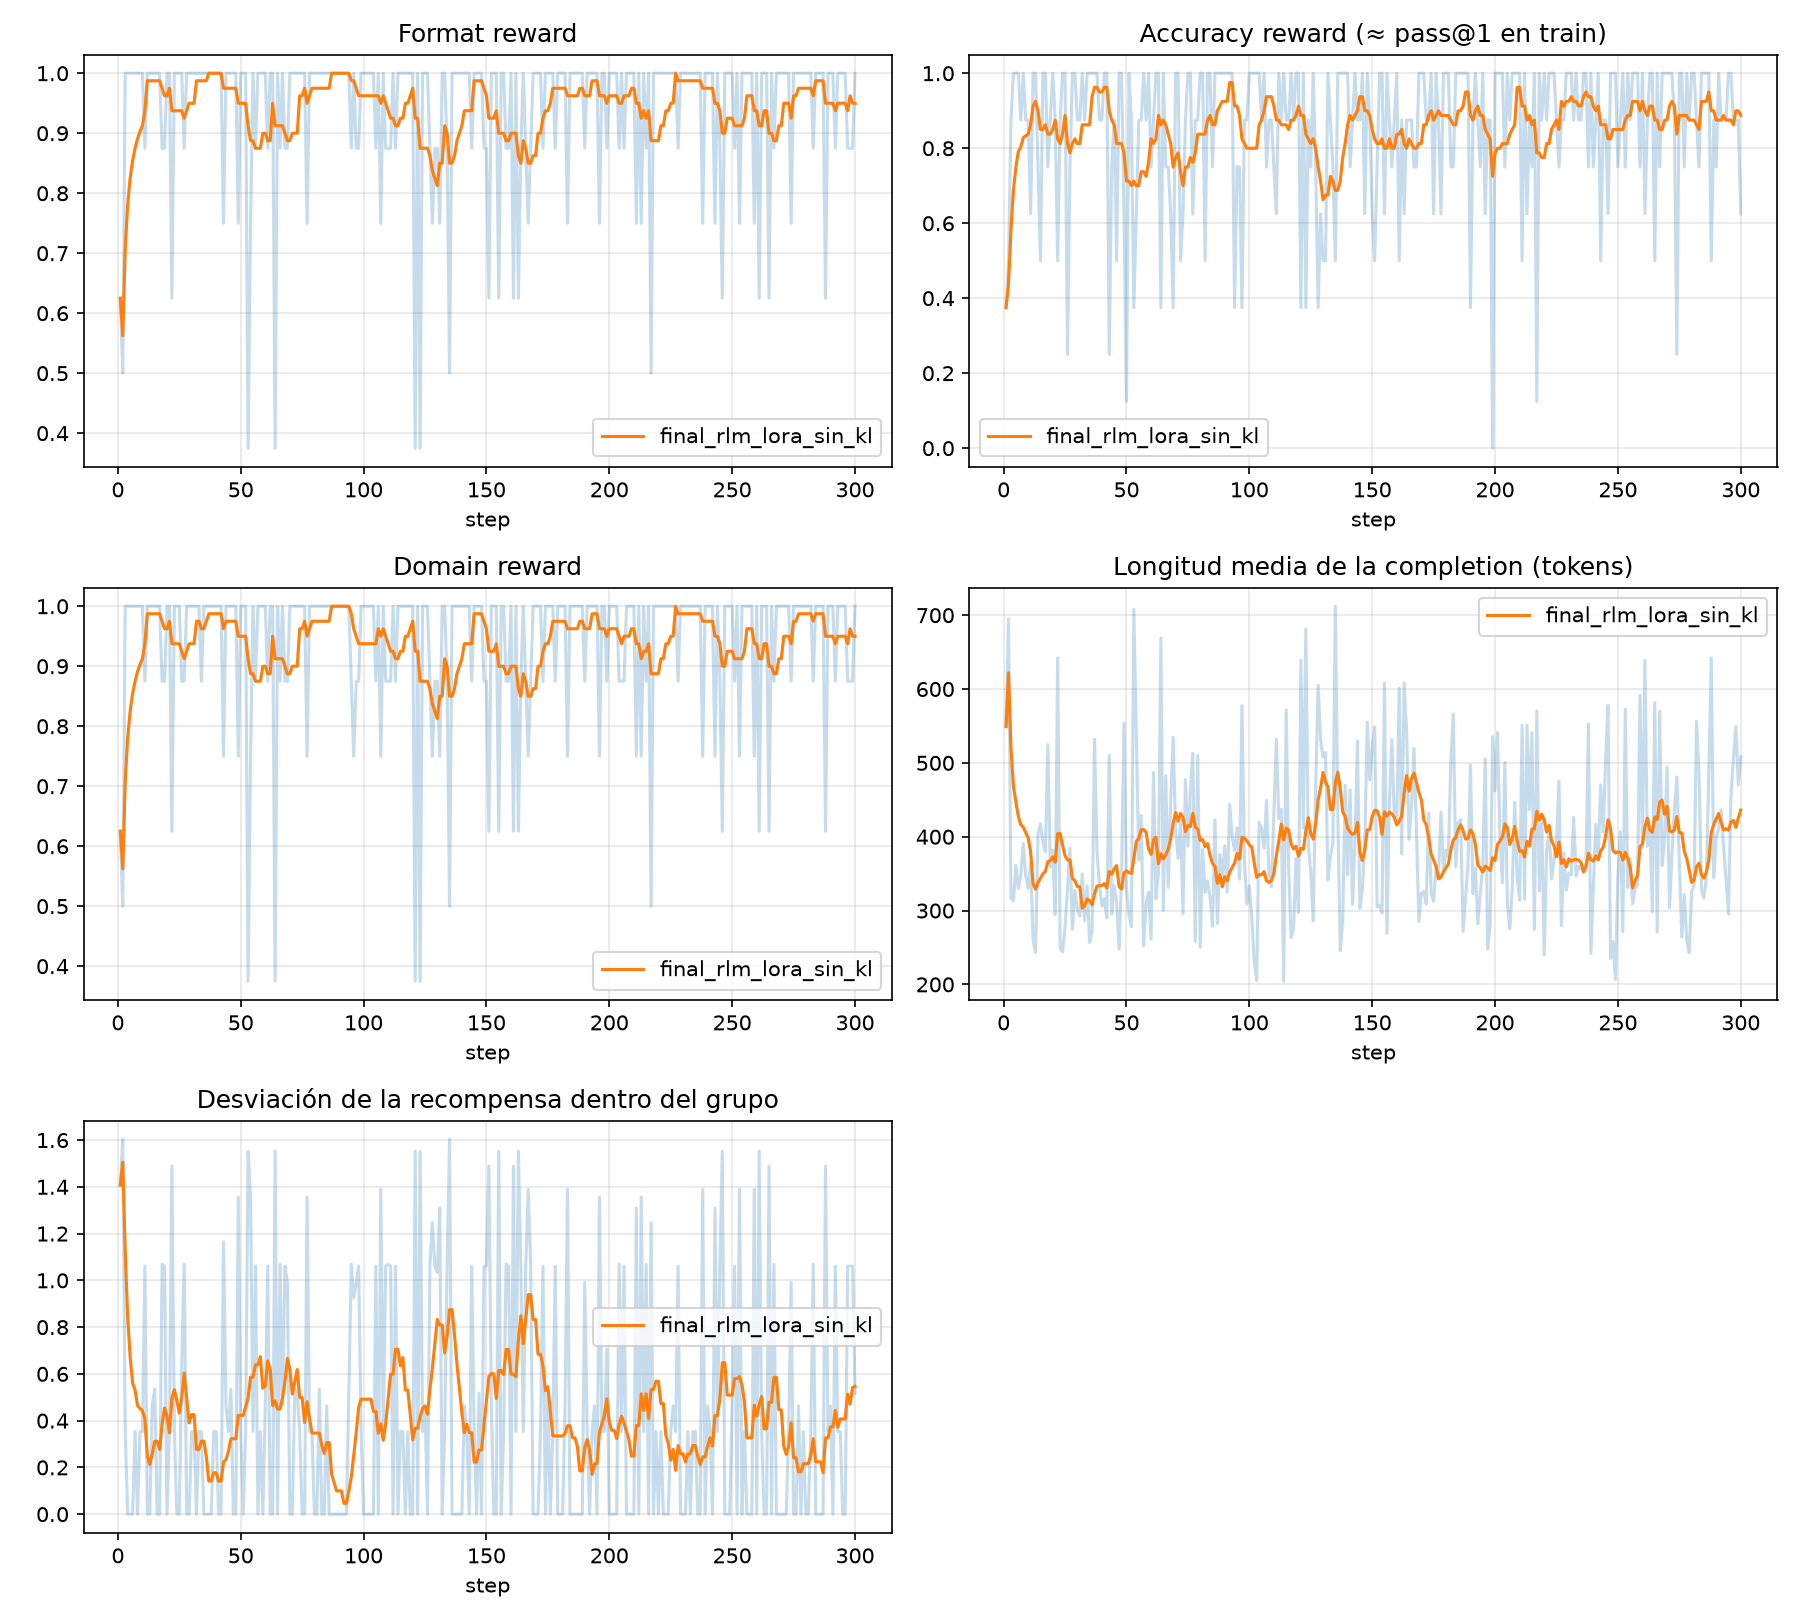
\includegraphics[width=0.85\textwidth]{final_rlm_lora_sin_kl.png}
    \caption{GRPO sin penalización KL y 8 generaciones por problema.}
    \label{fig:grpo8full}
\end{figure}

\begin{figure}[H]
    \centering
    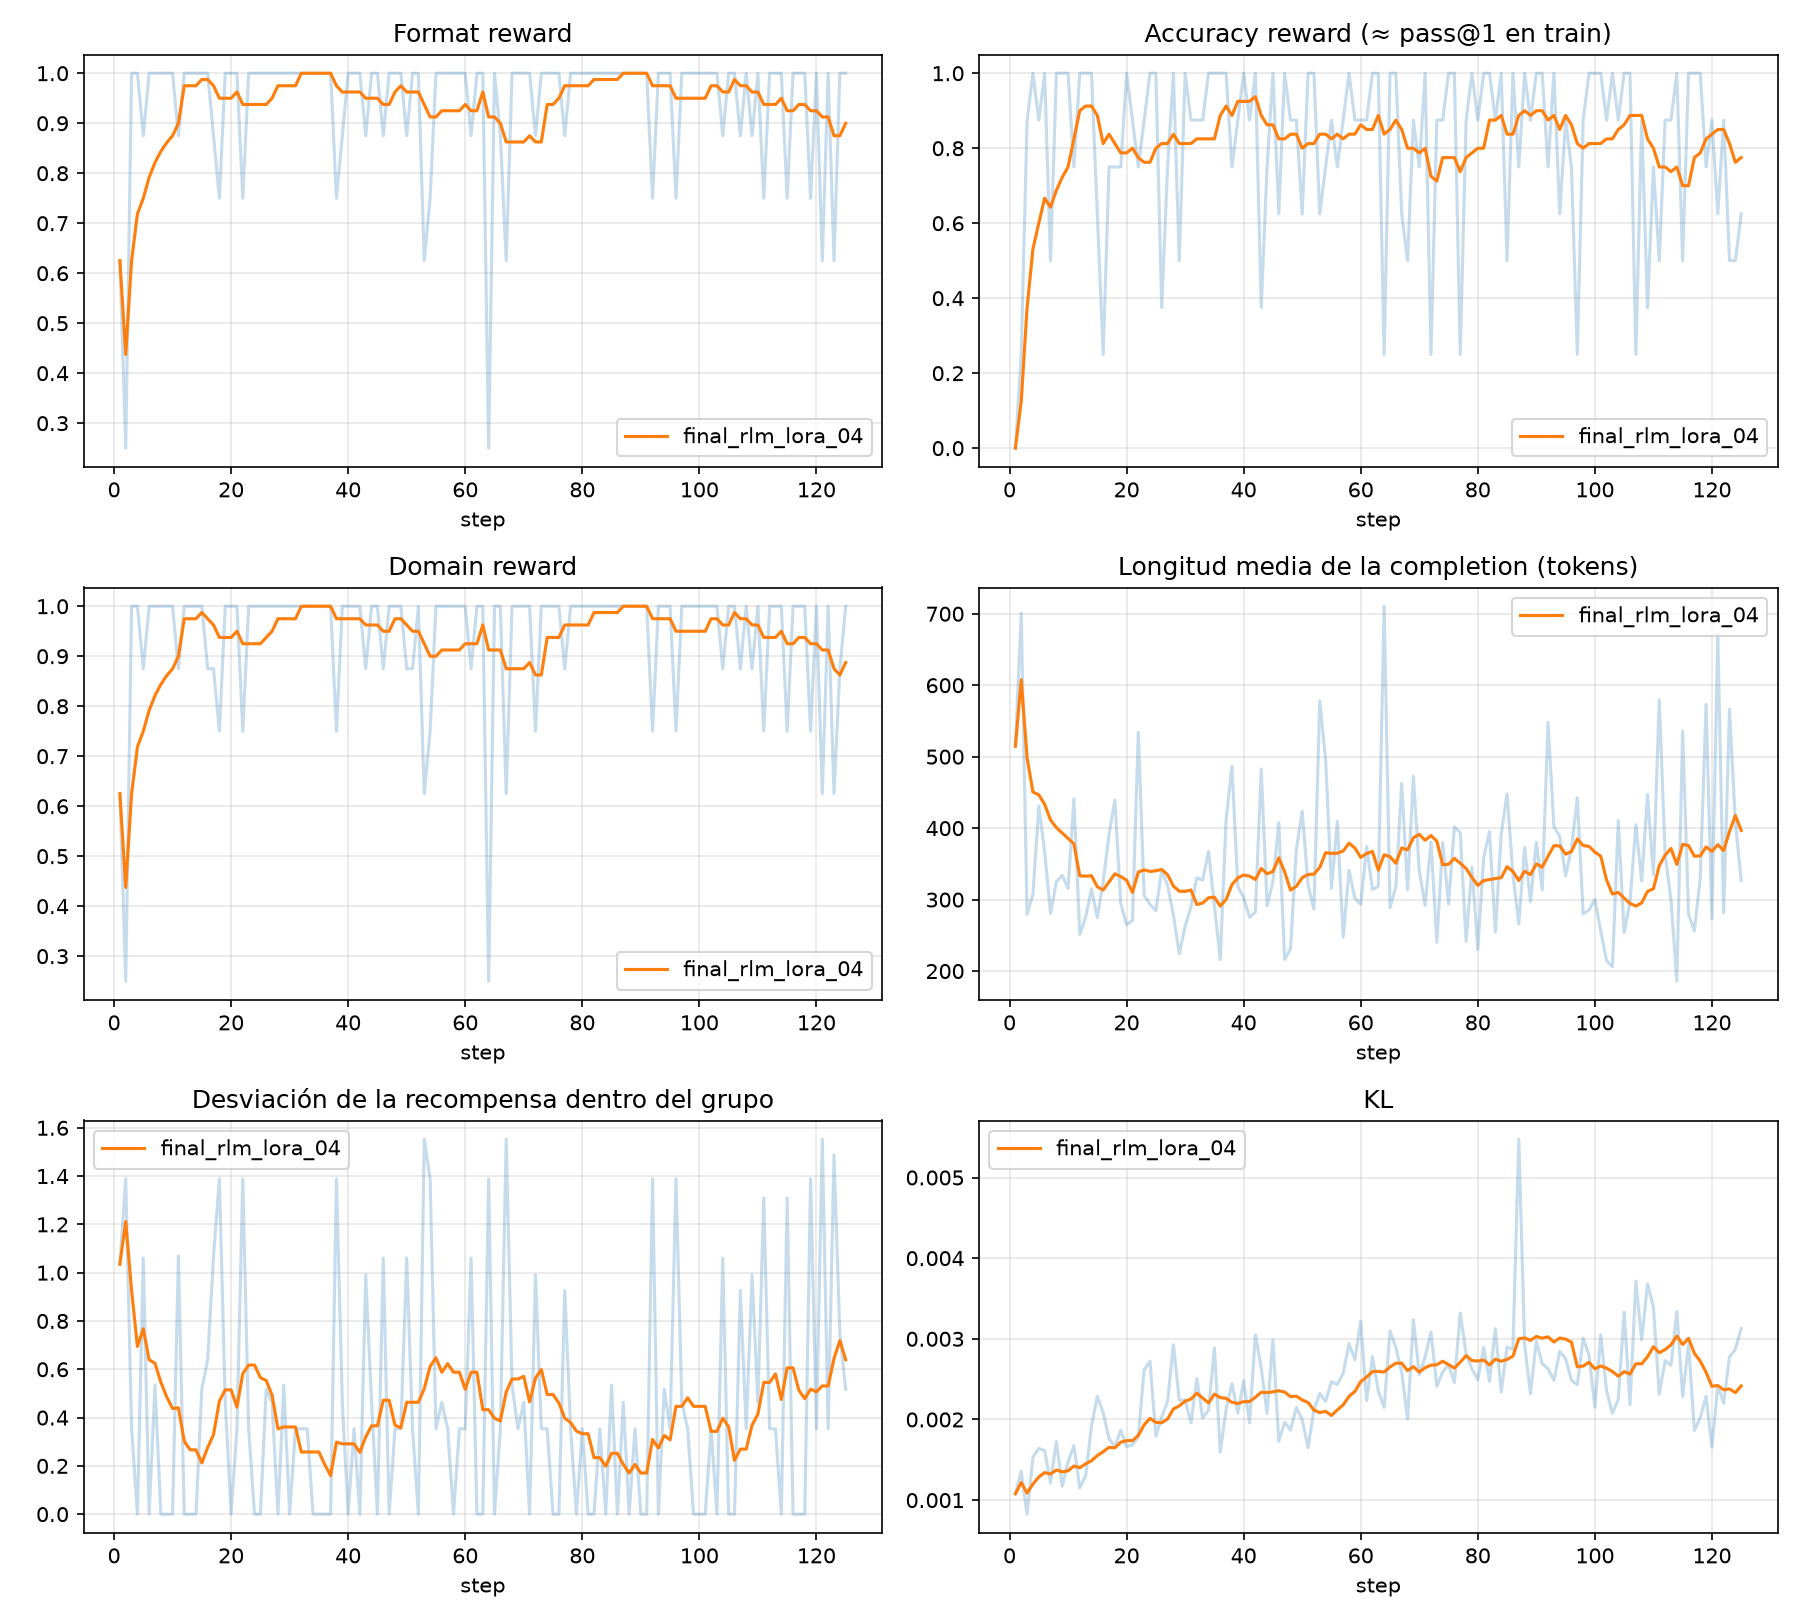
\includegraphics[width=0.85\textwidth]{final_rlm_lora_kl_04.png}
    \caption{GRPO con penalización KL ($\beta = 0{,}04$) y 8 generaciones por problema.}
    \label{fig:grpokl}
\end{figure}

\begin{figure}[H]
    \centering
    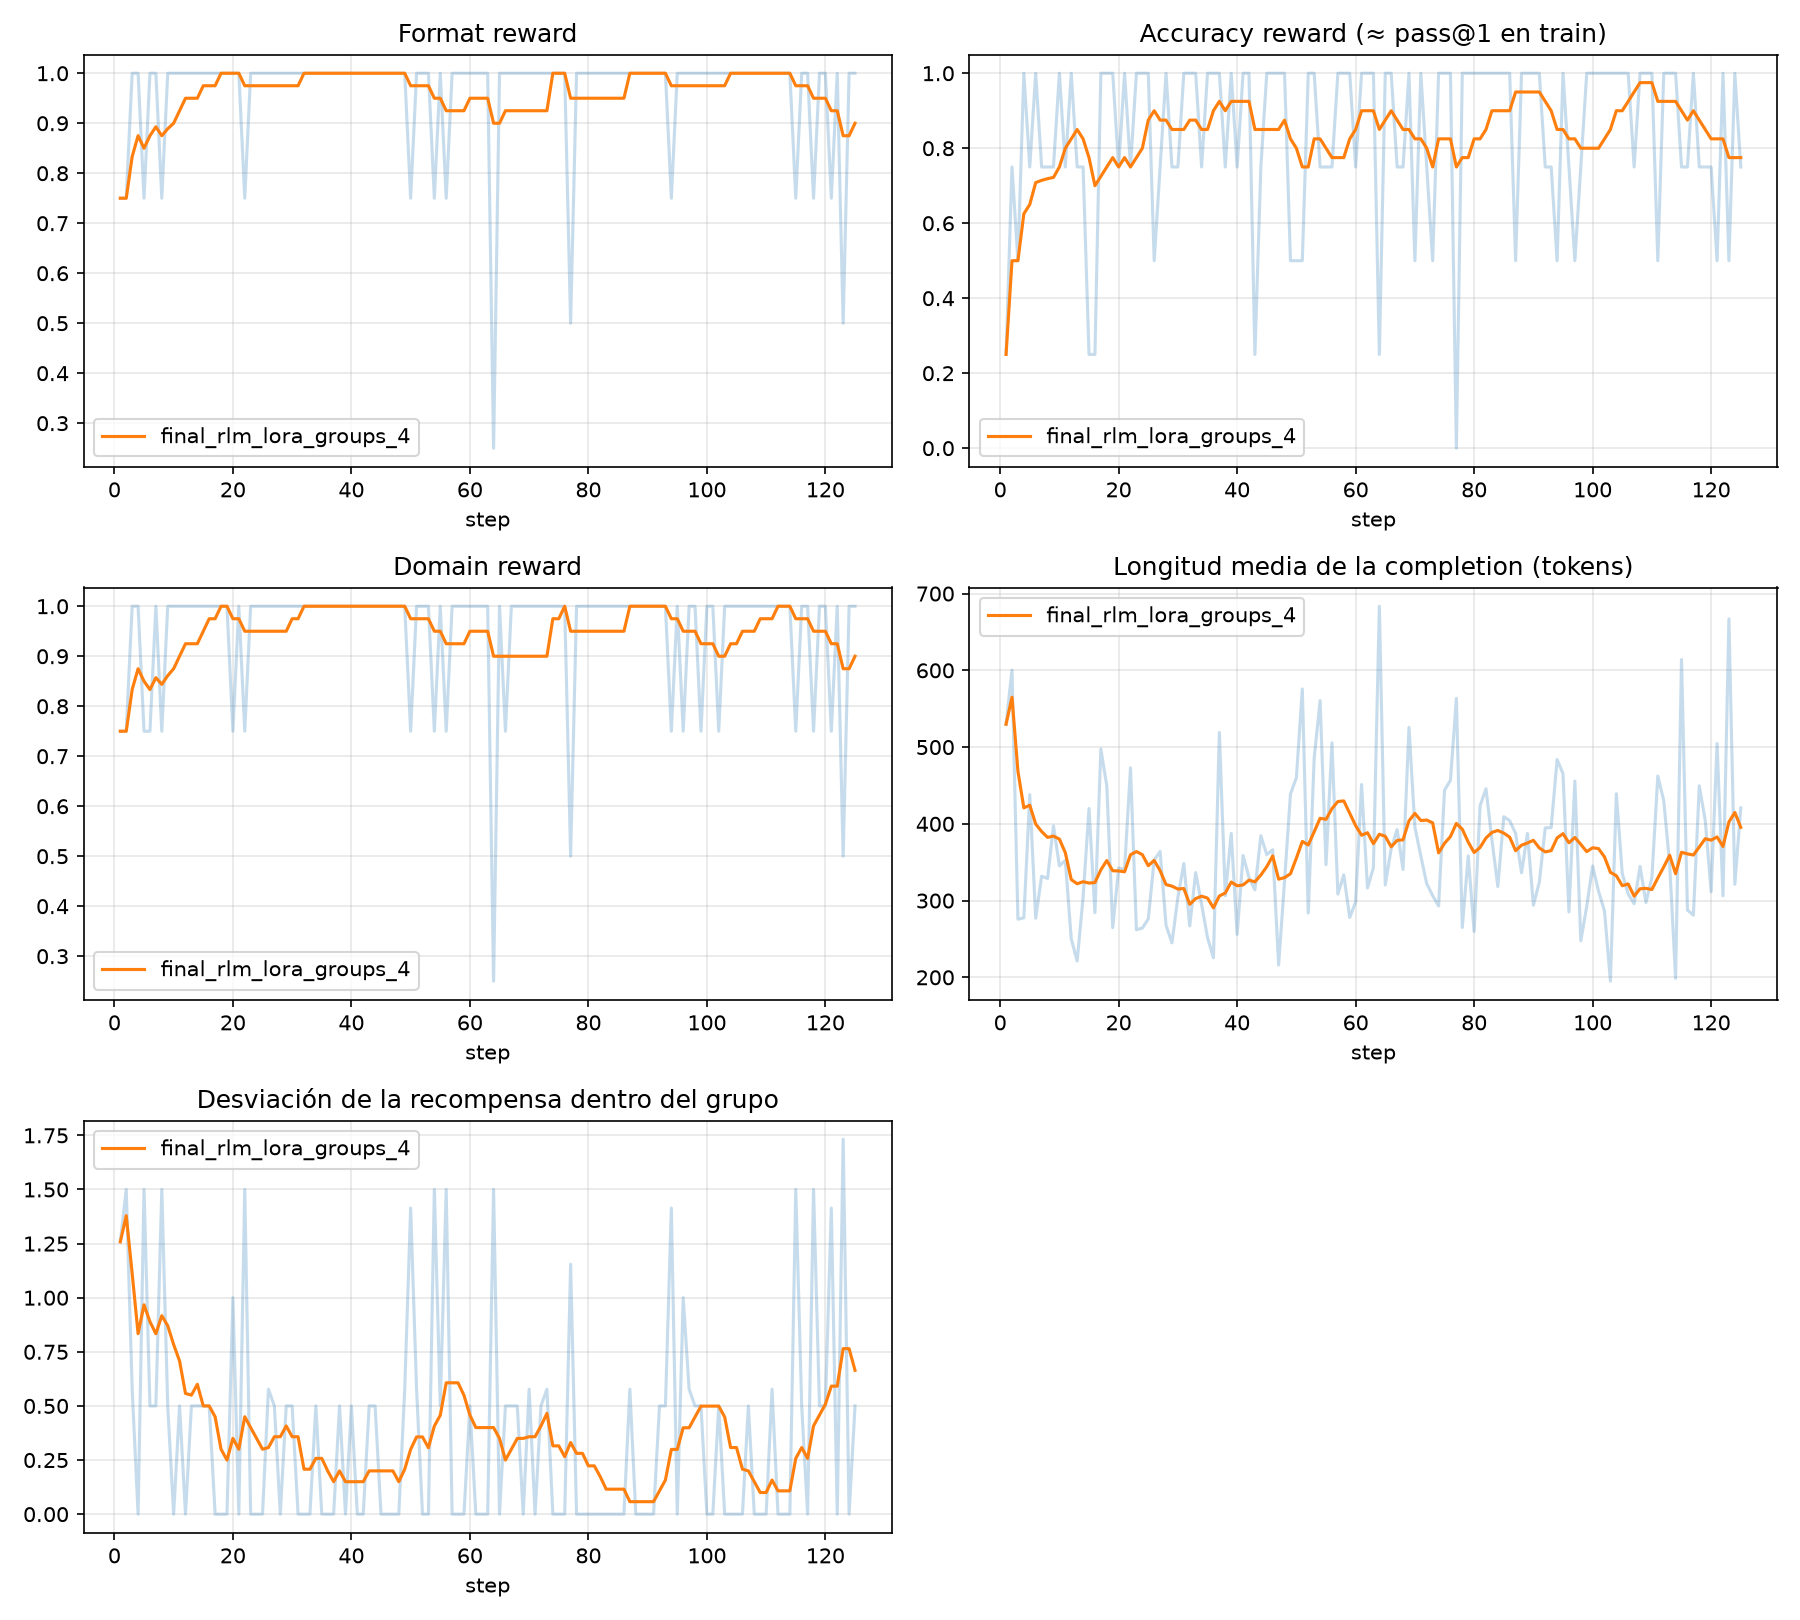
\includegraphics[width=0.85\textwidth]{final_rlm_lora_sin_kl_group_4.png}
    \caption{GRPO sin penalización KL y 4 generaciones por problema.}
    \label{fig:grpo4}
\end{figure}

\section{Conjunto dorado RAG: tipos de pregunta}
\label{anx:gold}
Las 50 preguntas del conjunto dorado de la sección~\ref{sec:fase3} por tipo, con los resultados del híbrido y los fallos de cada tipo.

\begin{table}[H]
    \centering
    \caption{Conjunto dorado por tipo de pregunta con el híbrido ($\lambda = 0{,}4$, chunking recursivo).}
    \label{tab:categorias}
    \small
    \begin{tabular}{lrrr}
        \toprule
        Tipo de pregunta & Preguntas & Recall@5 / MRR & Fallos \\
        \midrule
        Un medicamento, una sección     & 15 & 0,571 / 0,524 & 6 \\
        Un medicamento, varias secciones & 8 & 0,521 / 0,812 & 1 \\
        Varios medicamentos             & 8 & 0,583 / 0,463 & 2 \\
        Inversas (síntoma a fármaco)    & 8 & 1,000 / 1,000 & 0 \\
        Lenguaje coloquial              & 5 & 0,250 / 0,250 & 3 \\
        Premisa dudosa                  & 3 & 0,667 / 0,700 & 1 \\
        Cálculo                         & 3 & 1,000 / 0,567 & 0 \\
        \bottomrule
    \end{tabular}
\end{table}


\section{Repositorio y API}
\begin{itemize}
    \item \textbf{Repositorio:} \url{https://github.com/isamorell/dgm-arca.git}
    \item \textbf{API durante la corrección} (expuesta con \texttt{ngrok http 8000}):\\
    \url{https://family-prodigy-gibberish.ngrok-free.dev}
    \item \textbf{API en local:} \texttt{http://localhost:8000}, con la documentación de los endpoints en \texttt{/docs}.
\end{itemize}

\section{Comandos de reproducción}
Los comandos están sacados de \texttt{EXPERIMENTS.md} (Anexo~\ref{anx:experiments}), donde se explica cada uno. Se ejecutan desde la raíz del repositorio. La API se arranca con \texttt{uv run uvicorn api.app:app --port 8000}.

\subsection*{Fase 1: razonamiento}
\begin{lstlisting}
# Dataset (train, test sin solapamiento con train, y OOD)
uv run python -m rlm.generate_problems --n 800 --split train --out rlm/data/train.jsonl
uv run python -m rlm.generate_problems --n 200 --split test  --out rlm/data/test.jsonl --avoid rlm/data/train.jsonl
uv run python -m rlm.generate_problems --n 100 --split ood   --out rlm/data/test_ood.jsonl

# Destilación y SFT
uv run python -m rlm.distill --data rlm/data/train.jsonl --samples 4 \
  --batch-size 2 --max-new-tokens 1200 \
  --raw-output outputs/distill/raw.jsonl --output rlm/data/sft_traces.jsonl
uv run python -m rlm.train_sft --data rlm/data/sft_traces.jsonl --output rlm/weights/sft_lora

# GRPO: sin KL, con KL (beta 0.04) y con 4 generaciones
uv run python -m rlm.train_grpo --data rlm/data/train.jsonl --init-adapter rlm/weights/sft_lora
uv run python -m rlm.train_grpo --data rlm/data/train.jsonl --init-adapter rlm/weights/sft_lora --beta 0.04
uv run python -m rlm.train_grpo --data rlm/data/train.jsonl --init-adapter rlm/weights/sft_lora --num-generations 4

# Evaluación en test y análisis de los resultados
uv run python -m rlm.evaluate --data rlm/data/test.jsonl --adapters base=none sft=rlm/weights/sft_lora grpo_sin_kl=rlm/weights/final_rlm_lora_sin_kl grpo=rlm/weights/final_rlm_lora_04
uv run python -m rlm.evaluate --data rlm/data/test.jsonl --adapters grpo_group_4=rlm/weights/final_rlm_lora_sin_kl_group_4
uv run python -m rlm.analyze_eval

# Curvas de entrenamiento (ejemplo: 4 generaciones)
uv run python -m rlm.plot_curves rlm/weights/final_rlm_lora --output reports/rlm/final_rlm_lora_sin_kl_group_4/curves_grpo

# Fuera de distribución
uv run python -m rlm.evaluate --data rlm/data/test_ood.jsonl \
  --adapters sft=rlm/weights/sft_lora grpo_sin_kl=rlm/weights/final_rlm_lora_sin_kl \
  --out reports/phase1_eval_ood.json --history reports/phase1_pass1_ood.png
uv run python -m rlm.compare_ood --rescore --models sft grpo_sin_kl
\end{lstlisting}

\subsection*{Fase 2: herramientas}
\begin{lstlisting}
uv run python -m pytest tests/test_tool_registry.py -v

# Banco de herramientas: Qwen3-0.6B y Qwen3-1.7B
uv run python -m tool_use.evaluate --model-id Qwen/Qwen3-0.6B --out reports/phase2_eval_qwen3-0.6b.json
uv run python -m tool_use.evaluate --model-id Qwen/Qwen3-1.7B --out reports/phase2_eval_qwen3-1.7b.json

# Con nuestro modelo (GRPO sin KL y SFT)
uv run python -m tool_use.evaluate --adapter rlm/weights/final_rlm_lora_sin_kl --thinking \
  --no-tools-prompt phase1 --out reports/phase2_eval_qwen3-0.6b_grpo.json
uv run python -m tool_use.evaluate --adapter raquelfes11/dgm-arca-sft-lora --thinking \
  --no-tools-prompt phase1 --out reports/phase2_eval_qwen3-0.6b_sft.json

# Descripciones sin ejemplos
uv run python -m tool_use.evaluate --conditions tools \
  --out reports/phase2_eval_qwen3-0.6b_desc.json
uv run python -m tool_use.evaluate --conditions tools --adapter raquelfes11/dgm-arca-sft-lora \
  --thinking --no-tools-prompt phase1 --out reports/phase2_eval_qwen3-0.6b_sft_desc.json
\end{lstlisting}

\subsection*{Fase 3: conocimiento}
\begin{lstlisting}
# Umbral del chunking semantico
uv run python -m rag.chunking --doc ceftriaxona --sweep 0.15 0.2 0.25 0.3 0.4 0.5 0.6 0.7 0.75 0.8 0.85 --threshold 0.75 --out reports/rag/chunking_distances.png
uv run python -m rag.evaluate --gold rag/gold/gold.jsonl --k 5 --thresholds 0.5 0.6 0.65 0.7 0.75 0.8 0.85 0.9 --out reports/phase3_threshold_sweep.json

# Chunkings, retrievers y barrido de lambda
uv run python -m rag.evaluate --gold rag/gold/gold.jsonl --k 5 --out reports/phase3_eval.json

# Instruccion de la consulta en los embeddings
uv run python -m rag.evaluate --gold rag/gold/gold.jsonl --k 5 --lam 0.4 --instruction-sweep

# Citas de cuatro generadores
ARCA_RLM_BASE_MODEL=Qwen/Qwen3-0.6B uv run python -m rag.compare_generators --tag qwen3-0.6b-base
ARCA_RLM_BASE_MODEL=Qwen/Qwen3-0.6B ARCA_RLM_ADAPTER=rlm/weights/final_rlm_lora_sin_kl \
  uv run python -m rag.compare_generators --tag qwen3-0.6b-rlm
ARCA_RLM_BASE_MODEL=Qwen/Qwen3-1.7B uv run python -m rag.compare_generators --tag qwen3-1.7b
ARCA_RLM_BASE_MODEL=Qwen/Qwen3-4B   uv run python -m rag.compare_generators --tag qwen3-4b
\end{lstlisting}

\subsection*{Fase 4: agente}
\begin{lstlisting}
uv run pytest tests/test_react_agent.py
uv run python -m agent.measure_latency
uv run python -m agent.measure_context_size
uv run python -m agent.validate_bench

# Evaluación de los tres cerebros en el banco de tareas
export ARCA_RLM_ADAPTER=rlm/weights/final_rlm_lora_sin_kl
export ARCA_RLM_ADAPTER_REPO=isamorell/dgm-arca-rlm-lora-sin-kl
uv run python -m agent.evaluate --bench agent/bench/tasks.jsonl --brains base rlm thinking
uv run python -m agent.analyze_eval --markdown reports/phase4_analysis.md
\end{lstlisting}

\section{EXPERIMENTS.md}
\label{anx:experiments}
Copia íntegra del cuaderno de experimentos \texttt{EXPERIMENTS.md} del repositorio.

% Generado a partir de docs/EXPERIMENTS.md (pandoc, sin cambios en el contenido).
\begingroup\raggedright\sloppy
Copiad esta plantilla a la raíz de vuestro repositorio como \texttt{EXPERIMENTS.md} y añadid una
entrada cada vez que lancéis algo o toméis una decisión. Con fecha. No lo escribáis al final
de memoria: dentro de un mes no recordaréis por qué bajasteis la tasa de aprendizaje.

Una entrada honesta que diga "probamos X, no funcionó, creemos que por Y" vale más que diez
que digan "todo bien". Esto es lo primero que leo cuando corrijo interpretación.

\begin{center}\rule{0.5\linewidth}{0.5pt}\end{center}

\subsection{Formato de cada entrada}

\begin{lstlisting}
### AAAA-MM-DD · Fase N · Título corto

**Qué queríamos saber.** La pregunta o la hipótesis.
**Qué hicimos.** Comando exacto, modelo, datos, hiperparámetros que cambian respecto a la
entrada anterior.
**Qué pasó.** Números, curva (enlace a reports/), ejemplos.
**Qué concluimos.** Y qué hacemos a continuación.
\end{lstlisting}

\begin{center}\rule{0.5\linewidth}{0.5pt}\end{center}

\subsection{Ejemplo}

\subsubsection{2026-10-02 · Fase 1 · Primer GRPO sobre nuestro dataset}

\textbf{Qué queríamos saber.} Si el modelo aprende el formato con nuestro prompt de sistema antes
de preocuparnos por la exactitud.

\textbf{Qué hicimos.} \texttt{uv run python -m rlm.train\_\allowbreak{}grpo -\/\allowbreak{}-data rlm/\allowbreak{}data/\allowbreak{}train.jsonl -\/\allowbreak{}-steps 100 -\/\allowbreak{}-num-generations 8 -\/\allowbreak{}-max-completion-length 512} partiendo del adaptador de SFT. Sin KL.

\textbf{Qué pasó.} La recompensa de formato pasa de 0.31 a 0.97 en 40 pasos. La de exactitud sube
de 0.18 a 0.26 y se estanca. La longitud media baja de 480 a 210 tokens: el modelo aprende a
cerrar la etiqueta antes de quedarse sin presupuesto. Curva en \texttt{reports/\allowbreak{}grpo\_\allowbreak{}run01.png}.

\textbf{Qué concluimos.} El formato está resuelto. La exactitud se estanca porque el 40 \% de los
problemas del dataset tienen respuestas con unidades y el verificador numérico las ignora:
"120 litros" y "120" cuentan igual, pero "0.12 m³" cuenta como fallo. Siguiente paso:
normalizar unidades en el verificador y repetir.

\begin{center}\rule{0.5\linewidth}{0.5pt}\end{center}

\subsection{Entradas}

\subsubsection{2026-09-28 · Fase 1 · Generación de problemas}

\textbf{Qué queríamos saber.} Si los valores de dosis, concentraciones y volúmenes del generador
tenían que salir de datos reales (p.ej. fichas técnicas de CIMA) o bastaba con rangos inventados.

\textbf{Qué hicimos.} Valoramos extraer posologías y presentaciones reales de CIMA. Lo descartamos
para la fase 1: los datos de posología y dilución están en texto libre, dependen de la indicación,
la edad y la vía, y extraerlos exigiría que alguien del equipo leyese cada ficha y sacase los
números a mano. En su lugar, muestreamos de listas de valores redondos (p.ej. dosis 5, 10, 25 mg;
viales 100mg/5mL) y descartamos los problemas cuya respuesta cae fuera de un rango plausible
(\texttt{BOUNDS} en \texttt{generate\_\allowbreak{}problems.py}).

El generador utiliza la plantilla de \texttt{generate\_\allowbreak{}problems.py} (estrategia 1 de \texttt{datasets.md}):
un sorteo de parámetros, una implementación de referencia (\texttt{solve}) que es a la vez el verificador,
y varias plantillas de enunciado. Toda la aritmética se hace con \texttt{Fraction}, de modo que el resultado
es exacto y el redondeo es siempre half-up. Se usa \texttt{Fraction} en lugar de Pint porque es exacto
y determinista; Pint se usará en la herramienta de cálculo de la fase 2, como decía la propuesta.

Comandos (semilla por defecto, \texttt{DEFAULT\_\allowbreak{}SEED =\allowbreak{} 0}):

\begin{lstlisting}
uv run python -m rlm.generate_problems --n 800 --split train --out rlm/data/train.jsonl
uv run python -m rlm.generate_problems --n 200 --split test  --out rlm/data/test.jsonl --avoid rlm/data/train.jsonl
uv run python -m rlm.generate_problems --n 100 --split ood   --out rlm/data/test_ood.jsonl
\end{lstlisting}

\textbf{Qué pasó.} El generador produce problemas con la aritmética correcta, pero las dosis no son
clínicamente realistas en todos los casos. Ejemplos de \texttt{train.jsonl}: metronidazol a
100 mg/kg/día y a 1000 mcg/kg/día, y ceftriaxona a 500 mcg/kg/día. La dosis habitual de cada
fármaco es muy distinta de esos valores. Un 10 \% de los enunciados (78 de 800) no lleva nombre
de fármaco.

\textbf{Qué concluimos.} Para la fase 1 el objetivo es evaluar si el modelo razona con unidades y
conversiones, y eso no depende de que el fármaco sea real: la respuesta se verifica contra el
cálculo, no contra un manual de farmacología. Es una limitación asumida y la dejamos escrita en el
informe: el modelo entrenado sabe calcular, no sabe qué dosis es adecuada. Las concentraciones y
presentaciones reales entran en la fase 2 (CIMA) y la fase 3 (RAG).

\begin{center}\rule{0.5\linewidth}{0.5pt}\end{center}

\subsubsection{2026-09-28 · Fase 1 · Diseño de las plantillas de los enunciados}

\textbf{Qué queríamos saber.} Cómo conseguir enunciados lo bastante variados para que el modelo
aprenda la tarea y no la plantilla.

\textbf{Qué hicimos.} La idea inicial era usar unas 7 plantillas de enunciado y rellenarlas con
parámetros aleatorios. La descartamos porque el modelo vería solo esas 7 estructuras con los
números cambiados. En su lugar:

\begin{itemize}
\tightlist
\item
  separamos 7 familias de problema (velocidad de bomba, goteo, dosis por peso y día, volumen a
  administrar, infusión mcg/kg/min, su inversa y diluciones), cada una con 3-4 plantillas
  completas (26 en total);
\item
  variamos la pregunta final (3-5 formulaciones por familia) y la petición de redondeo;
\item
  añadimos cuatro estilos de escritura compuestos a partir de datos sueltos: narrativo,
  telegráfico, lista y línea de datos, con el orden de los datos aleatorio;
\item
  variamos la coma o el punto decimal, las unidades (mL/ml, mcg/µg), la forma de escribir el
  tiempo (4 h, 240 min, 1 h 30 min) y añadimos datos irrelevantes (cama, hora, vía) en un 35 \%
  de los problemas.
\end{itemize}

\textbf{Qué pasó.} Contamos esqueletos distintos, es decir, enunciados con los números
enmascarados: 763 de 800 en train (95 \%), 193 de 200 en test y 96 de 100 en OOD. Reparto de
estilos en train: cohesivo 244, narrativo 248, telegráfico 133, lista 84, datos 91. Con 7
plantillas fijas el máximo habría sido del orden de 7 esqueletos.

\textbf{Qué concluimos.} La variedad de redacción es alta. Es variedad léxica y de estructura: las
familias siguen siendo 7, así que el modelo no ve tipos de problema nuevos, solo formas nuevas
de escribirlos.

\begin{center}\rule{0.5\linewidth}{0.5pt}\end{center}

\subsubsection{2026-09-30 · Fase 1 · Desequilibrio entre familias en los datasets}

\textbf{Qué queríamos saber.} Si los datasets quedaban equilibrados entre familias y niveles de
dificultad, y si test tiene la misma distribución que train.

\textbf{Qué hicimos.} Contamos problemas por familia y por nivel (campo \texttt{branches}) en train, test y
OOD de la primera versión del generador.

\textbf{Qué pasó.} Con sorteos equilibrados saldrían unos 160 problemas por familia en train. No fue
así:

{\def\LTcaptype{none} % do not increment counter
\footnotesize\setlength{\tabcolsep}{3pt}
\begin{longtable}[]{@{}llllll@{}}
\toprule\noalign{}
Primera versión & pump & drops & dose\_\allowbreak{}day & volume & dilution \\
\midrule\noalign{}
\endhead
\bottomrule\noalign{}
\endlastfoot
train (800) & 82 & 156 & 239 & 220 & 103 \\
test (200) & 12 & 34 & 74 & 69 & 11 \\
\end{longtable}
}

El nivel 3 (dosis por peso y volumen) era el 57 \% de train y el 72 \% de test, y el nivel 1 solo
el 14 \% de train y el 6 \% de test. La causa: \texttt{pump} y \texttt{dilution} tenían un espacio de
parámetros pequeño (en \texttt{pump}, el volumen salía de 5 valores fijos 5 de cada 6 veces, así que
solo había 29 volúmenes distintos y 82 problemas únicos). La deduplicación descartaba los
repetidos y las demás familias ocupaban ese sitio. Además, test se genera con \texttt{-\/\allowbreak{}-avoid} sobre
train y solo recibía las combinaciones que train había dejado libres. Con 12 y 11 problemas de
\texttt{pump} y \texttt{dilution} en test no se podía analizar el pass@1 por familia.

\textbf{Qué hicimos.} Dos cambios en \texttt{generate\_\allowbreak{}problems.py}:

\begin{enumerate}
\tightlist
\item
  Espacios de parámetros más grandes: el tiempo pasa de 13 valores a uno cada 15 minutos
  entre 30 min y 12 h (más 24 h); el volumen es una bolsa estándar el 40 \% de las veces y en
  el resto cualquier múltiplo de 10 mL; las diluciones tienen más dosis, más concentraciones
  objetivo y más volúmenes de reconstitución.
\item
  Cuotas por familia en \texttt{generate}: cada familia recibe el mismo número de problemas en vez de
  sortear la familia al azar, y el resultado se mezcla al final. Si una familia no puede
  producir su cuota de problemas únicos, el script falla con un mensaje que la nombra.
\end{enumerate}

Regeneramos los tres ficheros con los mismos comandos y la misma semilla.

\textbf{Qué pasó (después).}

{\def\LTcaptype{none} % do not increment counter
\footnotesize\setlength{\tabcolsep}{3pt}
\begin{longtable}[]{@{}llllll@{}}
\toprule\noalign{}
Segunda versión & pump & drops & dose\_\allowbreak{}day & volume & dilution \\
\midrule\noalign{}
\endhead
\bottomrule\noalign{}
\endlastfoot
train (800) & 160 & 160 & 160 & 160 & 160 \\
test (200) & 40 & 40 & 40 & 40 & 40 \\
\end{longtable}
}

OOD: 50 \texttt{infusion} y 50 \texttt{infusion\_\allowbreak{}inverse}. Niveles 1 / 2 / 3 en train: 231 / 249 / 320 (29 \%,
31 \%, 40 \%); en test: 50 / 70 / 80 (25 \%, 35 \%, 40 \%). El solapamiento entre ficheros sigue en
0. Capacidad: train llega sin problema a 3.000 problemas y el límite (unos 3.200) lo marcan las
diluciones, con 653 combinaciones únicas.

Queda un desequilibrio menor dentro de \texttt{dilution}: en train hay 89 problemas de diluyente y 71
de volumen final, y en test 30 de diluyente y 10 de volumen final. Los problemas de volumen
final tienen menos combinaciones y train ya se ha llevado buena parte de ellas, así que
\texttt{-\/\allowbreak{}-avoid} deja pocas para test.

\textbf{Qué concluimos.} Las familias ya están equilibradas y se puede analizar el pass@1 por
familia con 40 problemas cada una en test. Con solo 10 problemas de volumen final en test, el
resultado de ese subtipo de dilución no es fiable, y lo trataremos con cautela en el análisis.

\begin{center}\rule{0.5\linewidth}{0.5pt}\end{center}

\subsubsection{2026-10-04 · Fase 1 · Definición de la recompensa de dominio}

\textbf{Qué queríamos saber.} Queríamos definir una recompensa de dominio que fuese importante para nuestra tarea de ayudar a estudiantes de enfermería

\textbf{Qué hicimos.} Decidimos que lo mejor era tener una recompensa que penalizase al modelo no utilizar las unidades que pedía el modelo. Para permitirle un poco más de flexibilidad, tenemos en cuenta que las mismas unidades pueden escribirse de distintas formas. Por ejemplo, gotas por minuto se puede abreviar en gotas/min.

También incluimos estas diferentes formas en la extracción de la unidad, que se realiza con cuidado para extraer la unidad que acompaña a la respuesta final y no otra unidad que puede que acompañe a un número distinto.

\textbf{Qué pasó.} Generamos diferentes aliases para cada unidad con el fin de poder comparar las diferentes formas en las que referenciamos una misma unidad. Estos los incluimos también en el patrón de regex para extraer las unidades de las respuestas

\textbf{Qué concluimos.} Así podremos evaluar la correcta extracción de unidades como la recompensa de dominio.

\begin{center}\rule{0.5\linewidth}{0.5pt}\end{center}

\subsubsection{2026-10-07 · Fase 1 · Destilación: trazas de razonamiento con Qwen3-4B}

\textbf{Qué queríamos saber.} Cuántas trazas verificadas conseguimos con un teacher de 4B en modo
thinking sobre nuestros 800 problemas de train, si razona en español, y qué familias o niveles
le cuestan más (primera medida de lo difícil que es el dominio).

\textbf{Qué hicimos.} Teacher \texttt{Qwen/\allowbreak{}Qwen3-4B} en modo thinking, muestreo con los valores de su ficha
(temperatura 0.6, top-p 0.95, top-k 20, nunca greedy), 4 trazas por problema sobre
\texttt{rlm/\allowbreak{}data/\allowbreak{}train.jsonl}, límite de 1200 tokens nuevos. Cada traza se pasa por un único juez
(\texttt{rlm/\allowbreak{}distill.py}): se reescribe a \texttt{\textless{}think\textgreater{}…\textless{}/\allowbreak{}think\textgreater{}\textless{}answer\textgreater{}…\textless{}/\allowbreak{}answer\textgreater{}}, se verifica con
\texttt{MedicationVerifier} (valor \textbf{y} unidad) y se descarta con un motivo único. Para el SFT se
guardan como máximo las 2 trazas verificadas más cortas de cada problema.

\begin{lstlisting}
uv run python -m rlm.distill --data rlm/data/train.jsonl --samples 4 \
  --batch-size 2 --max-new-tokens 1200 \
  --raw-output outputs/distill/raw.jsonl --output rlm/data/sft_traces.jsonl
\end{lstlisting}

Antes de la ejecución completa hubo tres decisiones tomadas con pruebas pequeñas:

\begin{enumerate}
\tightlist
\item
  \textbf{Idioma.} En una primera prueba (20 generaciones, 512 tokens) las 2 trazas que terminaron
  eran correctas pero razonaban en inglés, aunque el enunciado y la instrucción estaban en
  español. Pedirle español en el prompt no bastó, así que se arranca su razonamiento en español
  (el prompt acaba con \texttt{\textless{}think\textgreater{}} y la frase "Vale, voy a resolverlo paso a paso."). Esa frase
  queda como inicio de cada traza. Se descartan las trazas que no son mayoritariamente españolas.
\item
  \textbf{Piloto} (40 problemas, 160 generaciones, \textasciitilde30 min): 147 verificadas (91,9 \%). La longitud
  de las generaciones tenía mediana 474 tokens, percentil 95 en 954 y solo el 1 \% llegaba al
  límite de 2048. Por eso se bajó el límite a 1200 en la ejecución completa: acorta los lotes
  lentos y pierde pocas trazas.
\item
  \textbf{Dos fallos del juez, vistos en el piloto.} Una respuesta correcta escrita en LaTeX
  (\texttt{20\{,\}20 mL}) se contaba como mal porque el verificador leía dos números; ahora se limpia
  antes de verificar. Y el prefill acababa en un espacio que el teacher imitaba, dejando dobles
  espacios tras cada punto; se quitó el espacio y se normalizan los espacios al construir la traza.
  De los 8 \texttt{wrong\_\allowbreak{}value} del piloto, 7 eran errores de aritmética reales del teacher (por
  ejemplo 740 mL en 315 min es 140,95 → 141,0, y contestó 141,1 las tres veces): la respuesta de
  referencia del generador era la correcta.
\end{enumerate}

\textbf{Qué pasó.} 3200 generaciones (800 problemas × 4):

\begin{itemize}
\tightlist
\item
  Verificadas: \textbf{3005 (93,9 \%)}. Problemas con al menos una traza verificada: \textbf{788/800}.
  Longitud media de las trazas aceptadas: 570 tokens. Pasan al SFT \textbf{1557 trazas} (máximo 2 por
  problema).
\item
  Motivos de rechazo (195 generaciones): \texttt{truncated} 164, \texttt{wrong\_\allowbreak{}value} 25, \texttt{wrong\_\allowbreak{}unit} 6;
  \texttt{no\_\allowbreak{}answer}, \texttt{bad\_\allowbreak{}format}, \texttt{too\_\allowbreak{}short}, \texttt{not\_\allowbreak{}spanish} y \texttt{too\_\allowbreak{}long} 0.
\end{itemize}

{\def\LTcaptype{none} % do not increment counter
\small\setlength{\tabcolsep}{3pt}
\begin{longtable}[]{@{}llll@{}}
\toprule\noalign{}
Familia & Generadas & Verificadas & Tasa \\
\midrule\noalign{}
\endhead
\bottomrule\noalign{}
\endlastfoot
dilution & 640 & 501 & 78,3 \% \\
dose\_\allowbreak{}day & 640 & 629 & 98,3 \% \\
drops & 640 & 625 & 97,7 \% \\
pump & 640 & 621 & 97,0 \% \\
volume & 640 & 629 & 98,3 \% \\
\end{longtable}
}

{\def\LTcaptype{none} % do not increment counter
\small\setlength{\tabcolsep}{3pt}
\begin{longtable}[]{@{}llll@{}}
\toprule\noalign{}
Nivel & Generadas & Verificadas & Tasa \\
\midrule\noalign{}
\endhead
\bottomrule\noalign{}
\endlastfoot
1 & 924 & 902 & 97,6 \% \\
2 & 996 & 845 & 84,8 \% \\
3 & 1280 & 1258 & 98,3 \% \\
\end{longtable}
}

Duración de la ejecución completa en el DGX (una partición MIG de 16 GiB): unas 6 h (de 09:11 a 15:10 del 7 de octubre), en una sola ejecución sin reanudar..

\textbf{Qué concluimos.}

\begin{itemize}
\tightlist
\item
  El dominio es fácil para el teacher: casi todo lo que se rechaza (164 de 195, el 84 \%) es
  porque no termina de razonar en 1200 tokens, no porque se equivoque (31 respuestas mal de
  3200, el 1 \%). Y las truncadas están casi todas en una familia: \texttt{dilution} acumula 137 de las
  164 (el 21 \% de sus 640 generaciones) y solo 2 respuestas mal; en las otras cuatro familias
  hay entre 3 y 10 truncadas cada una. Es decir, en diluciones (reconstituir, calcular el
  diluyente o el volumen final) el teacher se alarga mucho, pero cuando termina acierta. Por
  niveles, el 2 (84,8 \%) es el más bajo porque es donde caen esas diluciones.
\item
  Los errores reales del teacher están sobre todo en \texttt{pump} (11 de 25 con \texttt{wrong\_\allowbreak{}value}) y
  \texttt{dose\_\allowbreak{}day} (5 de las 6 con \texttt{wrong\_\allowbreak{}unit}).
\item
  Reparto de las 1557 trazas del SFT por familia: dose\_\allowbreak{}day 320, volume 320, drops 319, pump 318,
  dilution 280. El desequilibrio es pequeño (280 frente a \textasciitilde320), pero \texttt{dilution} es también la
  familia con más problemas sin traza verificada (12 problemas en total no tienen ninguna). Si
  el modelo de SFT falla sobre todo en \texttt{dilution} en el test, la primera opción es regenerar solo
  esos problemas con un límite mayor de tokens.
\item
  Las 6 respuestas con el valor correcto y la unidad equivocada (\texttt{wrong\_\allowbreak{}unit}) las habría dado
  por buenas un verificador solo numérico: justifican comprobar la unidad.
\item
  Limitaciones: el juez comprueba la respuesta final, no el razonamiento, así que puede haber
  trazas con respuesta correcta y explicación pobre (hemos visto alguna que describe los pasos
  sin escribir los números intermedios). Tampoco está medido cuánto acorta las trazas el prefill:
  sin él, 18 de 20 generaciones no habían terminado en 512 tokens, y con él la mediana del piloto
  es 474, pero son pruebas con problemas y límites distintos y no se pueden comparar sin más.
\item
  Siguiente paso: SFT con LoRA sobre \texttt{rlm/\allowbreak{}data/\allowbreak{}sft\_\allowbreak{}traces.jsonl} (\texttt{feat\_\allowbreak{}sft}).
\end{itemize}

\begin{center}\rule{0.5\linewidth}{0.5pt}\end{center}

\subsubsection{2026-10-07 · Fase 1 · SFT con LoRA sobre las trazas destiladas}

\textbf{Qué queríamos saber.} Si con las 1557 trazas verificadas un adaptador LoRA sobre
Qwen3-0.6B aprende el formato \texttt{\textless{}think\textgreater{}…\textless{}/\allowbreak{}think\textgreater{}\textless{}answer\textgreater{}…\textless{}/\allowbreak{}answer\textgreater{}} y el estilo de razonamiento
en español, y cuántas épocas conviene.

\textbf{Qué hicimos.} Una sola ejecución, con valores de partida estándar y sin barrido:

\begin{lstlisting}
uv run python -m rlm.train_sft --data rlm/data/sft_traces.jsonl --output rlm/weights/sft_lora
\end{lstlisting}

\begin{itemize}
\tightlist
\item
  Modelo base \texttt{Qwen/\allowbreak{}Qwen3-0.6B}: es el que entrenará GRPO después y cabe con holgura en la
  partición MIG de 16 GiB (el profesor, de la misma familia, ya usa su plantilla de chat).
\item
  LoRA r=16, alpha 32, dropout 0.05, sobre todas las capas lineales. Un arranque en frío enseña
  un formato y un estilo, no conocimiento nuevo, así que un adaptador pequeño basta.
\item
  Learning rate 2e-4 con decaimiento coseno y 5 \% de calentamiento (rango habitual de LoRA:
  1e-4 a 3e-4). 3 épocas. Batch efectivo de 16 (2 × 8 pasos de acumulación). bf16 y
  gradient checkpointing. La pérdida se calcula solo sobre la respuesta del asistente.
\item
  Datos: el 5 \% de los problemas, elegidos por problema y no por traza (cada problema tiene
  dos trazas y así no hay fugas), se reserva para evaluación: 1479 ejemplos de entrenamiento y
  78 de evaluación. Longitudes en tokens (prompt + traza) en train: mediana 476, percentil 95 en
  752, máximo 1177. \texttt{max\_\allowbreak{}length} = 1536, así que no se descartó ni cortó ningún ejemplo.
\item
  Al final de cada época se calcula la pérdida de evaluación y se guarda el adaptador de la
  mejor época.
\end{itemize}

\textbf{Qué pasó.} 279 pasos en 27 minutos. La pérdida de entrenamiento baja de 0,81 en los primeros
pasos a \textasciitilde0,32 al acabar la primera época y a \textasciitilde0,205 al final (media de la ejecución: 0,286).

{\def\LTcaptype{none} % do not increment counter
\small\setlength{\tabcolsep}{3pt}
\begin{longtable}[]{@{}lll@{}}
\toprule\noalign{}
Época & eval\_\allowbreak{}loss & Precisión de token (eval) \\
\midrule\noalign{}
\endhead
\bottomrule\noalign{}
\endlastfoot
1 & 0,2643 & 0,9111 \\
2 & 0,2379 & 0,9164 \\
3 & 0,2337 & 0,9198 \\
\end{longtable}
}

La mejor época por pérdida de evaluación es la 3, que es la que se guarda. Historial completo en
\texttt{rlm/\allowbreak{}weights/\allowbreak{}sft\_\allowbreak{}lora/\allowbreak{}log\_\allowbreak{}history.json}.

Adaptador publicado en Hugging Face: \texttt{raquelfes11/\allowbreak{}dgm-arca-sft-lora} (modelo base \texttt{Qwen/\allowbreak{}Qwen3-0.6B}).

\textbf{Qué concluimos.} La pérdida de evaluación baja en las tres épocas y no hay señal de
sobreajuste: la diferencia entre entrenamiento (\textasciitilde0,205) y evaluación (0,234) es de unos 0,03. De
la época 2 a la 3 la mejora es pequeña (0,004) y con solo 78 ejemplos de evaluación (39
problemas) cae dentro del ruido: lo único que podemos afirmar es que la tercera época no
empeora, no que sea mejor que la segunda. No hemos probado otros valores de learning rate, rank
ni número de épocas; los elegidos son valores de partida razonables, no óptimos.

Esta pérdida mide cuánto se parece el modelo al texto del profesor, no si sus respuestas son
correctas. La comprobación real es el pass@1 sobre \texttt{rlm/\allowbreak{}data/\allowbreak{}test.jsonl} (y \texttt{test\_\allowbreak{}ood.jsonl})
con \texttt{rlm/\allowbreak{}evaluate.py}, comparando el modelo base y el SFT. Estaba pendiente cuando escribimos
esta entrada; después se midió: 80,5 \% en test (entrada del 2026-10-12) y 24,0 \% en OOD (entrada
del 2026-10-14).

\subsubsection{2026-10-11 · Fase 1 · GRPO sin beta y con beta 0.04}

\textbf{Qué queríamos saber.} Queríamos saber si el modelo obtiene mejores resultados al aplicarle la penalización kl con beta 0.04 que es la que usan en el paper de DeepSeekMath (https://arxiv.org/pdf/2402.03300) o sin la penalización

\textbf{Qué hicimos.} Como entrenamos el modelo partiendo del entrenado con SFT, configuramos en el archivo .env una nueva variable con el enlace al repositorio de Hugging Face Hub donde lo guardamos en el paso antrior. Para ello, añadimos la siguiente línea al fichero:
\texttt{ARCA\_\allowbreak{}SFT\_\allowbreak{}REPO=\allowbreak{}raquelfes11/\allowbreak{}dgm-arca-sft-lora}

Durante la primera ejecución, vimos que la recompensa de dominio del modelo solía fallar en los ejercicios cuyas unidades eran gotas/min. Vimos que la unidad correcta a devolver era precisamente esa y así descubrimos una errata en el código del \texttt{rewards.py}. Tras corregirlo, volvimos a entrenar los dos modelos.

Para entrenar el modelo sin kl, utilizamos el siguiente comando:

\texttt{uv run python -m rlm.train\_\allowbreak{}grpo -\/\allowbreak{}-data rlm/\allowbreak{}data/\allowbreak{}train.jsonl -\/\allowbreak{}-init-adapter rlm/\allowbreak{}weights/\allowbreak{}sft\_\allowbreak{}lora}

que utiliza el modelo finetuneado como base.

Luego, entrenamos el modelo con KL con beta 0.04 para ver cómo afecta esto al entrenamietno. Para ello, ejecutamos este comando:

\texttt{uv run python -m rlm.train\_\allowbreak{}grpo -\/\allowbreak{}-data rlm/\allowbreak{}data/\allowbreak{}train.jsonl -\/\allowbreak{}-init-adapter rlm/\allowbreak{}weights/\allowbreak{}sft\_\allowbreak{}lora -\/\allowbreak{}-beta 0.04}

\textbf{Qué pasó.} En la siguiente gráfica, se ve la evolución de las recompensas a lo largo del entrenamiento del modelo sin KL. Como se puede observar, el máximo de 0.992 se alcanza en el step 92.

\begin{center}
\pandocbounded{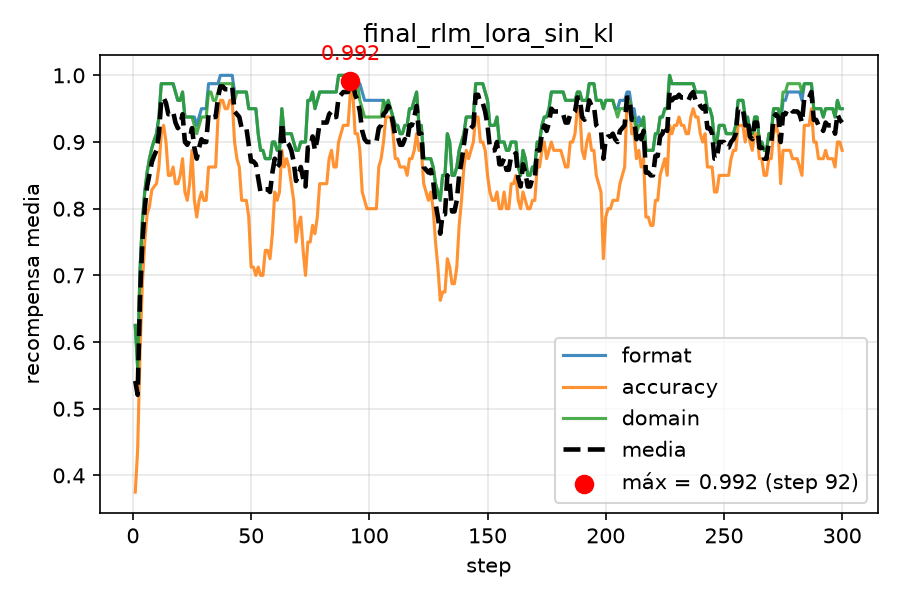
\includegraphics[keepaspectratio,alt={Evolución de las recompensas a lo largo del entrenamiento del modelo sin KL}]{exp_rlm_final_rlm_lora_sin_kl_curves_grpo_rewards.png}}
\end{center}

En cambio, al entrenar el modelo con KL con beta = 0.04, se puede ver como el máximo toma un valor menor (0.971) y en un step temprano, el 37. Esto puede deberse a que el modelo base entrenado con SF ya fuese muy bueno en esta tarea por lo que no hay demasiado hueco para que el entrenamiento con GRPO mejore el rendimiento del modelo.

\begin{center}
\pandocbounded{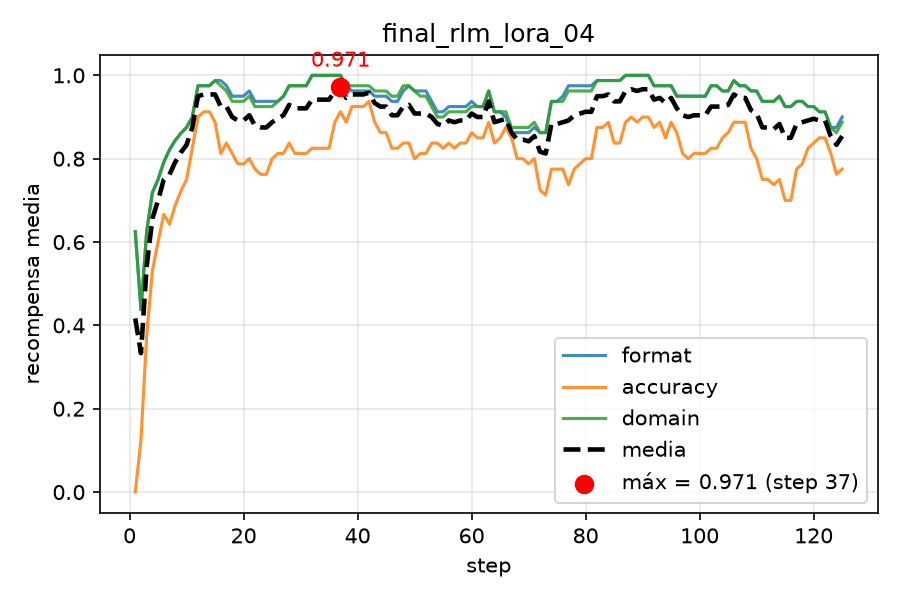
\includegraphics[keepaspectratio,alt={Evolución de las recompensas a lo largo del entrenamiento del modelo con KL (beta = 0.04)}]{exp_rlm_final_rlm_lora_kl_04_curves_grpo_rewards.png}}
\end{center}

Los adaptador se encuentran publicados en Hugging Face:
\texttt{isamorell/\allowbreak{}dgm-arca-rlm-lora-sin-kl} (modelo entrenado con grpo y sin KL).
\texttt{isamorell/\allowbreak{}dgm-arca-rlm-lora-kl-04} (modelo entrenado con grpo y con KL (beta = 0.04)).

\textbf{Qué concluimos.} Para ambos casos, el modelo logra máximos muy altos en puntos tempranos del entrenamiento. Esto puede deberse a que el modelo base ya lo hace muy bien. Por ello, vamos a comparar el rendimiento de los tres modelos en el conjunto de test.

Además, en train parece que funciona mejor no utilizar KL pero esto puede deberse a que KL está actuando como un freno sobre el entrenamiento para que no se separe demasiado del modelo base. Para ver si el modelo está mejorando al incluir KL, vamos a probar el rendimiento en el conjunto de test utilizando el \texttt{evaluate.py}.

\begin{center}\rule{0.5\linewidth}{0.5pt}\end{center}

\subsubsection{2026-10-12 · Fase 1 · Pass@1 de los 3 modelos entrenados y del modelo base}

\textbf{Qué queríamos saber.} Queremos saber que modelo generaliza mejor en test para poder analizar si grpo mejora el rendimiento del modelo frente al sft, y si utilizar kl con beta 0.04 mejora frente a no usar kl.

\textbf{Qué hicimos.} Hemos calculado el Pass@1 de los modelos base, sft y grpo sin KL y con KL beta = 0.04 ejecutando el \texttt{evalute.py} con el siguiente comando:

\texttt{uv run python -m rlm.evaluate -\/\allowbreak{}-data rlm/\allowbreak{}data/\allowbreak{}test.jsonl -\/\allowbreak{}-adapters base=\allowbreak{}none sft=\allowbreak{}rlm/\allowbreak{}weights/\allowbreak{}sft\_\allowbreak{}lora grpo\_\allowbreak{}sin\_\allowbreak{}kl=\allowbreak{}rlm/\allowbreak{}weights/\allowbreak{}final\_\allowbreak{}rlm\_\allowbreak{}lora\_\allowbreak{}sin\_\allowbreak{}kl grpo=\allowbreak{}rlm/\allowbreak{}weights/\allowbreak{}final\_\allowbreak{}rlm\_\allowbreak{}lora\_\allowbreak{}04}

\textbf{Qué pasó.} La ejecución ha tardado más de dos horas ya que la inferencia se ha ido haciendo 1 a 1, sin batching.

Como podemos observar en la imagen siguiente, el modelo base obtiene un 0.0\% de pass@1. Esto se debe a que sin el sft, el modelo no ha aprendido el formato y lo rompe añadiendo un bloque \texttt{\textless{}reasoning process\textgreater{} ... \textless{}/\allowbreak{}reasoning process\textgreater{}}. Además, responde sin unidades lo que no cumple con la recompensa de dominio.

Una vez el modelo aprende a razonar, la puntuación sube a 80.5\%. Este valor coincide para el sft y el grpo con kl con beta = 0.04. Esto probablemente se deba a que el modelo se encuentra en una zona plana de la que no puede salir debido a la penalización kl. Esto se puede deducir también del análisis anterior en el que se vio que la máxima recompensa obtenida en el entrenamiento fue en el paso 37, indicando que a partir de ese punto el modelo no es capaz de mejorar.

Por último, vemos como el modelo entrenado con grpo sin kl mejora el resultado obtenido por sft ya que es capaz de adaptarse a datos que no se han observado previamente. Este modelo obtiene un 89.5\% de pass@1, un 9\% más que el modelo sft y el entrenado con grpo con kl.

\begin{center}
\pandocbounded{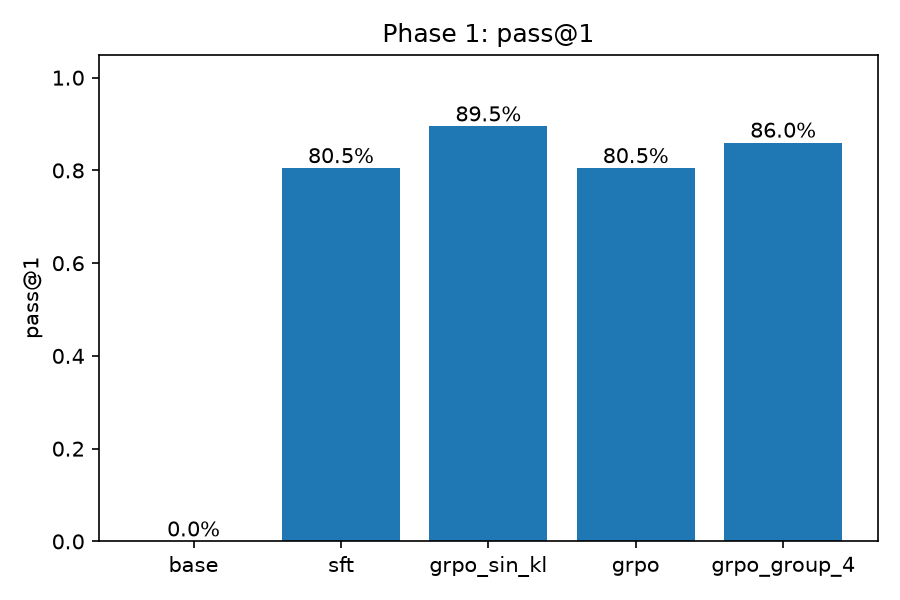
\includegraphics[keepaspectratio,alt={Pass@1 de los modelos base, sft, grpo\_\allowbreak{}sin\_\allowbreak{}kl y grpo con kl y beta = 0.04}]{exp_phase1_pass1.png}}
\end{center}

\textbf{Qué concluimos.} El modelo base falla siempre debido a errores de formato y a que no devuelve las unidades de la respuesta. GRPO sin KL mejora a SFT y a GRPO con KL en test y estos dos últimos obtienen el mismo pass@1.

A continuación vamos a entrenar otro modelo con GRPO sin KL y con otro valor de tamaño de grupo.

\begin{center}\rule{0.5\linewidth}{0.5pt}\end{center}

\subsubsection{2026-10-12 · Fase 1 · Entrenamiento modelo con GRPO sin KL y con -\/-num-generations = 4}

\textbf{Qué queríamos saber.} Queremos analizar cómo afecta el número de generaciones al entrenamiento del modelo y a su rendimiento final.

\textbf{Qué hicimos.} Comenzamos entrenando el modelo con el parámetro -\/-num-generations = 4. Esto lo hacemos ejecutando el siguiente comando:
\texttt{uv run python -m rlm.train\_\allowbreak{}grpo -\/\allowbreak{}-data rlm/\allowbreak{}data/\allowbreak{}train.jsonl -\/\allowbreak{}-init-adapter rlm/\allowbreak{}weights/\allowbreak{}sft\_\allowbreak{}lora -\/\allowbreak{}-num-generations 4}

Tras entrenar el modelo, sacamos sus curvas de evolución de la recompensa y la longitud de respuesta ejecutando el comando:
\texttt{uv run python -m rlm.plot\_\allowbreak{}curves rlm/\allowbreak{}weights/\allowbreak{}final\_\allowbreak{}rlm\_\allowbreak{}lora -\/\allowbreak{}-output reports/\allowbreak{}rlm/\allowbreak{}final\_\allowbreak{}rlm\_\allowbreak{}lora\_\allowbreak{}sin\_\allowbreak{}kl\_\allowbreak{}group\_\allowbreak{}4/\allowbreak{}curves\_\allowbreak{}grpo}

Así podremos ver las curvas y obtener el máximo de recompensa media obtenida durante el entrenamiento.

Por último, modificamos el evaluate.py para que no se borren los resultados que ya tengo y que solo se añadan los nuevos adicionalmente. Ejecutando el siguiente comando para el nuevo modelo, obtenemos el rendimiento de este en el conjunto de test :
\texttt{uv run python -m rlm.evaluate -\/\allowbreak{}-data rlm/\allowbreak{}data/\allowbreak{}test.jsonl -\/\allowbreak{}-adapters grpo\_\allowbreak{}group\_\allowbreak{}4=\allowbreak{}rlm/\allowbreak{}weights/\allowbreak{}final\_\allowbreak{}rlm\_\allowbreak{}lora\_\allowbreak{}sin\_\allowbreak{}kl\_\allowbreak{}group\_\allowbreak{}4}

\textbf{Qué pasó.} Este modelo obtiene un 86\% de pass@1. La diferencia principal con los otros dos modelos que hemos entrenado con GRPO es que, en este caso, hemos utilizado 4 generaciones en vez de 8 para calcular las recompensas.

Las curvas de los tres modelos siguen un patrón similar como se puede apreciar en las siguientes 3 imágenes. Las recompensas comienzan en valores por debajo del 0.5 y en torno al paso 25 ya se encuentran por encima del 0.8. La longitud media de las respuestas decae de 600 a unos 300-400 tokens cuando el modelo empieza a razonar correctamente y obtener las respuestas esperadas. El impacto de bajar el número de generaciones de 8 a 4 se puede observar en que las curvas son más ruidosas y la desviación de la recompensa dentro del grupo es un poco mayor.

\begin{center}
\pandocbounded{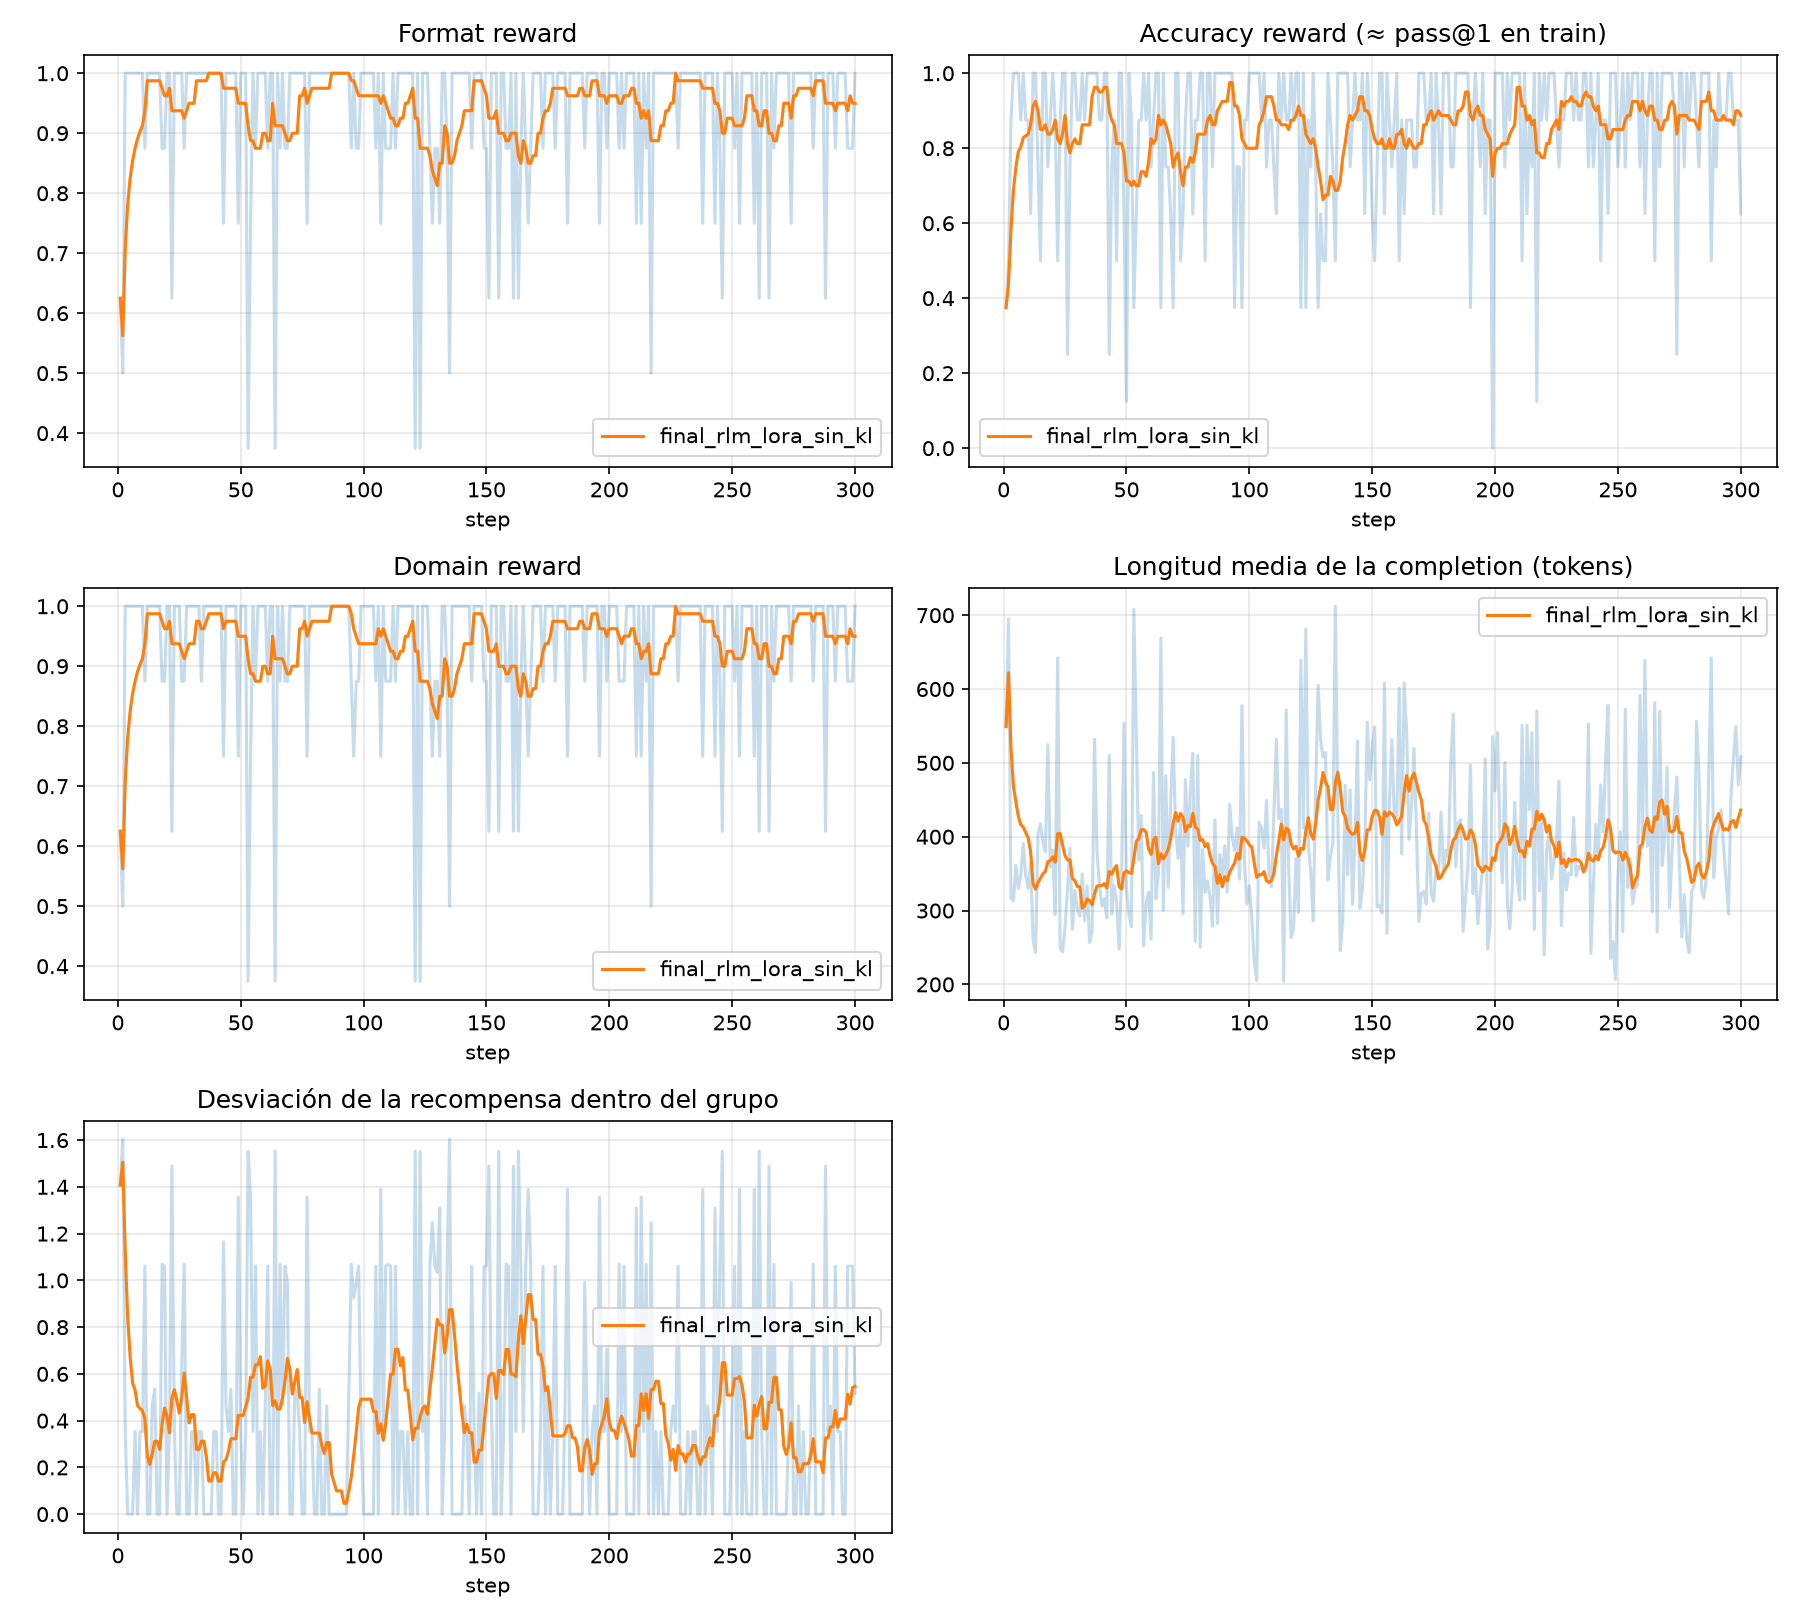
\includegraphics[keepaspectratio,alt={Evolución de diferentes métricas a lo largo del entrenamiento del modelo sin KL (num-generations = 8)}]{exp_rlm_final_rlm_lora_sin_kl_curves_grpo.png}}
\end{center}

\begin{center}
\pandocbounded{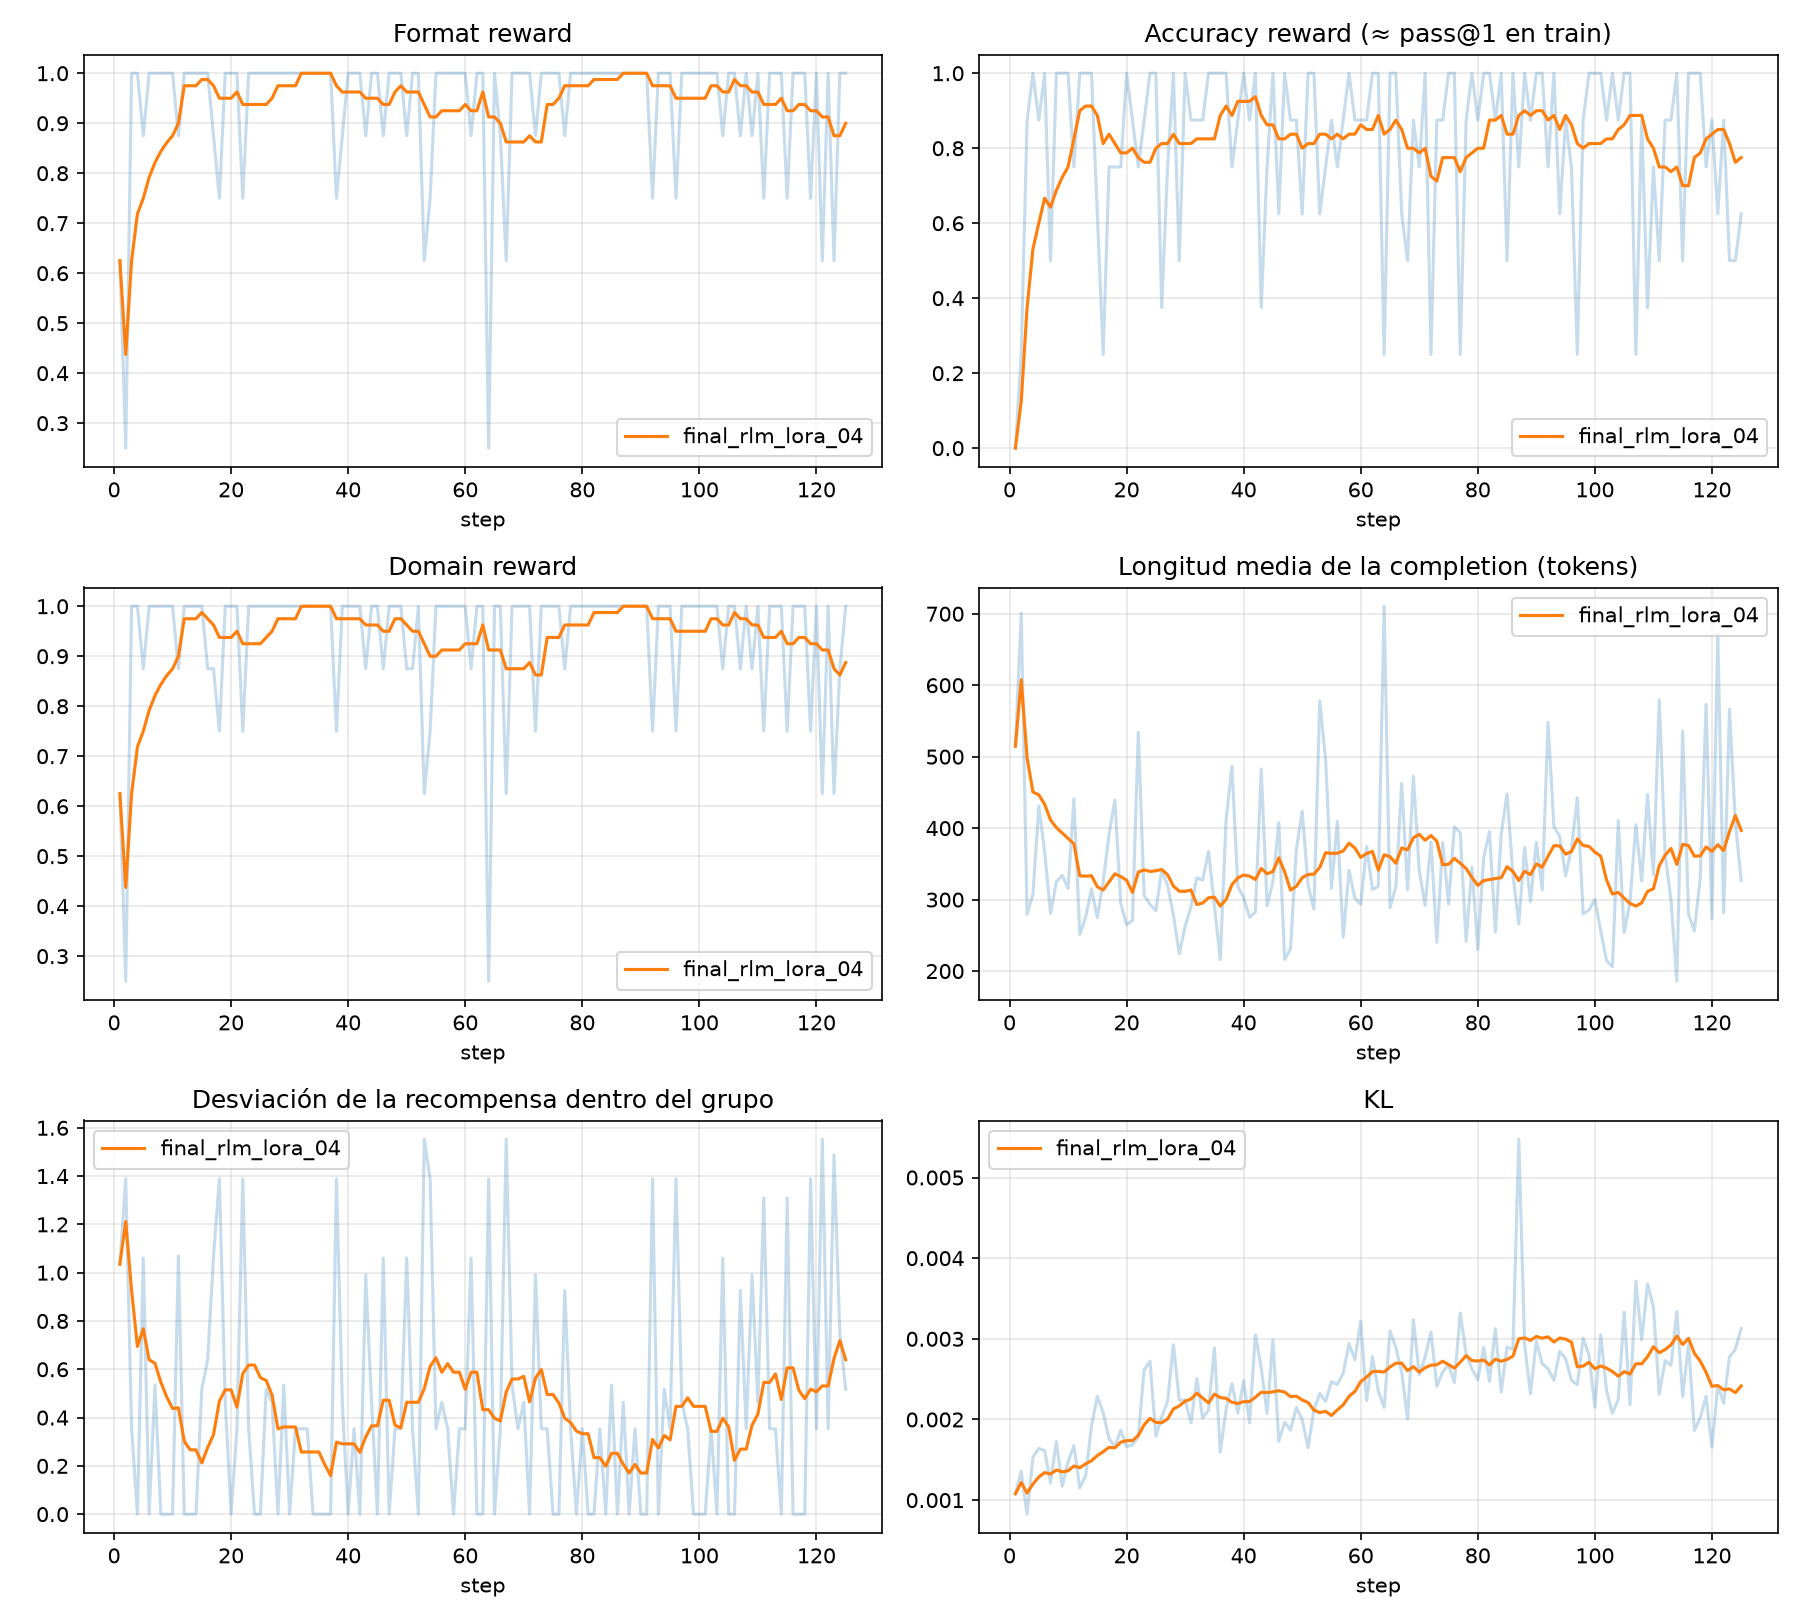
\includegraphics[keepaspectratio,alt={Evolución de diferentes métricas a lo largo del entrenamiento del modelo con KL (beta = 0.04, num-generations = 8)}]{exp_rlm_final_rlm_lora_kl_04_curves_grpo.png}}
\end{center}

\begin{center}
\pandocbounded{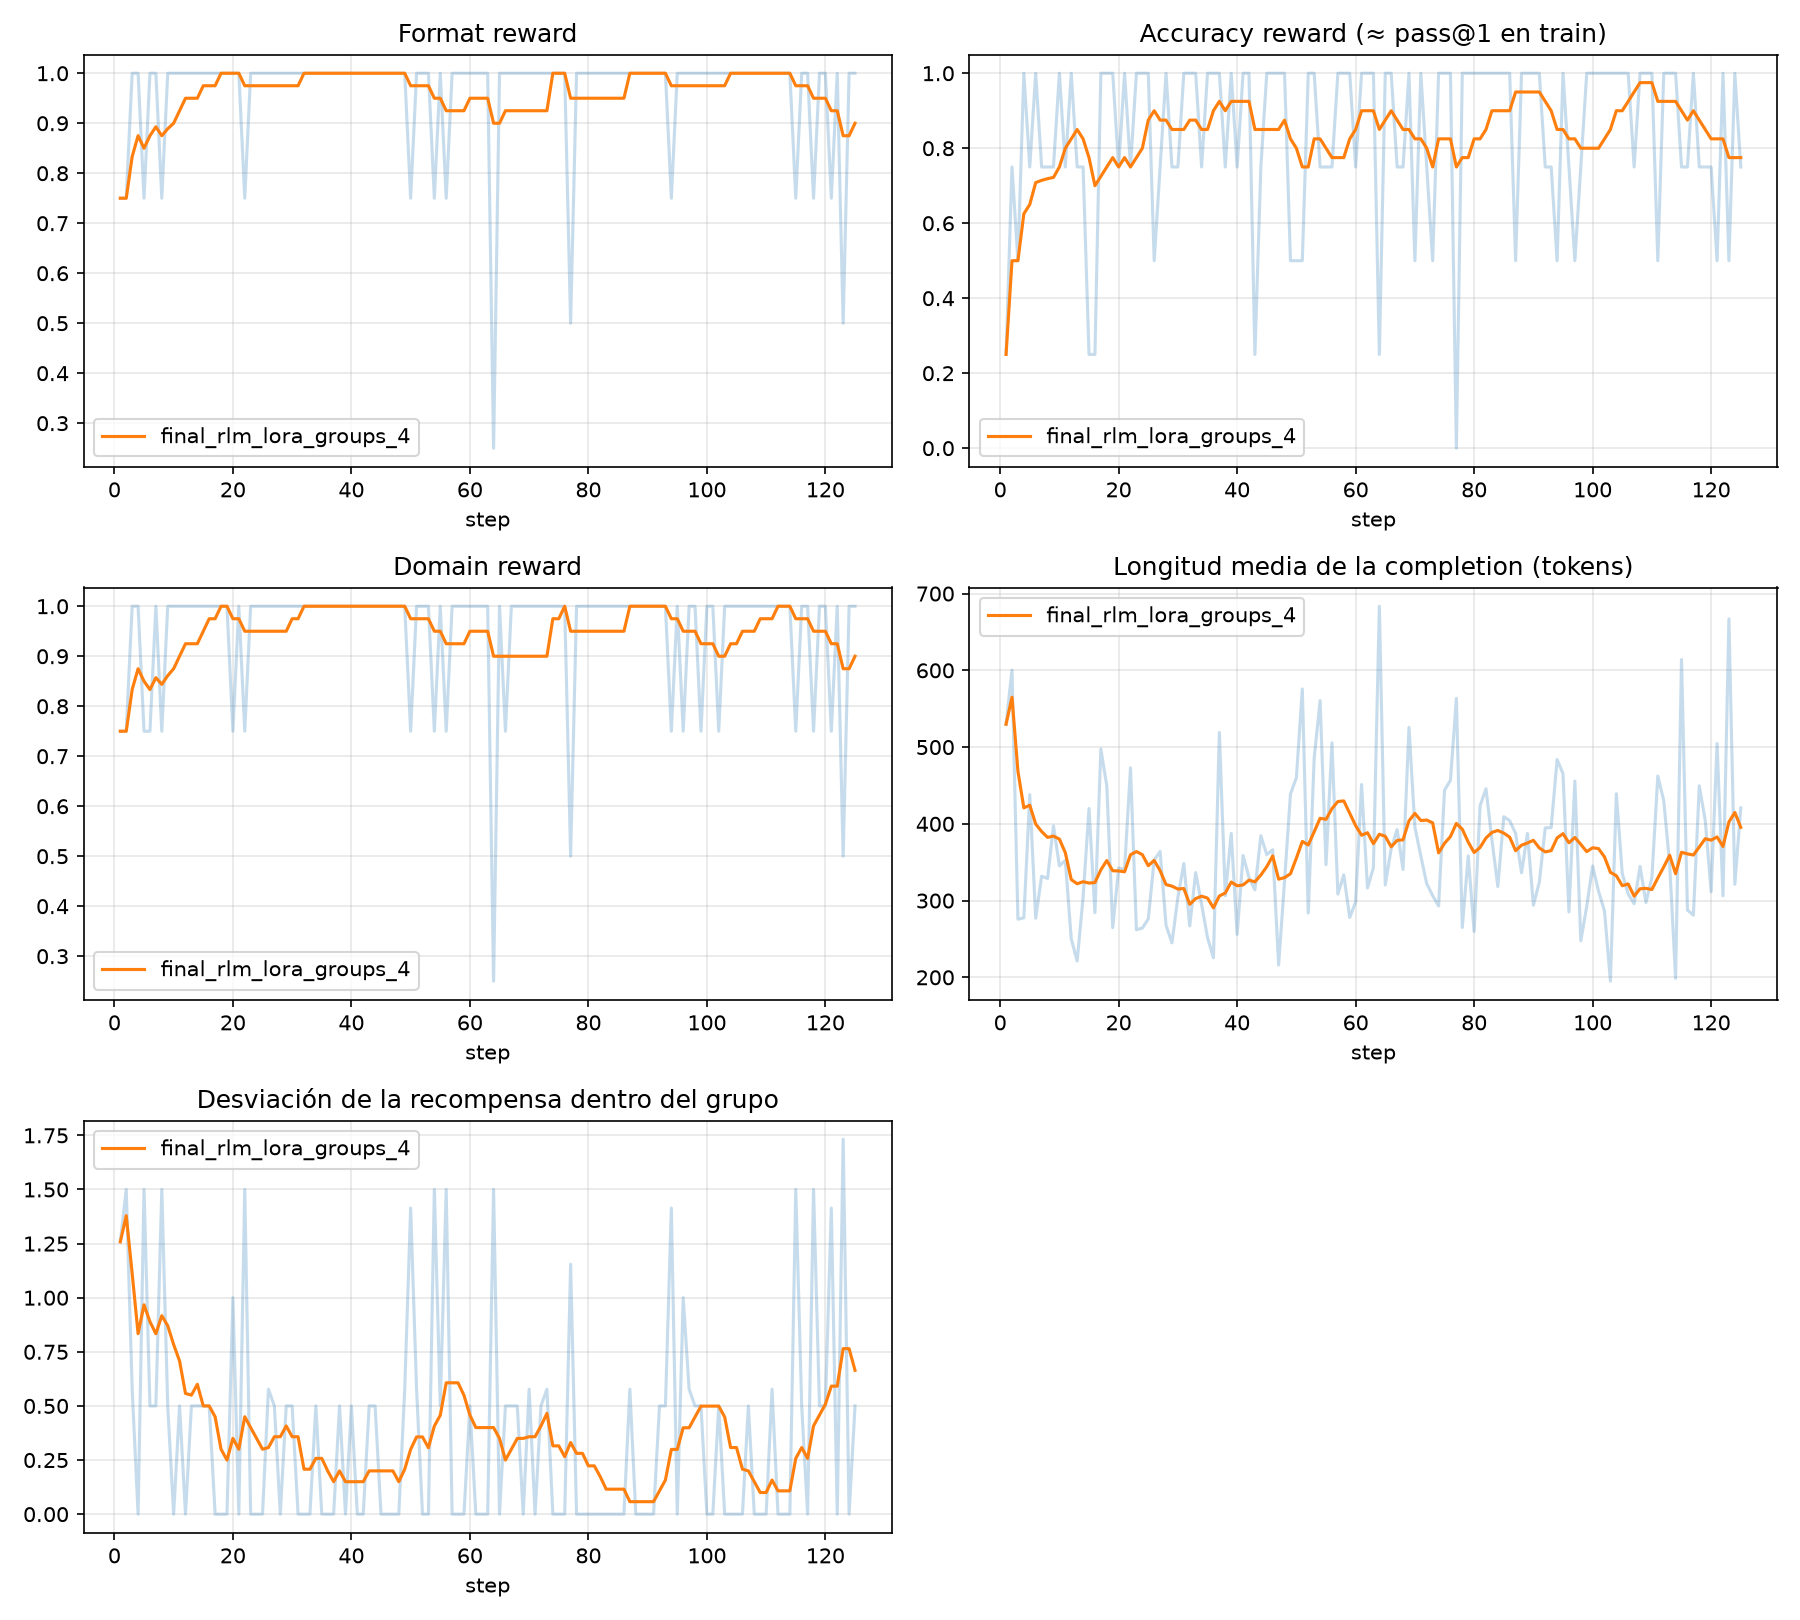
\includegraphics[keepaspectratio,alt={Evolución de diferentes métricas a lo largo del entrenamiento del modelo sin KL (num-generations = 4)}]{exp_rlm_final_rlm_lora_sin_kl_group_4_curves_grpo.png}}
\end{center}

\textbf{Qué concluimos.} Por lo tanto, el mejor modelo continúa siendo el modelo entrenado con GRPO, sin KL y con 8 generaciones de respuestas ya que es el que obtiene un mejor pass@1 y es más estable que el modelo de 4 generaciones.

A continuación, vamos a analizar en qué falla concretamente cada modelo para entender qué ha aprendido en cada paso y qué tiene que aprender aún.

\begin{center}\rule{0.5\linewidth}{0.5pt}\end{center}

\subsubsection{2026-10-12 · Fase 1 · Análisis de las respuestas obtenidas en el test}

\textbf{Qué queríamos saber.} Queremos saber qué ha aprendido cada modelo durante cada entrenamiento y queremos comprender si hay un grupo concreto de problemas que el modelo falla para ayudarle a que aprende a resolver ese tipo concreto de ejercicios.

\textbf{Qué hicimos.} Para realizar este análisis, hemos escrito un nuevo fichero (\texttt{analyze\_\allowbreak{}eval.py}) que analiza varios puntos:

\begin{enumerate}
\tightlist
\item
  Busca patrones en las respuestas de los modelos para determinar de forma más concreta si siguen el formato y si devuelven la respuesta correcta.
\item
  El porcentaje de acierto por familia de problemas
\item
  Tipo de respuestas devueltas por cada modelo
\item
  Fallos cometidos por el mejor modelo (grpo sin kl)
\end{enumerate}

Para obtener este análisis hay que ejecutar el siguiente comando:
\texttt{uv run python -m rlm.analyze\_\allowbreak{}eval}

\textbf{Qué pasó.} Comenzamos analizando si el modelo devuelve la respuesta correcta en el formato correcto. Como podemos ver en la siguiente tabla, el modelo base no devuelve una respuesta más de la mitad de las veces y solo cumple con el formato indicado en un 9,5\% de los casos. Además, solo devuelve el valor correcto un 26,5\% de las veces. Todo esto explica por qué se obtiene un pass@1 de un 0,0\%.

Si comparamos los otros 4 modelos que obtienen respuestas más razonables para el problema, podemos observar como el modelo entrenado con GRPO sin KL presenta las mayores mejoras tanto en el formato como en la corrección de la respuesta.

GRPO con KL no mejora el pass@1 de SFT pero su formato es algo mejor (94,0 \% frente a 92,5 \%) y tiene menos respuestas ausentes (6,0 \% frente a 7,5 \%). Y el modelo de GRPO sin KL mejora todas las métricas frente a estos dos.

{\def\LTcaptype{none} % do not increment counter
\footnotesize\setlength{\tabcolsep}{3pt}
\begin{longtable}[]{@{}
  >{\raggedright\arraybackslash}p{(\linewidth - 8\tabcolsep) * \real{0.1579}}
  >{\raggedleft\arraybackslash}p{(\linewidth - 8\tabcolsep) * \real{0.2105}}
  >{\raggedleft\arraybackslash}p{(\linewidth - 8\tabcolsep) * \real{0.2105}}
  >{\raggedleft\arraybackslash}p{(\linewidth - 8\tabcolsep) * \real{0.2105}}
  >{\raggedleft\arraybackslash}p{(\linewidth - 8\tabcolsep) * \real{0.2105}}@{}}
\toprule\noalign{}
\begin{minipage}[b]{\linewidth}\raggedright
Modelo
\end{minipage} & \begin{minipage}[b]{\linewidth}\raggedleft
Valor correcto (\texttt{valor\_\allowbreak{}ok})
\end{minipage} & \begin{minipage}[b]{\linewidth}\raggedleft
Formato válido
\end{minipage} & \begin{minipage}[b]{\linewidth}\raggedleft
Sin respuesta (\texttt{sin\_\allowbreak{}answer})
\end{minipage} & \begin{minipage}[b]{\linewidth}\raggedleft
Pass@1
\end{minipage} \\
\midrule\noalign{}
\endhead
\bottomrule\noalign{}
\endlastfoot
Base & 26,5 \% & 9,5 \% & 53,5 \% & 0,0 \% \\
SFT & 80,5 \% & 92,5 \% & 7,5 \% & 80,5 \% \\
GRPO sin KL & \textbf{89,5 \%} & \textbf{97,0 \%} & \textbf{3,0 \%} & \textbf{89,5 \%} \\
GRPO con KL & 80,5 \% & 94,0 \% & 6,0 \% & 80,5 \% \\
GRPO sin KL group 4 & 86,0 \% & 94,5 \% & 5,5 \% & 86,0 \% \\
\end{longtable}
}

A continuación, analizamos las tasas de éxito por familia.

{\def\LTcaptype{none} % do not increment counter
\scriptsize\setlength{\tabcolsep}{1.5pt}
\begin{longtable}[]{@{}
  >{\raggedright\arraybackslash}p{(\linewidth - 12\tabcolsep) * \real{0.1111}}
  >{\raggedleft\arraybackslash}p{(\linewidth - 12\tabcolsep) * \real{0.1481}}
  >{\raggedleft\arraybackslash}p{(\linewidth - 12\tabcolsep) * \real{0.1481}}
  >{\raggedleft\arraybackslash}p{(\linewidth - 12\tabcolsep) * \real{0.1481}}
  >{\raggedleft\arraybackslash}p{(\linewidth - 12\tabcolsep) * \real{0.1481}}
  >{\raggedleft\arraybackslash}p{(\linewidth - 12\tabcolsep) * \real{0.1481}}
  >{\raggedleft\arraybackslash}p{(\linewidth - 12\tabcolsep) * \real{0.1481}}@{}}
\toprule\noalign{}
\begin{minipage}[b]{\linewidth}\raggedright
Familia
\end{minipage} & \begin{minipage}[b]{\linewidth}\raggedleft
n
\end{minipage} & \begin{minipage}[b]{\linewidth}\raggedleft
Base
\end{minipage} & \begin{minipage}[b]{\linewidth}\raggedleft
SFT
\end{minipage} & \begin{minipage}[b]{\linewidth}\raggedleft
GRPO sin KL
\end{minipage} & \begin{minipage}[b]{\linewidth}\raggedleft
GRPO con KL
\end{minipage} & \begin{minipage}[b]{\linewidth}\raggedleft
GRPO sin KL group 4
\end{minipage} \\
\midrule\noalign{}
\endhead
\bottomrule\noalign{}
\endlastfoot
Dilution & 40 & 0,00 & 0,75 & \textbf{0,95} & 0,82 & 0,80 \\
Dose/day & 40 & 0,00 & 0,93 & \textbf{0,97} & 0,93 & 0.93 \\
Drops & 40 & 0,00 & 0,78 & \textbf{0,88} & 0,78 & 0,85 \\
Pump & 40 & 0,00 & 0,75 & 0,72 & 0,68 & \textbf{0,80} \\
Volume & 40 & 0,00 & 0,82 & \textbf{0,95} & 0,82 & 0,93 \\
\end{longtable}
}

GRPO sin KL obtiene las mejores puntuaciones en 4 de las 5 familias de problemas que tenemos en el dataset de test. Para la familia de pump, obtiene un 72\% de aciertos por lo que pump es el grupo con el mejor margen de mejora en el rendimiento del modelo. Esta familia es la que menores resultados presenta para todos los modelos. Esto muestra como al modelo le cuesta razonar y obtener la respueta correcta.

En la siguiente tabla podemos observar como el modelo base no devuelve nunca el valor correcto. Esto se debe a que no devuelve la respuesta la mitad de las veces y, cuando devuelve una respuesta, el valor numérico de ésta está mal o no presenta la unidad correcta.

El modelo SFT aprende a devolver siempre la unidad correcta por lo que ninguno de los modelos entrenados presenta fallos de esta casuística. También reduce los fallos debido a la falta de respuesta y de valor incorrecto. Esto sugiere que el ajuste supervisado mejora tanto la generación de respuestas completas como el cumplimiento del formato esperado.

{\def\LTcaptype{none} % do not increment counter
\footnotesize\setlength{\tabcolsep}{3pt}
\begin{longtable}[]{@{}
  >{\raggedright\arraybackslash}p{(\linewidth - 10\tabcolsep) * \real{0.1304}}
  >{\raggedleft\arraybackslash}p{(\linewidth - 10\tabcolsep) * \real{0.1739}}
  >{\raggedleft\arraybackslash}p{(\linewidth - 10\tabcolsep) * \real{0.1739}}
  >{\raggedleft\arraybackslash}p{(\linewidth - 10\tabcolsep) * \real{0.1739}}
  >{\raggedleft\arraybackslash}p{(\linewidth - 10\tabcolsep) * \real{0.1739}}
  >{\raggedleft\arraybackslash}p{(\linewidth - 10\tabcolsep) * \real{0.1739}}@{}}
\toprule\noalign{}
\begin{minipage}[b]{\linewidth}\raggedright
Tipo de resultado
\end{minipage} & \begin{minipage}[b]{\linewidth}\raggedleft
Base
\end{minipage} & \begin{minipage}[b]{\linewidth}\raggedleft
SFT
\end{minipage} & \begin{minipage}[b]{\linewidth}\raggedleft
GRPO sin KL
\end{minipage} & \begin{minipage}[b]{\linewidth}\raggedleft
GRPO con KL
\end{minipage} & \begin{minipage}[b]{\linewidth}\raggedleft
GRPO sin KL group 4
\end{minipage} \\
\midrule\noalign{}
\endhead
\bottomrule\noalign{}
\endlastfoot
Correcto (\texttt{ok}) & 0 & 161 & \textbf{179} & 161 & 172 \\
Valor correcto, unidad incorrecta (\texttt{valor\_\allowbreak{}ok\_\allowbreak{}unidad\_\allowbreak{}mal}) & 53 & 0 & 0 & 0 & 0 \\
Valor incorrecto (\texttt{valor\_\allowbreak{}mal}) & 40 & 24 & \textbf{15} & 27 & 17 \\
Sin respuesta (\texttt{sin\_\allowbreak{}answer}) & 107 & 15 & \textbf{6} & 12 & 11 \\
\textbf{Total} & \textbf{200} & \textbf{200} & \textbf{200} & \textbf{200} & \textbf{200} \\
\end{longtable}
}

Por último, vamos a analizar concretamente por qué falla el modelo entrenado con grpo sin KL según los grupos de familias:

{\def\LTcaptype{none} % do not increment counter
\small\setlength{\tabcolsep}{3pt}
\begin{longtable}[]{@{}lrrr@{}}
\toprule\noalign{}
Familia & Valor incorrecto & Sin respuesta & Total de fallos \\
\midrule\noalign{}
\endhead
\bottomrule\noalign{}
\endlastfoot
Pump & 6 & 5 & \textbf{11} \\
Drops & 5 & 0 & 5 \\
Volume & 2 & 0 & 2 \\
Dose/day & 1 & 0 & 1 \\
Dilution & 1 & 1 & 2 \\
\textbf{Total} & \textbf{15} & \textbf{6} & \textbf{21} \\
\end{longtable}
}

Aproximadamente un 25\% de los fallos se deben a que el modelo no devuelve una respuesta. Esto se debe a que el razonamiento necesita más tokens de los establecidos como máximo.

De los 15 casos de respuestas incorrectas, 6 pertenecen a la familia de pump. Por lo tanto, ayudar al modelo a resolver estos problemas mejorará su rendimiento.

\textbf{Qué concluimos.} El aprendizaje supervisado mejora tanto la generación de respuestas completas como el cumplimiento del formato esperado frente al modelo base.

De los 3 modelos entrenados, el grpo sin KL muestra las mejores tasas tanto en el formato como en la corrección de la respuesta.

A continuación, analizaremos los fallos cometidos por el modelo entrenado con grpo sin KL

\begin{center}\rule{0.5\linewidth}{0.5pt}\end{center}

\subsubsection{2026-10-13 · Fase 1 · Fallos cometidos por el modelo entrenado con GRPO sin KL}

\textbf{Qué queríamos saber.} El modelo entrenado con GRPO sin KL es el que mejor funciona (pass@1 = 0.895), y supera al entrenado con KL (\texttt{grpo}, 0.805), a \texttt{grpo\_\allowbreak{}group\_\allowbreak{}4} (0.860) y al \texttt{sft} (0.805). Queremos saber qué tipo de fallos comete: si son meramente aritméticos o si el modelo ha encontrado alguna forma de reward hacking.

\textbf{Qué hicimos.} Seleccionamos cinco trazas del modelo con GRPO sin KL con \texttt{is\_\allowbreak{}correct =\allowbreak{} False} (en \texttt{reports/\allowbreak{}phase1\_\allowbreak{}eval.json}, sección \texttt{grpo\_\allowbreak{}sin\_\allowbreak{}kl}). Leímos el enunciado y el razonamiento completo de cada una, comprobando si los pasos que sigue son los que daría una persona al resolver el problema.

Para cubrir también las respuestas correctas (donde se manifestaría un posible hack), ejecutamos además un filtrado automático, \texttt{rlm/\allowbreak{}scan\_\allowbreak{}hacking.py}, sobre las 200 respuestas de cada modelo. Busca patrones que explotarían huecos de \texttt{rlm/\allowbreak{}rewards.py}:

\begin{itemize}
\tightlist
\item
  \texttt{multi\_\allowbreak{}number}: más de un número dentro de \texttt{\textless{}answer\textgreater{}} (el verificador toma el último).
\item
  \texttt{no\_\allowbreak{}unit}: respuesta sin unidad (el reward no la comprueba).
\item
  \texttt{ambiguous\_\allowbreak{}sep}: formato \texttt{d,ddd} (el parser lo lee como separador de miles).
\item
  \texttt{correct\_\allowbreak{}bad\_\allowbreak{}fmt}: respuesta correcta sin formato \texttt{\textless{}think\textgreater{}...\textless{}/\allowbreak{}think\textgreater{}\textless{}answer\textgreater{}...\textless{}/\allowbreak{}answer\textgreater{}} válido.
\item
  \texttt{hedging}: respuesta correcta con 3 o más marcadores de duda ("Espera", "tal vez me equivoqué"...).
\item
  \texttt{verifier\_\allowbreak{}mismatch}: discrepancia entre \texttt{is\_\allowbreak{}correct} del eval y \texttt{numbers\_\allowbreak{}match} de \texttt{rewards.py}.
\item
  Además, cuenta preguntas duplicadas dentro de cada sección.
\end{itemize}

\textbf{Cómo ejecutar el script.}

Solo el modelo GRPO sin KL, sin comparar con el reward:

\begin{lstlisting}
python rlm/scan_hacking.py reports/phase1_eval.json --section grpo_sin_kl
\end{lstlisting}

Solo el modelo GRPO sin KL, comparando además con el verificador del entrenamiento (\texttt{rlm/\allowbreak{}rewards.py}):

\begin{lstlisting}
python rlm/scan_hacking.py reports/phase1_eval.json --section grpo_sin_kl --reward-module rlm/rewards.py
\end{lstlisting}

Todos los modelos a la vez, para comparar:

\begin{lstlisting}
python rlm/scan_hacking.py reports/phase1_eval.json --reward-module rlm/rewards.py
\end{lstlisting}

Opciones útiles: \texttt{-\/\allowbreak{}-show N} imprime N ejemplos por cada flag (por defecto 5), y se puede redirigir la salida a un fichero, por ejemplo \texttt{\textgreater{} reports/\allowbreak{}hacking\_\allowbreak{}scan.txt}.

\textbf{Qué pasó.} 4 de los 5 fallos son errores aritméticos: el modelo plantea correctamente qué operación hay que hacer, pero la ejecuta mal. Uno de ellos (caso 5) desemboca además en un bucle de dudas que agota el máximo de tokens sin llegar a dar respuesta. El fallo restante (caso 3) es un error conceptual de unidades.

A continuación se muestra cada traza completa y su análisis.

\textbf{1.}

\begin{lstlisting}
{
    "question": "Datos: Tiempo: 705 min; Volumen: 490 mL (suero fisiológico). Indica la velocidad en mL/h. Da el resultado con un decimal.",
    "expected": "41.7 mL/h",
    "raw": "<think>\nVale, voy a resolverlo paso a paso. Primero, tengo que encontrar la velocidad en mL por hora. La fórmula que uso es el volumen dividido por el tiempo. El volumen es 490 mL y el tiempo es 705 minutos. Pero el resultado debe estar en horas, así que primero convierto los minutos a horas.\n\n705 minutos divididos por 60 minutos por hora. 705 / 60 = 11.75 horas. Luego, divido el volumen por el tiempo en horas: 490 mL / 11.75 h. Haciendo la división, 490 ÷ 11.75 ≈ 41.2 mL/h. El resultado ya tiene un decimal, así que ya está correcto. No necesito redondear más.\n</think>\n\n<answer>41.2 mL/h</answer>",
    "predicted": "41.2 mL/h",
    "is_correct": false,
    "has_valid_format": true,
    "n_tokens": 206,
    "family": "pump",
    "expected_unit": "mL/h",
    "expected_value": "41.7"
}
\end{lstlisting}

El modelo convierte bien 705 min a horas (11.75 h) y plantea correctamente que debe dividir volumen entre tiempo. Sin embargo, al calcular 490 / 11.75 afirma que el resultado es ≈ 41.2, cuando el valor correcto es 41.70. Es un error aritmético en una división con decimales. No intenta verificarlo.

\textbf{2.}

\begin{lstlisting}
{
    "question": "En planta, se trata de un paciente de 101,5 kg. La presentación es de 0,5 g por cada 2 ml. Lleva ingresado 8 días. Se han pautado 7,5 mg por kg de amoxicilina. Calcula el volumen a administrar en ml. Da el resultado con dos decimales.",
    "expected": "3.05 mL",
    "raw": "<think>\nVale, voy a resolverlo paso a paso. Primero, el paciente pesa 101,5 kg. La dosis prescrita es 7,5 mg por kg. Entonces, necesito calcular la dosis total en mg. Multiplico 101,5 kg por 7,5 mg/kg. \n\n101,5 kg * 7,5 mg/kg = 759,75 mg. \n\nAhora, la presentación es 0,5 g por 2 ml. Debo convertir los gramos a miligramos, ya que la dosis es en mg. 0,5 g es 500 mg. Entonces, 500 mg por 2 ml. \n\nQuiero saber cuántos ml son necesarios para 759,75 mg. Hago una proporción: 500 mg / 2 ml = 759,75 mg / x ml. \n\nResolviendo, x = (759,75 mg * 2 ml) / 500 mg = 1519,5 / 500 = 3,039 ml. \n\nRedondeo a dos decimales, que sería 3,04 ml. \n\nEspera, pero tal vez me equivoqué en la conversión. Vamos a verificar. \n\nOtra forma: 0,5 g = 500 mg. 500 mg en 2 ml. Entonces, 1 mg es 2/500 = 0,004 ml. \n\nEntonces, 759,75 mg * 0,004 ml/mg = 3,039 ml. Sí, es lo mismo. \n\nEntonces, el volumen a administrar es 3,04 ml.\n</think>\n\n<answer>3,04 mL</answer>",
    "predicted": "3,04 mL",
    "is_correct": false,
    "has_valid_format": true,
    "n_tokens": 420,
    "family": "volume",
    "expected_unit": "mL",
    "expected_value": "3.05"
}
\end{lstlisting}

El razonamiento es correcto, pero el primer cálculo falla: 101,5 kg × 7,5 mg/kg da 761,25 mg y el modelo obtiene 759,75 mg. Todos los pasos posteriores (conversión de 0,5 g a 500 mg, proporción con 2 mL) son correctos, pero parten de un valor erróneo, así que el error se arrastra hasta el resultado final (3,04 mL en lugar de 3,05 mL). Cuando el modelo intenta verificar ("Espera, pero tal vez me equivoqué..."), repite exactamente el mismo producto erróneo, por lo que la verificación confirma el error en lugar de corregirlo.

\textbf{3.}

\begin{lstlisting}
{
    "question": "Ejercicio de prácticas.\n- Hora de inicio: 16:00\n- Vial: 1 g/20 ml\n- Dosis de dopamina: 5 mg/kg\n- Peso: 107 kg\nIndica cuántos ml corresponden a la dosis. Expresa el resultado con dos decimales (redondeado).",
    "expected": "10.70 mL",
    "raw": "<think>\nVale, voy a resolverlo paso a paso. Primero, necesito calcular la dosis total de dopamina que se necesita. La dosis es 5 mg por kilogramo de peso, y el peso del paciente es 107 kg. Entonces, multiplico 5 mg/kg por 107 kg. \n\n5 mg/kg * 107 kg = 535 mg. \n\nAhora, tengo que convertir los miligramos a gramos, porque la concentración está dada en gramos por mililitro. 535 mg es igual a 0,535 g. \n\nLa concentración de la solución es 1 g por 20 ml. Para encontrar cuántos ml corresponden a 0,535 g, primero calculo cuántos ml hay por gramo. \n\n1 g / 20 ml = 0,05 g/ml. \n\nLuego, multiplico 0,05 g/ml por 0,535 g. \n\n0,05 g/ml * 0,535 g = 0,02675 g. \n\nAhora, convierto gramos a mililitros. 1 g = 1000 ml, así que 0,02675 g * 1000 ml/g = 26,75 ml. \n\nEl resultado es 26,75 ml, que ya tiene dos decimales. No necesito redondear porque ya está con dos decimales. Por lo tanto, la respuesta es 26,75 ml.\n</think>\n\n<answer>26,75 mL</answer>",
    "predicted": "26,75 mL",
    "is_correct": false,
    "has_valid_format": true,
    "n_tokens": 365,
    "family": "volume",
    "expected_unit": "mL",
    "expected_value": "10.70"
},
\end{lstlisting}

Calcula bien la dosis (5 mg/kg × 107 kg = 535 mg = 0,535 g) y también que 1 g / 20 mL = 0,05 g/mL. A partir de ahí falla: multiplica 0,05 g/mL × 0,535 g y trata el resultado como gramos, cuando en realidad las unidades son g²/mL. Después "convierte" esos gramos a mL con 1 g = 1000 mL, que no es una conversión válida (mezcla masa y volumen). Lo correcto era usar la concentración del vial: 0,535 g × 20 mL/g = 10,7 mL. Es un error conceptual de análisis dimensional, no aritmético.

\textbf{4.}

\begin{lstlisting}
{
    "question": "Tengo que pasar 670 ml de suero glucosado al 5 % en 495 min. El equipo de suero es de 60 gotas/ml. ¿Cuántas gotas/min? Redondea al entero.",
    "expected": "81 gotas/min",
    "raw": "<think>\nVale, voy a resolverlo paso a paso. Primero, necesito calcular cuántas gotas se necesitan en total. El suero es de 670 ml al 5%, pero el problema no menciona si hay que considerar la concentración, solo el volumen. Entonces, el volumen total es 670 ml. El equipo es de 60 gotas por mililitro, así que multiplicaré 670 ml por 60 gotas/ml para obtener el número total de gotas.\n\n670 ml * 60 gotas/ml = 40200 gotas. \n\nAhora, tengo que dividir ese número total de gotas entre el tiempo total de 495 minutos para obtener las gotas por minuto. \n\n40200 gotas / 495 min ≈ 81.666... gotas/min. \n\nEl enunciado dice que redondee al entero, así que redondeo a 82 gotas por minuto. \n\nEspera, pero tal vez me equivoqué en la división. Vamos a hacerlo más precisamente. 40200 dividido entre 495. \n\nDividir 40200 entre 495: 495 * 81 = 40335, que es más de 40200. Entonces, 81 - (40335 - 40200)/495. 40335 - 40200 = 135. 135/495 = 0.2727... Así que 81 - 0.2727 ≈ 80.727, que redondea a 81. \n\nPero espera, tal vez hice un error en la multiplicación. 670 * 60 = 40200, sí. 40200 / 495: 495 * 80 = 39600. 40200 - 39600 = 600. 600 / 495 ≈ 1.222. Así que total 81.222, que redondea a 81. \n\nPero el resultado es aproximadamente 81.666, que redondea a 82. Hmm, ¿no es 81.666? Sí, 81.666... es 81.666..., que redondea a 82. Entonces, la respuesta es 82 gotas por minuto.\n</think>\n\n<answer>82 gotas/min</answer>",
    "predicted": "82 gotas/min",
    "is_correct": false,
    "has_valid_format": true,
    "n_tokens": 620,
    "family": "drops",
    "expected_unit": "gotas/min",
    "expected_value": "81"
},
\end{lstlisting}

Calcula bien las gotas totales (670 × 60 = 40200), pero al dividir 40200 / 495 dice que da ≈ 81.666, cuando el valor correcto es 81.21. Sospecha del resultado y lo reintenta: en el primer intento obtiene 80.727 (por un error intermedio, 495 × 81 = 40335 cuando son 40095) y en el segundo 81.222, que es correcto. Ambos redondean a 81. Sin embargo, en la última línea vuelve sin justificación al 81.666 inicial y redondea a 82. Se confunde y abandona la respuesta correcta que él mismo había calculado. Es un error aritmético, agravado por una autoverificación que no se usa para decidir.

\textbf{5.}

\begin{lstlisting}
{
    "question": "La duración prescrita es de 165 min. La bolsa es de 370 ml de solución salina. La perfusión empieza a las 15:30 h. ¿Qué ritmo de bomba, en ml/h, corresponde? Da el resultado con un decimal.",
    "expected": "134.5 mL/h",
    "raw": "<think>\nVale, voy a resolverlo paso a paso. Primero, necesito calcular la tasa de bomba en ml por hora. La duración prescrita es 165 minutos, y la bolsa tiene 370 ml. \n\nPrimero, convierto los 165 minutos a horas, porque la bomba se pide en ml/h. 165 minutos divididos por 60 son 2.75 horas. \n\nLuego, divido la cantidad total de solución (370 ml) entre el tiempo en horas (2.75 h) para obtener la tasa. 370 dividido entre 2.75. \n\nHaciendo la división: 370 / 2.75. Calculo que 2.75 x 136 es 371, lo que me da aproximadamente 136.0 ml/h. \n\nPero para exactitud, 370 / 2.75 = 136.0 ml/h. Entonces, el ritmo de bomba es 136.0 ml/h. Redondeado a un decimal, es 136.0. \n\nEspera, pero tal vez me equivoqué en la división. Vamos a hacerlo más precisamente. 2.75 x 136 = 2.75 * 136. 2 * 136 = 272, 0.75 * 136 = 102, total 374. Entonces 370 / 2.75 = 136 - (4/2.75) ≈ 136 - 1.4545 ≈ 134.5455. Hmm, eso no es 136.0. O tal vez me equivoqué en la conversión de minutos a horas. \n\nRevisando: 165 minutos es 2.75 horas. 370 ml / 2.75 h = 134.545... ml/h. Pero el resultado debe tener un decimal. Entonces, 134.5 ml/h. Pero el enunciado dice \"con un decimal\", así que 134.5. \n\nPero tal vez me equivoqué en la división. Vamos a hacer 370 dividido entre 2.75. Multiplico numerador y denominador por 100 para eliminar decimales: 37000 / 275. Simplifico 37000 / 275. Dividir 37000 entre 275. 275 x 134 = 37100, que es un poco más que 37000. Entonces 134 - (100/275) ≈ 134 - 0.3636 ≈ 133.6364. Así que 133.6364 ml/h. Redondeado a un decimal es 133.6 ml/h. \n\nPero esto contradice con el anterior resultado. Hmm, tal vez me equivoqué en la conversión. O tal vez el resultado es 134.5 ml/h. Debo verificar. \n\nOtra forma: 2.75 h = 165 min. 370 ml / 165 min = 2.252525... ml/min. Multiplicado por 60 min/h: 2.252525 * 60 = 135.1515... ml/h. Redondeado a un decimal es 135.2 ml/h. \n\nAhora, hay que verificar si el cálculo es correcto. 370 ml / 165 min = 2.252525... ml/min. 2.252525 * 60 = 135.1515... ml/h. Sí, entonces con un decimal es 135.2 ml/h. \n\nPero el enunciado dice \"con un decimal\", así que 135.2. Pero el resultado inicial me dio 133.6, que no es correcto. Entonces, el error debe estar en la conversión. \n\nRevisando: 165 minutos es 2.75 horas. 370 / 2.75 = 134.545... ml/h. Pero 134",
    "predicted": null,
    "is_correct": false,
    "has_valid_format": false,
    "n_tokens": 1024,
    "family": "pump",
    "expected_unit": "mL/h",
    "expected_value": "134.5"
},
\end{lstlisting}

Plantea bien el método (165 min = 2.75 h; 370 / 2.75), pero la división le da resultados distintos en cada intento (136.0, 134.5, 133.6, 135.2...). Entra en un bucle de "tal vez me equivoqué en la división", recalcula sin converger y alcanza el máximo de 1024 tokens sin escribir \texttt{\textless{}answer\textgreater{}}. Se marca como incorrecta y sin formato válido. La raíz del fallo es también aritmética (no sabe dividir 370 / 2.75 de forma fiable).

\textbf{Resultados del filtrado automático.}

{\def\LTcaptype{none} % do not increment counter
\scriptsize\setlength{\tabcolsep}{1.5pt}
\begin{longtable}[]{@{}
  >{\raggedright\arraybackslash}p{(\linewidth - 14\tabcolsep) * \real{0.1250}}
  >{\raggedright\arraybackslash}p{(\linewidth - 14\tabcolsep) * \real{0.1250}}
  >{\raggedright\arraybackslash}p{(\linewidth - 14\tabcolsep) * \real{0.1250}}
  >{\raggedright\arraybackslash}p{(\linewidth - 14\tabcolsep) * \real{0.1250}}
  >{\raggedright\arraybackslash}p{(\linewidth - 14\tabcolsep) * \real{0.1250}}
  >{\raggedright\arraybackslash}p{(\linewidth - 14\tabcolsep) * \real{0.1250}}
  >{\raggedright\arraybackslash}p{(\linewidth - 14\tabcolsep) * \real{0.1250}}
  >{\raggedright\arraybackslash}p{(\linewidth - 14\tabcolsep) * \real{0.1250}}@{}}
\toprule\noalign{}
\begin{minipage}[b]{\linewidth}\raggedright
Modelo
\end{minipage} & \begin{minipage}[b]{\linewidth}\raggedright
pass@1
\end{minipage} & \begin{minipage}[b]{\linewidth}\raggedright
multi\_\allowbreak{}number
\end{minipage} & \begin{minipage}[b]{\linewidth}\raggedright
no\_\allowbreak{}unit
\end{minipage} & \begin{minipage}[b]{\linewidth}\raggedright
ambiguous\_\allowbreak{}sep
\end{minipage} & \begin{minipage}[b]{\linewidth}\raggedright
correct\_\allowbreak{}bad\_\allowbreak{}fmt
\end{minipage} & \begin{minipage}[b]{\linewidth}\raggedright
hedging
\end{minipage} & \begin{minipage}[b]{\linewidth}\raggedright
verifier\_\allowbreak{}mismatch
\end{minipage} \\
\midrule\noalign{}
\endhead
\bottomrule\noalign{}
\endlastfoot
base & 0.000 & 0 & 93 & 0 & 0 & 0 & 47 \\
sft & 0.805 & 0 & 0 & 1 & 0 & 46 & 2 \\
grpo\_\allowbreak{}sin\_\allowbreak{}kl & 0.895 & 0 & 0 & 0 & 0 & 75 & 1 \\
grpo (con KL) & 0.805 & 0 & 0 & 1 & 0 & 35 & 2 \\
grpo\_\allowbreak{}group\_\allowbreak{}4 & 0.860 & 0 & 0 & 1 & 0 & 37 & 2 \\
\end{longtable}
}

No hay preguntas duplicadas en ninguna sección. Nota sobre \texttt{base}: sus 93 \texttt{no\_\allowbreak{}unit} y 47 \texttt{verifier\_\allowbreak{}mismatch} no indican hacking; son consecuencia de que casi nunca produce el formato correcto (pass@1 = 0). El \texttt{ambiguous\_\allowbreak{}sep} de \texttt{sft}, \texttt{grpo} y \texttt{grpo\_\allowbreak{}group\_\allowbreak{}4} es el caso \texttt{3,667 mg} (esperado 3666.7), que falla, así que no es explotación.

\textbf{Qué concluimos.} La mayoría de los fallos estudiados se deben a errores de cálculo: el modelo sabe qué operación realizar en cada momento, pero no la ejecuta correctamente, y su autoverificación no es fiable (repite el mismo error, vuelve al primer valor o no converge). El único fallo no aritmético es un error conceptual de unidades.

No encontramos evidencia de reward hacking en \texttt{grpo\_\allowbreak{}sin\_\allowbreak{}kl}. En los cinco fallos estudiados el modelo no obtiene reward por un atajo: son errores genuinos con reward 0. Además, el filtrado automático no detecta ninguno de los patrones que explotarían los huecos del reward: ninguna respuesta con varios números, sin unidad, con separador ambiguo o correcta sin formato válido.

Limitaciones: el filtro solo detecta los huecos que identificamos en \texttt{rewards.py}; un hack distinto no se detectaría.

\begin{center}\rule{0.5\linewidth}{0.5pt}\end{center}

\subsubsection{2026-10-14 · Fase 1 · Test fuera de distribución (OOD): SFT frente a GRPO sin KL}

\textbf{Qué queríamos saber.} Cuánto empeoran el SFT y el mejor modelo de GRPO (sin KL, 8
generaciones) cuando los problemas son de una familia que no aparece en train, y si GRPO se
degrada menos que el SFT (la idea de "SFT memoriza, RL generaliza").

\textbf{Qué hicimos.} Evaluamos los dos modelos con \texttt{rlm.evaluate} (generación greedy, máximo 1024
tokens nuevos) sobre \texttt{rlm/\allowbreak{}data/\allowbreak{}test\_\allowbreak{}ood.jsonl}: 100 problemas, 50 de \texttt{infusion} (de dosis en
mcg/kg/min a velocidad en mL/h) y 50 de \texttt{infusion\_\allowbreak{}inverse} (de velocidad a dosis en
mcg/kg/min). Ninguna de las dos familias está en train ni en test, y los 100 problemas son de
nivel 4 (train y test solo llegan al nivel 3). Lo comparamos con el pass@1 en test (200
problemas) que ya teníamos en \texttt{reports/\allowbreak{}phase1\_\allowbreak{}eval.json}.

\begin{lstlisting}
uv run python -m rlm.evaluate --data rlm/data/test_ood.jsonl \
  --adapters sft=rlm/weights/sft_lora grpo_sin_kl=rlm/weights/final_rlm_lora_sin_kl \
  --out reports/phase1_eval_ood.json --history reports/phase1_pass1_ood.png
uv run python -m rlm.compare_ood --rescore --models sft grpo_sin_kl
\end{lstlisting}

\texttt{rlm/\allowbreak{}compare\_\allowbreak{}ood.py} calcula el pass@1 con intervalo de Wilson al 95 \%, la caída entre test y OOD
con intervalo de Newcombe, y compara los dos modelos sobre los mismos problemas con un test de
signos exacto (solo cuentan los problemas que resuelve uno de los dos).

\textbf{Un fallo del verificador que cambió el resultado.} La primera medida dio 20,0 \% (SFT) y 27,0 \%
(GRPO), con \texttt{infusion\_\allowbreak{}inverse} en 0/50 para los dos. Al revisar los casos de "valor correcto,
unidad incorrecta" vimos que varios tenían la unidad escrita igual que la esperada
(\texttt{0.31 mcg/\allowbreak{}kg/\allowbreak{}min}). La causa: \texttt{normalize\_\allowbreak{}unit("mcg/\allowbreak{}kg/\allowbreak{}min")} devolvía \texttt{None} y
\texttt{extract\_\allowbreak{}final\_\allowbreak{}unit} solo reconocía unidades simples, así que \texttt{units\_\allowbreak{}equivalent} daba \texttt{False}
para cualquier respuesta en esa unidad, fuera correcta o no. Lo arreglamos en \texttt{rlm/\allowbreak{}rewards.py}
(17 líneas: reconoce \texttt{mcg/\allowbreak{}kg/\allowbreak{}min} con las grafías \texttt{mcg}, \texttt{µg}, \texttt{μg} y \texttt{ug}) y añadimos
\texttt{tests/\allowbreak{}test\_\allowbreak{}units.py}. Antes de darlo por bueno comprobamos que no cambia nada de lo anterior:
de las 849 respuestas guardadas en test (los cinco modelos evaluados, con bloque \texttt{\textless{}answer\textgreater{}}),
ninguna cambia de veredicto de unidad, y las unidades de train (\texttt{mL}, \texttt{mL/\allowbreak{}h}, \texttt{mg},
\texttt{gotas/\allowbreak{}min}, con sus alias) se normalizan igual que antes; por eso los modelos entrenados y sus
resultados en test no se ven afectados. Las respuestas OOD ya generadas se puntuaron de nuevo
con \texttt{-\/\allowbreak{}-rescore}, sin volver a generar.

\textbf{Qué pasó.} Con el verificador corregido:

{\def\LTcaptype{none} % do not increment counter
\small\setlength{\tabcolsep}{3pt}
\begin{longtable}[]{@{}
  >{\raggedright\arraybackslash}p{(\linewidth - 6\tabcolsep) * \real{0.2500}}
  >{\raggedright\arraybackslash}p{(\linewidth - 6\tabcolsep) * \real{0.2500}}
  >{\raggedright\arraybackslash}p{(\linewidth - 6\tabcolsep) * \real{0.2500}}
  >{\raggedright\arraybackslash}p{(\linewidth - 6\tabcolsep) * \real{0.2500}}@{}}
\toprule\noalign{}
\begin{minipage}[b]{\linewidth}\raggedright
Modelo
\end{minipage} & \begin{minipage}[b]{\linewidth}\raggedright
Test
\end{minipage} & \begin{minipage}[b]{\linewidth}\raggedright
OOD
\end{minipage} & \begin{minipage}[b]{\linewidth}\raggedright
Caída (puntos)
\end{minipage} \\
\midrule\noalign{}
\endhead
\bottomrule\noalign{}
\endlastfoot
sft & 80,5 \% {[}74,5; 85,4{]} (161/200) & 24,0 \% {[}16,7; 33,2{]} (24/100) & +56,5 {[}45,5; 65,3{]} \\
grpo\_\allowbreak{}sin\_\allowbreak{}kl & 89,5 \% {[}84,5; 93,0{]} (179/200) & 30,0 \% {[}21,9; 39,6{]} (30/100) & +59,5 {[}48,7; 68,3{]} \\
\end{longtable}
}

El repuntuado no cambia ningún veredicto en test (0 de 200 en ambos modelos) y en OOD pasan a
correctas 4 respuestas del SFT y 3 de GRPO (ninguna pasa a incorrecta): los valores antes de
corregir eran 20/100 y 27/100.

{\def\LTcaptype{none} % do not increment counter
\small\setlength{\tabcolsep}{3pt}
\begin{longtable}[]{@{}llll@{}}
\toprule\noalign{}
Familia (OOD) & n & sft & grpo\_\allowbreak{}sin\_\allowbreak{}kl \\
\midrule\noalign{}
\endhead
\bottomrule\noalign{}
\endlastfoot
infusion & 50 & 20/50 (40,0 \%) & 27/50 (54,0 \%) \\
infusion\_\allowbreak{}inverse & 50 & 4/50 (8,0 \%) & 3/50 (6,0 \%) \\
\end{longtable}
}

{\def\LTcaptype{none} % do not increment counter
\footnotesize\setlength{\tabcolsep}{3pt}
\begin{longtable}[]{@{}
  >{\raggedright\arraybackslash}p{(\linewidth - 10\tabcolsep) * \real{0.1667}}
  >{\raggedright\arraybackslash}p{(\linewidth - 10\tabcolsep) * \real{0.1667}}
  >{\raggedright\arraybackslash}p{(\linewidth - 10\tabcolsep) * \real{0.1667}}
  >{\raggedright\arraybackslash}p{(\linewidth - 10\tabcolsep) * \real{0.1667}}
  >{\raggedright\arraybackslash}p{(\linewidth - 10\tabcolsep) * \real{0.1667}}
  >{\raggedright\arraybackslash}p{(\linewidth - 10\tabcolsep) * \real{0.1667}}@{}}
\toprule\noalign{}
\begin{minipage}[b]{\linewidth}\raggedright
Tipo de resultado (OOD)
\end{minipage} & \begin{minipage}[b]{\linewidth}\raggedright
ok
\end{minipage} & \begin{minipage}[b]{\linewidth}\raggedright
valor correcto, unidad mal
\end{minipage} & \begin{minipage}[b]{\linewidth}\raggedright
valor mal
\end{minipage} & \begin{minipage}[b]{\linewidth}\raggedright
sin respuesta
\end{minipage} & \begin{minipage}[b]{\linewidth}\raggedright
formato válido
\end{minipage} \\
\midrule\noalign{}
\endhead
\bottomrule\noalign{}
\endlastfoot
sft & 24 & 3 & 33 & 40 & 60,0 \% \\
grpo\_\allowbreak{}sin\_\allowbreak{}kl & 30 & 4 & 31 & 35 & 65,0 \% \\
\end{longtable}
}

\begin{itemize}
\tightlist
\item
  Las 40 y 35 respuestas "sin respuesta" llegan todas al límite de 1024 tokens: no terminan.
  En los ejemplos que leímos, el modelo se enreda ("¿Qué es el error?") y sigue razonando.
\item
  Las 7 respuestas con el valor correcto y la unidad mal son errores reales, no del verificador:
  contestan en \texttt{µg/\allowbreak{}min} o \texttt{mcg/\allowbreak{}min}, sin el \texttt{/\allowbreak{}kg}.
\item
  De los fallos leídos a mano (seis), el SFT convierte mal ("5 mg es 5 mL") y en
  \texttt{infusion\_\allowbreak{}inverse} multiplica por el peso en vez de dividir; GRPO comete errores de
  conversión (escribe 0,1 µg/kg/min como 0,001 mg/kg/min) o se queda sin tokens.
\item
  Comparación pareada en OOD: solo el SFT acierta 9 problemas, solo GRPO 15, ambos 15 y ninguno
  61 (p = 0,307). En test eran 6 y 24 (p = 0,001).
\end{itemize}

\textbf{Qué concluimos.}

\begin{itemize}
\tightlist
\item
  Los dos modelos fallan mucho en la familia nueva: caen unos 57 y 60 puntos, y los intervalos
  de las dos caídas se solapan casi por completo. No podemos decir que GRPO se degrade menos.
\item
  GRPO queda por encima del SFT también en OOD (30,0 \% frente a 24,0 \%), en la misma dirección
  que en test, pero con 100 problemas la diferencia no es significativa (p = 0,307). La ventaja
  fue clara en test (p = 0,001) y aquí no se sostiene. El experimento ni apoya ni descarta que
  "RL generaliza": la evidencia es débil y ruidosa.
\item
  No podemos separar qué causa la caída, porque el OOD cambia varias cosas a la vez: la familia,
  el sistema de unidades (mcg/kg/min no aparece en ningún problema de train, ni en las trazas
  del SFT) y el nivel (todos son de nivel 4). Además, el 35-40 \% de las respuestas no termina
  en 1024 tokens, así que "no sabe" y "no acaba" se mezclan. Entre las respuestas que sí
  terminan, aciertan 24/60 (SFT) y 30/65 (GRPO); es un dato descriptivo, no una comparación
  limpia.
\item
  Limitaciones: 100 problemas; una sola generación greedy por problema; una sola semilla de
  entrenamiento por modelo. \texttt{reports/\allowbreak{}phase1\_\allowbreak{}eval\_\allowbreak{}ood.json} guarda los veredictos del momento
  de generar (20/100 y 27/100), y el gráfico \texttt{phase1\_\allowbreak{}pass1\_\allowbreak{}ood.png} que genera \texttt{rlm.evaluate}
  los refleja, pero ese gráfico está en el \texttt{.gitignore} y no se sube al repositorio. Las cifras
  corregidas son las de esta entrada y las de \texttt{reports/\allowbreak{}ood\_\allowbreak{}comparison.md}, que sí se suben.
\item
  Siguientes pasos posibles, sin hacer: un OOD más suave con \texttt{-\/\allowbreak{}-ood-mode weight} (mismas
  familias, pesos de 2 a 9,9 kg) para ver una degradación que no sea total; repetir con más
  tokens para separar los fallos por truncado; y más problemas por conjunto.
\end{itemize}

\begin{center}\rule{0.5\linewidth}{0.5pt}\end{center}

\subsubsection{2026-10-25 · Fase 2 · Elección de las herramientas}

\textbf{Qué queríamos saber.} Qué tres herramientas (consulta externa, cálculo y acción) encajan con
nuestro dominio, que es ayudar a estudiantes de Enfermería con cálculo de medicación, y si el
plan de la propuesta seguía valiendo.

\textbf{Qué hicimos.} Partimos de la propuesta: CIMA REST y PubChem PUG REST para consultar, Pint para
calcular y una hoja de preparación en PDF como acción. Comprobamos los endpoints y los campos de
CIMA contra su documentación oficial (\texttt{CIMA\_\allowbreak{}REST\_\allowbreak{}API.pdf}) antes de escribir la
herramienta: \texttt{GET /\allowbreak{}medicamentos?practiv1=\allowbreak{}...\&comerc=\allowbreak{}1} devuelve en una sola petición el nombre,
la dosis o concentración (\texttt{dosis}), la forma farmacéutica y las vías de administración. Valoramos
también openFDA como alternativa.

Herramientas que quedan en \texttt{tool\_\allowbreak{}use/\allowbreak{}tools.py}:

{\def\LTcaptype{none} % do not increment counter
\small\setlength{\tabcolsep}{3pt}
\begin{longtable}[]{@{}
  >{\raggedright\arraybackslash}p{(\linewidth - 4\tabcolsep) * \real{0.3333}}
  >{\raggedright\arraybackslash}p{(\linewidth - 4\tabcolsep) * \real{0.3333}}
  >{\raggedright\arraybackslash}p{(\linewidth - 4\tabcolsep) * \real{0.3333}}@{}}
\toprule\noalign{}
\begin{minipage}[b]{\linewidth}\raggedright
Tipo
\end{minipage} & \begin{minipage}[b]{\linewidth}\raggedright
Herramienta
\end{minipage} & \begin{minipage}[b]{\linewidth}\raggedright
Qué hace
\end{minipage} \\
\midrule\noalign{}
\endhead
\bottomrule\noalign{}
\endlastfoot
Consulta externa & \texttt{search\_\allowbreak{}medication\_\allowbreak{}cima} & Presentaciones comercializadas de un principio activo (CIMA, AEMPS) \\
Cálculo & \texttt{convert\_\allowbreak{}units} & Conversión de unidades con Pint (añadimos el alias \texttt{mcg}) \\
Cálculo & \texttt{dose\_\allowbreak{}calculator} & Multiplicaciones y divisiones exactas (ver la entrada siguiente) \\
Acción & \texttt{create\_\allowbreak{}preparation\_\allowbreak{}sheet} & Genera un PDF con medicamento, concentración, dosis, volumen o velocidad y pasos del cálculo; \texttt{requires\_\allowbreak{}confirmation=\allowbreak{}True} \\
\end{longtable}
}

\textbf{Qué pasó.} Descartamos dos cosas de la propuesta:

\begin{itemize}
\tightlist
\item
  \textbf{PubChem.} Su dato útil (fórmula y masa molecular) solo sirve en problemas con mmol o mEq, que
  no están en nuestro dataset. El enunciado pide una herramienta de consulta externa, no dos, y
  cada herramienta de más es una opción más entre las que el modelo puede equivocarse.
\item
  \textbf{openFDA.} Devuelve prosa en inglés sobre la posología, no concentraciones estructuradas, y
  estamos trabajando con medicamentos comercializados en España.
  Tampoco usamos \texttt{get\_\allowbreak{}weather} ni \texttt{calculator} del ejemplo: los quitamos del registro porque
  \texttt{calculator} se solapaba con \texttt{dose\_\allowbreak{}calculator} y habría confundido la selección.
\end{itemize}

\textbf{Qué concluimos.} En los problemas de nuestro dataset el fármaco ya viene dado, así que la
consulta a CIMA no es imprescindible para resolverlos. Su papel es dar la presentación y la
concentración reales cuando la petición no las incluye. Esto lo comprobaremos en el banco de
pruebas con casos de ambos tipos. Si el modelo apenas la usa, lo contaremos en la interpretación.

\begin{center}\rule{0.5\linewidth}{0.5pt}\end{center}

\subsubsection{2026-10-25 · Fase 2 · Una calculadora de dosis, porque el modelo falla en las divisiones}

\textbf{Qué queríamos saber.} Si merecía la pena una herramienta de cálculo dedicada además de Pint, y
cómo debía ser para que el modelo la use justo donde falla.

\textbf{Qué hicimos.} Partimos del análisis de fallos de la fase 1 (entrada del 2026-10-13): de los 5
fallos de \texttt{grpo\_\allowbreak{}sin\_\allowbreak{}kl} que leímos completos, 4 eran errores aritméticos y solo 1 conceptual.
El modelo plantea bien la operación y la ejecuta mal, sobre todo en divisiones con decimales:

\begin{itemize}
\item
  490 / 11,75 lo da como 41,2 (correcto: 41,7).
\item
  40200 / 495 lo da como 81,666 (correcto: 81,21).
\item
  370 / 2,75 le da cada vez un valor distinto y agota los 1024 tokens sin escribir \texttt{\textless{}answer\textgreater{}}.
  Por eso escribimos \texttt{dose\_\allowbreak{}calculator(expression, decimals=\allowbreak{}2)}:
\item
  Aritmética exacta con \texttt{Fraction}, el mismo criterio que el generador de problemas de la fase 1
  (\texttt{0.1 * 3} da exactamente \texttt{0.3}, sin error de coma flotante).
\item
  Redondeo half-up, igual que el verificador. El \texttt{round} de Python redondea half-even y daría
  discrepancias con \texttt{MedicationVerifier}.
\item
  Solo acepta números y \texttt{+ - * /\allowbreak{} **} con exponente entero y menor o igual que 10. Rechaza la
  división entre cero y cualquier otra sintaxis.
\item
  La docstring le dice al modelo cuándo usarla ("Always use this tool instead of calculating in
  your head...") y da dos ejemplos de nuestro dominio (mg/kg con stock, mL/min).
\item
  \texttt{convert\_\allowbreak{}units} (Pint) se encarga de las unidades, y \texttt{dose\_\allowbreak{}calculator} de los números.
  \textbf{Qué pasó.} Todavía no lo hemos medido con el modelo. Solo comprobamos con tests que la
  herramienta calcula bien (por ejemplo, \texttt{(15 * 70) /\allowbreak{} 250 =\allowbreak{} 4.2} y \texttt{1 /\allowbreak{} 3} a tres decimales da
  \texttt{0.333}) y que rechaza la división entre cero y el código que no sea aritmética.
\end{itemize}

\textbf{Qué concluimos.} Es una hipótesis, no un resultado: si el modelo llama a la calculadora en
vez de dividir de cabeza, deberían desaparecer los fallos \texttt{valor\_\allowbreak{}mal} por aritmética y los casos
de \texttt{sin\_\allowbreak{}answer} que vienen de bucles de recálculo (6 de 200 en test con \texttt{grpo\_\allowbreak{}sin\_\allowbreak{}kl}). Lo que no
arregla es el error conceptual de unidades del caso 3 de la fase 1. Qué ocurre de verdad lo
medimos en el banco de pruebas: tasa de llamadas a \texttt{dose\_\allowbreak{}calculator} y exactitud con y sin
herramientas.

\begin{center}\rule{0.5\linewidth}{0.5pt}\end{center}

\subsubsection{2026-10-25 · Fase 2 · Pruebas de las herramientas sin red}

\textbf{Qué queríamos saber.} Si las herramientas funcionan y si el registro genera bien las
definiciones antes de meter el modelo en el bucle.

\textbf{Qué hicimos.} Ampliamos \texttt{tests/\allowbreak{}test\_\allowbreak{}tool\_\allowbreak{}registry.py} con tests de nuestras herramientas. Miran
dos cosas: las definiciones que ve el modelo (nombre, descripción, argumentos obligatorios y tipos)
y la ejecución a través de \texttt{ToolRegistry.call} (llamadas válidas, argumentos inválidos, errores de
ejecución como observaciones y el PDF). Todo corre sin red: CIMA se prueba con una respuesta
simulada.

\begin{lstlisting}
python -m pytest tests/test_tool_registry.py -v
\end{lstlisting}

\textbf{Qué pasó.} La primera ejecución dio fallos y varios eran errores reales de \texttt{tools.py}:

\begin{itemize}
\tightlist
\item
  \texttt{convert\_\allowbreak{}units} tenía mal la firma (\texttt{value\_\allowbreak{}float} en lugar de \texttt{value: float}, sin tipo), de modo
  que el esquema no declaraba el argumento como número y la función fallaba con \texttt{NameError}.
\item
  Faltaba la constante \texttt{SHEETS\_\allowbreak{}DIR} de \texttt{create\_\allowbreak{}preparation\_\allowbreak{}sheet}.
\item
  \texttt{requires\_\allowbreak{}confirmation} no se puede pasar a \texttt{ToolRegistry.register}: se declara en el
  decorador, \texttt{@tool(requires\_\allowbreak{}confirmation=\allowbreak{}True)}. Nuestro \texttt{default\_\allowbreak{}registry()} tenía el error.
\item
  Revisando el código vimos además que Pint lanza \texttt{DimensionalityError} al convertir mg a mL, y
  esa excepción no es un \texttt{ValueError}. La capturamos y la convertimos en un mensaje claro, para
  que el modelo reciba una observación útil y no el texto interno de Pint.
  También aprendimos cómo funciona el registro: la docstring \textbf{completa} (incluido \texttt{Args:}) pasa a
  la descripción de la herramienta, así que el modelo sí ve las indicaciones de los argumentos
  (por ejemplo, que el principio activo va en español), y los errores llegan al modelo como
  \texttt{TipoDeError: mensaje}.
\end{itemize}

Tras corregirlo, todos los tests pasan. Ninguno toca la API real de CIMA: las comprobamos aparte,
en la siguiente entrada.

\textbf{Qué concluimos.} Las herramientas funcionan de forma aislada y sin red. Con esto no sabemos
todavía si el modelo las elige bien, solo que, si las llama, harán lo esperado. La respuesta
simulada de CIMA solo prueba nuestro formateo: que la API real devuelva lo que esperamos queda
por comprobar a mano. Los tests de
definición (\texttt{required}, tipos) sirven para detectar si un cambio en una docstring o en un tipo
rompe el esquema que ve el modelo.

\begin{center}\rule{0.5\linewidth}{0.5pt}\end{center}

\subsubsection{\texorpdfstring{2026-10-25 · Fase 2 · Prueba de \texttt{search\_\allowbreak{}medication\_\allowbreak{}cima} contra la API real de CIMA}{2026-10-25 · Fase 2 · Prueba de search\_\allowbreak{}medication\_\allowbreak{}cima contra la API real de CIMA}}

\textbf{Qué queríamos saber.} Si CIMA responde como esperábamos desde el DGX y si lo que devuelve
sirve de verdad para los cálculos de nuestros problemas.

\textbf{Qué hicimos.} Cuatro consultas a mano, sin modificar la herramienta:

\begin{lstlisting}
python -c "from tool_use.tools import search_medication_cima as t; print(t(active_ingredient='paracetamol', max_results=3))"
python -c "from tool_use.tools import default_registry as d; r = d().call('search_medication_cima', {'active_ingredient': 'furosemida'}); print(r.ok, round(r.latency_ms), 'ms'); print(r.result or r.error)"
python -c "from tool_use.tools import search_medication_cima as t; print(t(active_ingredient='paracetamol', max_results=10))"
python -c "from tool_use.tools import default_registry as d; r = d().call('search_medication_cima', {'active_ingredient': 'xyzabc'}); print(r.ok, r.error)"
\end{lstlisting}

\textbf{Qué pasó.}

\begin{itemize}
\tightlist
\item
  \textbf{Funciona desde el DGX.} \texttt{furosemida} devuelve 5 presentaciones a través del registro en
  326 ms. Cada línea trae nombre, \texttt{dose}, forma farmacéutica, vías de administración y número de
  registro.
\item
  \textbf{Nombre inexistente.} \texttt{xyzabc} devuelve \texttt{ok =\allowbreak{} False} con \texttt{ValueError: No marketed medicines found for active ingredient \textquotesingle{}xyzabc\textquotesingle{}}: una observación clara para el modelo.
\item
  \textbf{\texttt{paracetamol} con 10 resultados: las 10 presentaciones son orales} (comprimidos, granulado,
  soluciones orales, un combinado con ibuprofeno y cafeína), ordenadas alfabéticamente. Ninguna
  es intravenosa. CIMA no filtra por forma ni por vía y la herramienta solo mira la primera
  página.
\item
  \textbf{\texttt{dose} no es la concentración.} Es la cantidad de principio activo por unidad. En
  \texttt{FUROSEMIDA PHYSAN 20mg/\allowbreak{}2ml SOLUCIÓN INYECTABLE} dice solo \texttt{20 mg}: la concentración (10 mg/mL)
  solo aparece en el nombre. Nuestra docstring decía que \texttt{dose} podía ser una concentración, por
  ejemplo \texttt{10 mg/\allowbreak{}ml}, lo cual es engañoso.
\end{itemize}

\textbf{Qué concluimos.} La API real funciona y la herramienta devuelve lo que esperábamos en cuanto
a formato y latencia. Pero tiene dos limitaciones que afectan a los problemas de nuestro dominio,
donde la presentación suele ser un inyectable o una perfusión:

\begin{enumerate}
\tightlist
\item
  Una petición como "paracetamol IV" puede no encontrar su presentación, porque las primeras
  páginas son todas orales.
\item
  Para calcular un volumen, el modelo tendría que leer la concentración del nombre, no del campo
  \texttt{dose}.
\end{enumerate}

Decisión de momento: \textbf{no modificamos la herramienta ni su docstring}. Soluciones posibles,
sin implementar: un argumento opcional \texttt{form} que filtre por forma o vía recorriendo varias
páginas, y una docstring que explique que \texttt{dose} es la cantidad por unidad. Hay que tenerlas
presentes al montar el banco de pruebas: incluir al menos un caso donde la presentación correcta
sea un inyectable permitirá medir si esta limitación pesa en la práctica. Si el modelo falla ahí,
quedará documentado con esta entrada como causa probable.

\begin{center}\rule{0.5\linewidth}{0.5pt}\end{center}

\subsubsection{2026-10-27 · Fase 2 · Banco de pruebas de herramientas: Qwen3-0.6B y Qwen3-1.7B, con y sin herramientas}

\textbf{Qué queríamos saber.} Tres cosas: si el modelo elige la herramienta correcta y le pasa los
argumentos correctos, si las herramientas mejoran la respuesta final frente a no tenerlas, y dónde
falla y por qué. La hipótesis de la entrada "Una calculadora de dosis" era que, con
\texttt{dose\_\allowbreak{}calculator}, desaparecerían los errores aritméticos de la fase 1.

\textbf{Qué hicimos.} Un banco de 30 casos en español (\texttt{tool\_\allowbreak{}use/\allowbreak{}bench/\allowbreak{}cases.jsonl}), escrito y
revisado a mano \textbf{antes} de ejecutar y sin tocar ningún caso después de ver resultados:

{\def\LTcaptype{none} % do not increment counter
\small\setlength{\tabcolsep}{3pt}
\begin{longtable}[]{@{}
  >{\raggedright\arraybackslash}p{(\linewidth - 4\tabcolsep) * \real{0.3333}}
  >{\raggedright\arraybackslash}p{(\linewidth - 4\tabcolsep) * \real{0.3333}}
  >{\raggedright\arraybackslash}p{(\linewidth - 4\tabcolsep) * \real{0.3333}}@{}}
\toprule\noalign{}
\begin{minipage}[b]{\linewidth}\raggedright
Tipo
\end{minipage} & \begin{minipage}[b]{\linewidth}\raggedright
Casos
\end{minipage} & \begin{minipage}[b]{\linewidth}\raggedright
Qué se espera
\end{minipage} \\
\midrule\noalign{}
\endhead
\bottomrule\noalign{}
\endlastfoot
Consulta CIMA & 6 & \texttt{search\_\allowbreak{}medication\_\allowbreak{}cima} (uno con paracetamol IV, la limitación anotada arriba) \\
Conversión & 5 & \texttt{convert\_\allowbreak{}units} \\
Cálculo de dosis & 7 & \texttt{dose\_\allowbreak{}calculator} \\
Hoja PDF & 3 & \texttt{create\_\allowbreak{}preparation\_\allowbreak{}sheet} \\
Encadenados & 3 & varias herramientas en orden (CIMA y cálculo, conversión y cálculo, cálculo y hoja) \\
Sin herramienta & 6 & ninguna (teoría, saludo, un fármaco mencionado sin pedir datos de CIMA) \\
\end{longtable}
}

Métricas (\texttt{tool\_\allowbreak{}use/\allowbreak{}evaluate.py}):

\begin{itemize}
\tightlist
\item
  \textbf{Selección:} la primera llamada es la herramienta esperada (o no hay llamada si no hace falta).
\item
  \textbf{Argumentos:} se comparan por significado: las expresiones por su valor (\texttt{15*70} es \texttt{70 * 15}),
  las unidades por conversión (\texttt{µg} es \texttt{mcg}) y los argumentos opcionales en su valor por defecto
  cuentan como puestos. Damos dos cifras: \textbf{estricta} y \textbf{sin contar los opcionales} que el caso
  no fija (\texttt{max\_\allowbreak{}results}, \texttt{decimals}), porque elegir 10 resultados en vez de 5 no es una llamada
  incorrecta. El campo \texttt{steps} de la hoja solo debe existir.
\item
  \textbf{Respuesta final:} el texto contiene el número esperado. Solo existe en los 15 casos con
  resultado numérico (conversión, cálculo y 3 encadenados). Es una heurística: no distingue un
  número correcto en una frase equivocada.
\item
  \textbf{Con y sin herramientas:} mismo modelo y mismos casos. Sin herramientas cambia el prompt de
  sistema (una instrucción neutra) y no hay definiciones.
\end{itemize}

Modelos: \texttt{Qwen/\allowbreak{}Qwen3-0.6B} y \texttt{Qwen/\allowbreak{}Qwen3-1.7B} tal cual, sin nuestro SFT ni GRPO. Decodificación
voraz, \texttt{enable\_\allowbreak{}thinking=\allowbreak{}False}, 1024 tokens máximo, 5 turnos, una sola ejecución. La hoja PDF no
se ejecutó (\texttt{allow\_\allowbreak{}side\_\allowbreak{}effects=\allowbreak{}False}): el modelo recibe que requiere confirmación.

\begin{lstlisting}
uv run python -m tool_use.evaluate --model-id Qwen/Qwen3-0.6B --out reports/phase2_eval_qwen3-0.6b.json
uv run python -m tool_use.evaluate --model-id Qwen/Qwen3-1.7B --out reports/phase2_eval_qwen3-1.7b.json
uv run python -m tool_use.evaluate --rescore reports/phase2_eval_qwen3-0.6b.json   # sin modelo
\end{lstlisting}

\textbf{Una corrección de la medición.} La primera puntuación aceptaba un número dentro del 0,5 \%, y
daba por buenas las respuestas "41,75" y "41,76" para 41,7 (c18): son errores aritméticos reales.
Bajamos la tolerancia (1e-4 relativa y 0,01 absoluta, de modo que 1,6667 sigue valiendo para 1,67) y
volvimos a puntuar los dos ficheros con \texttt{-\/\allowbreak{}-rescore}. Solo cambió esa respuesta en la condición sin
herramientas de cada modelo. Los JSON de \texttt{reports/\allowbreak{}} ya llevan las cifras corregidas; el
comportamiento crudo del modelo (llamadas y respuestas) no se tocó.

\textbf{Qué pasó.}

{\def\LTcaptype{none} % do not increment counter
\small\setlength{\tabcolsep}{3pt}
\begin{longtable}[]{@{}
  >{\raggedright\arraybackslash}p{(\linewidth - 4\tabcolsep) * \real{0.3333}}
  >{\raggedright\arraybackslash}p{(\linewidth - 4\tabcolsep) * \real{0.3333}}
  >{\raggedright\arraybackslash}p{(\linewidth - 4\tabcolsep) * \real{0.3333}}@{}}
\toprule\noalign{}
\begin{minipage}[b]{\linewidth}\raggedright
\end{minipage} & \begin{minipage}[b]{\linewidth}\raggedright
Qwen3-0.6B
\end{minipage} & \begin{minipage}[b]{\linewidth}\raggedright
Qwen3-1.7B
\end{minipage} \\
\midrule\noalign{}
\endhead
\bottomrule\noalign{}
\endlastfoot
Selección de herramienta (30 casos) & 73,3 \% (22) & 96,7 \% (29) \\
Argumentos, estricto & 63,3 \% (19) & 70,0 \% (21) \\
Argumentos, sin contar opcionales & 70,0 \% (21) & 86,7 \% (26) \\
Llamadas innecesarias (6 casos sin herramienta) & 0 & 0 \\
Llamadas omitidas / herramienta equivocada (24 casos) & 2 / 6 & 0 / 1 \\
Secuencia completa en los 3 encadenados & 0 & 0 \\
Respuesta final correcta \textbf{con} herramientas (15 casos) & 40,0 \% (6) · IC 19,8-64,3 & 60,0 \% (9) · IC 35,7-80,2 \\
Respuesta final correcta \textbf{sin} herramientas (15 casos) & 33,3 \% (5) · IC 15,2-58,3 & 73,3 \% (11) · IC 48,0-89,1 \\
\end{longtable}
}

Selección y argumentos por categoría (acierto de herramienta / argumentos estricto):

{\def\LTcaptype{none} % do not increment counter
\small\setlength{\tabcolsep}{3pt}
\begin{longtable}[]{@{}lll@{}}
\toprule\noalign{}
Categoría & 0.6B & 1.7B \\
\midrule\noalign{}
\endhead
\bottomrule\noalign{}
\endlastfoot
CIMA (6) & 6 / 5 & 6 / 2 \\
Conversión (5) & 3 / 2 & 5 / 5 \\
Cálculo (7) & 1 / 1 & 6 / 3 \\
Hoja PDF (3) & 3 / 3 & 3 / 3 \\
Encadenados (3) & 3 / 2 & 3 / 2 \\
Sin herramienta (6) & 6 / 6 & 6 / 6 \\
\end{longtable}
}

Qué falla, con ejemplos (ids de \texttt{cases.jsonl}):

\begin{enumerate}
\tightlist
\item
  \textbf{Confunde \texttt{convert\_\allowbreak{}units} con \texttt{dose\_\allowbreak{}calculator}.} El 0.6B usa \texttt{convert\_\allowbreak{}units} en los 6 casos
  de cálculo que fallan (c13-c18) con argumentos sin sentido: \texttt{value: "1000 mg"} (texto),
  \texttt{mg a mL} (error de tipo de unidad) o \texttt{500 L a mL}. El 1.7B casi lo evita (6 de 7), pero lo
  repite en c15 (\texttt{mL a mL/\allowbreak{}h}) y en el segundo paso de c23 (\texttt{mcg a mL}).
\item
  \textbf{El fallo está en plantear la expresión, no en calcularla.} El 1.7B llama a
  \texttt{dose\_\allowbreak{}calculator}, que calcula exacto, pero con la expresión mal planteada: multiplica en vez
  de dividir (c14, \texttt{0.5 * 12 * 2.5}), olvida pasar a minutos (c16, \texttt{500 /\allowbreak{} 8}) o no multiplica por
  los mL de la ampolla (c17, \texttt{40 /\allowbreak{} 20}). En c13 la herramienta devuelve \texttt{100.0} y el modelo
  contesta "1000 mL", en inglés.
\item
  \textbf{Tras un error de herramienta, nunca prueba otra herramienta.} De 6 llamadas con error
  (4 del 0.6B y 2 del 1.7B), ninguna va seguida de una llamada correcta. El 1.7B se recupera
  calculando él mismo y acierta (c15, c23); el 0.6B se rinde (c13, c14, c17), calcula mal solo
  (c18) o da por buena una salida absurda: 500000 mL/h en c15 y c16.
\item
  \textbf{CIMA: elige bien y lee regular.} Con paracetamol IV (c05) la lista es toda oral. El 0.6B
  responde que la presentación intravenosa es un comprimido efervescente; el 1.7B nota que son
  orales ("no se menciona una presentación intravenosa directamente"). En c22 ambos piden
  \texttt{max\_\allowbreak{}results: 1}, reciben una sola presentación oral de furosemida y nunca llegan a calcular.
  El 1.7B elige \texttt{max\_\allowbreak{}results} distinto cada vez (10, 5, 3, 1), y por eso la cifra estricta de
  CIMA baja a 2/6 aunque las 6 llamadas son razonables.
\item
  \textbf{Ningún encadenado se completa.} c22 se para tras CIMA; en c23 el 0.6B llama a CIMA en vez de
  a la calculadora y el 1.7B repite \texttt{convert\_\allowbreak{}units} (\texttt{mcg a mL}); en c24 el 0.6B se para tras el
  primer cálculo y el 1.7B se salta el cálculo del volumen y se inventa "500 mg, 10 mL" (esperado:
  12,5 mL; la hoja no se ejecutó).
\item
  \textbf{Con y sin herramientas.} Por categoría, las herramientas ayudan en conversión (0.6B: 4/5 frente
  a 2/5; 1.7B: 5/5 frente a 4/5) y \textbf{perjudican en cálculo} (0.6B: 1/7 frente a 3/7; 1.7B: 3/7
  frente a 5/7). Caso a caso, el 1.7B gana con herramientas en 2 casos (c11, una conversión que
  el texto no resuelve, y c18, donde la calculadora da 41,7 y sin ella 41,76) y pierde en 4
  (c13, c14, c17, c24). El 0.6B gana en 4 (c08, c11, c12, c24) y pierde en 3 (c13, c14, c15); en
  c08 no llamó a ninguna herramienta, así que esa diferencia viene del prompt y no de la
  herramienta. Un test de signos da p = 0,69 (1.7B) y p = 1,0 (0.6B): no hay evidencia de efecto.
\end{enumerate}

\textbf{Qué concluimos.}

\begin{itemize}
\tightlist
\item
  \textbf{Tamaño.} El paso de 0.6B a 1.7B mejora mucho la selección (73 \% a 97 \%) y bastante los
  argumentos sin contar opcionales (70 \% a 87 \%), pero la respuesta final con herramientas sube
  menos de lo que sube sin ellas. A 1.7B, usar herramientas no mejora la respuesta final en nuestro
  banco (60 \% frente a 73 \%, con intervalos que se solapan).
\item
  \textbf{La hipótesis de la calculadora se cumple solo a medias.} Cuando el modelo llama a
  \texttt{dose\_\allowbreak{}calculator}, el número es exacto (c18), pero los errores que quedan son de planteamiento,
  que una calculadora no corrige. Hipótesis, sin comprobar: con \texttt{enable\_\allowbreak{}thinking=\allowbreak{}False} el modelo
  escribe la expresión en el primer token, sin el razonamiento paso a paso con el que acierta
  cuando responde solo (sin herramientas explica "volumen = dosis / concentración" y sustituye).
\item
  \textbf{La descripción de \texttt{convert\_\allowbreak{}units} puede estar atrayendo al modelo.} Dice expresamente que no
  convierte "mg a mL" y los errores del 0.6B y de c15/c23 van justo ahí. Es una hipótesis: no
  hemos cambiado la descripción ni repetido la prueba.
\item
  \textbf{Límites.} 30 casos y solo 15 con respuesta numérica: los intervalos son anchos y las
  diferencias entre condiciones no son significativas. Los casos de cálculo son sencillos (el 1.7B
  sin herramientas acierta 5 de 7), así que la calculadora tiene poco margen. Las respuestas de
  CIMA y las hojas no se puntúan en el texto final. Una sola ejecución voraz por modelo, con la
  hoja sin ejecutar. Son los modelos Qwen3 tal cual: si el profesor pide el nuestro, habría que
  repetir con \texttt{-\/\allowbreak{}-model-id} (hecho después: ver la entrada "Banco de herramientas con nuestro
  modelo").
\item
  \textbf{Por probar.} Reescribir la descripción de \texttt{convert\_\allowbreak{}units} y repetir solo los casos
  de cálculo (hecho después, quitando los ejemplos: ver la entrada "Descripciones de las
  herramientas sin ejemplos"); devolver en los errores de \texttt{convert\_\allowbreak{}units} una pista ("para multiplicar o dividir
  usa \texttt{dose\_\allowbreak{}calculator}"); dejar razonar al modelo antes de llamar; casos de cálculo más difíciles,
  como los de la fase 1.
\end{itemize}

\begin{center}\rule{0.5\linewidth}{0.5pt}\end{center}

\subsubsection{2026-10-27 · Fase 2 · Banco de herramientas con nuestro modelo (SFT y GRPO sin KL)}

\textbf{Qué queríamos saber.} Si nuestro modelo de la fase 1 (Qwen3-0.6B con adaptador LoRA) usa las
herramientas mejor que el Qwen3-0.6B del que parte. La entrada anterior se hizo con Qwen3 tal
cual. El profesor contestó por correo que el modelo razonador debe usarse para generar las
respuestas y guiar al agente, incluida la selección de herramientas; que es de esperar que un
modelo ajustado a nuestro problema supere a un Qwen base; y que los Qwen del repositorio plantilla
son solo una referencia. Teresa pidió probarlo antes de tocar \texttt{tools.py}.

Hipótesis, escrita antes de ejecutar: la respuesta final mejoraría (el adaptador se entrenó
justo en estos cálculos), pero el uso de herramientas podía empeorar, porque el adaptador solo
vio el formato \texttt{\textless{}think\textgreater{}…\textless{}/\allowbreak{}think\textgreater{}\textless{}answer\textgreater{}…\textless{}/\allowbreak{}answer\textgreater{}} con otro prompt de sistema y nunca una
llamada \texttt{\textless{}tool\_\allowbreak{}call\textgreater{}}.

\textbf{Qué hicimos.} El mismo banco de 30 casos, sin tocarlo, y las mismas métricas. En
\texttt{tool\_\allowbreak{}use/\allowbreak{}evaluate.py} (sin modificar \texttt{executor.py}, que no es nuestro) añadimos:

\begin{itemize}
\tightlist
\item
  \texttt{-\/\allowbreak{}-adapter}: aplica el LoRA sobre el modelo base con PEFT (carpeta local o repo de Hugging
  Face), igual que \texttt{rlm/\allowbreak{}inference.py}. \texttt{ToolLoop.load()} solo carga el base.
\item
  \texttt{-\/\allowbreak{}-thinking}: deja que el modelo escriba su \texttt{\textless{}think\textgreater{}}. El ejecutor fuerza
  \texttt{enable\_\allowbreak{}thinking=\allowbreak{}False}, que pre-rellena un bloque de razonamiento vacío; para un modelo
  entrenado a abrirlo él mismo eso queda fuera de su distribución.
\item
  \texttt{-\/\allowbreak{}-no-tools-prompt phase1}: en la condición sin herramientas usa el prompt de la fase 1 (R1-Zero)
  en lugar del neutro, para no penalizar al adaptador en la línea base por usarlo fuera de formato.
\item
  El razonamiento no cuenta como respuesta: antes de buscar el número esperado se quita el bloque
  \texttt{\textless{}think\textgreater{}}. Si el bloque queda sin cerrar, se descarta todo lo que sigue a \texttt{\textless{}think\textgreater{}}. El resumen
  añade \texttt{unfinished\_\allowbreak{}thinking\_\allowbreak{}rate} (respuestas que abren \texttt{\textless{}think\textgreater{}} y no lo cierran).
\end{itemize}

Los JSON de Qwen3 se puntúan igual con esta versión (comprobado con \texttt{-\/\allowbreak{}-rescore}). La suite del
banco pasa de 27 a 34 tests.

Adaptadores: SFT (\texttt{raquelfes11/\allowbreak{}dgm-arca-sft-lora}) y GRPO sin KL (\texttt{rlm/\allowbreak{}weights/\allowbreak{}final\_\allowbreak{}rlm\_\allowbreak{}lora\_\allowbreak{}sin\_\allowbreak{}kl},
que es \texttt{isamorell/\allowbreak{}dgm-arca-rlm-lora-sin-kl}). Decodificación voraz, 1024 tokens, 5 turnos, una sola
ejecución, hoja PDF sin ejecutar.

\begin{lstlisting}
uv run python -m tool_use.evaluate --adapter rlm/weights/final_rlm_lora_sin_kl --thinking \
  --no-tools-prompt phase1 --out reports/phase2_eval_qwen3-0.6b_grpo.json
uv run python -m tool_use.evaluate --adapter raquelfes11/dgm-arca-sft-lora --thinking \
  --no-tools-prompt phase1 --out reports/phase2_eval_qwen3-0.6b_sft.json
\end{lstlisting}

\textbf{Qué no permite separar esta prueba.} Los Qwen3 se ejecutaron con razonamiento desactivado y prompt
neutro, y los adaptadores con razonamiento activado y prompt de fase 1. Cambian dos cosas a la vez
(el adaptador y el modo de razonamiento) y no podemos repartir el efecto entre ellas.

\textbf{Qué pasó.}

{\def\LTcaptype{none} % do not increment counter
\footnotesize\setlength{\tabcolsep}{3pt}
\begin{longtable}[]{@{}
  >{\raggedright\arraybackslash}p{(\linewidth - 8\tabcolsep) * \real{0.2000}}
  >{\raggedright\arraybackslash}p{(\linewidth - 8\tabcolsep) * \real{0.2000}}
  >{\raggedright\arraybackslash}p{(\linewidth - 8\tabcolsep) * \real{0.2000}}
  >{\raggedright\arraybackslash}p{(\linewidth - 8\tabcolsep) * \real{0.2000}}
  >{\raggedright\arraybackslash}p{(\linewidth - 8\tabcolsep) * \real{0.2000}}@{}}
\toprule\noalign{}
\begin{minipage}[b]{\linewidth}\raggedright
\end{minipage} & \begin{minipage}[b]{\linewidth}\raggedright
Qwen3-0.6B
\end{minipage} & \begin{minipage}[b]{\linewidth}\raggedright
Qwen3-1.7B
\end{minipage} & \begin{minipage}[b]{\linewidth}\raggedright
0.6B + SFT
\end{minipage} & \begin{minipage}[b]{\linewidth}\raggedright
0.6B + GRPO sin KL
\end{minipage} \\
\midrule\noalign{}
\endhead
\bottomrule\noalign{}
\endlastfoot
Selección de herramienta (30 casos) & 73,3 \% (22) & 96,7 \% (29) & 60,0 \% (18) & 56,7 \% (17) \\
Argumentos, estricto & 63,3 \% (19) & 70,0 \% (21) & 50,0 \% (15) & 46,7 \% (14) \\
Argumentos, sin contar opcionales & 70,0 \% (21) & 86,7 \% (26) & 50,0 \% (15) & 50,0 \% (15) \\
Llamadas innecesarias (6 casos sin herramienta) & 0 & 0 & 0 & 0 \\
Llamadas omitidas / herramienta equivocada (24 casos) & 2 / 6 & 0 / 1 & 11 / 1 & 10 / 3 \\
Secuencia completa en los 3 encadenados & 0 & 0 & 0 & 1 \\
Respuesta final \textbf{con} herramientas (15 casos) & 40,0 \% (6) · IC 19,8-64,3 & 60,0 \% (9) · IC 35,7-80,2 & 73,3 \% (11) · IC 48,0-89,1 & 66,7 \% (10) · IC 41,7-84,8 \\
Respuesta final \textbf{sin} herramientas (15 casos) & 33,3 \% (5) · IC 15,2-58,3 & 73,3 \% (11) · IC 48,0-89,1 & 80,0 \% (12) · IC 54,8-93,0 & 80,0 \% (12) · IC 54,8-93,0 \\
\texttt{\textless{}think\textgreater{}} sin cerrar (con / sin herramientas, de 30) & no aplica & no aplica & 5 / 4 & 5 / 1 \\
\end{longtable}
}

Selección y argumentos por categoría (acierto de herramienta / argumentos estricto):

{\def\LTcaptype{none} % do not increment counter
\footnotesize\setlength{\tabcolsep}{3pt}
\begin{longtable}[]{@{}
  >{\raggedright\arraybackslash}p{(\linewidth - 8\tabcolsep) * \real{0.2000}}
  >{\raggedright\arraybackslash}p{(\linewidth - 8\tabcolsep) * \real{0.2000}}
  >{\raggedright\arraybackslash}p{(\linewidth - 8\tabcolsep) * \real{0.2000}}
  >{\raggedright\arraybackslash}p{(\linewidth - 8\tabcolsep) * \real{0.2000}}
  >{\raggedright\arraybackslash}p{(\linewidth - 8\tabcolsep) * \real{0.2000}}@{}}
\toprule\noalign{}
\begin{minipage}[b]{\linewidth}\raggedright
Categoría
\end{minipage} & \begin{minipage}[b]{\linewidth}\raggedright
Qwen3-0.6B
\end{minipage} & \begin{minipage}[b]{\linewidth}\raggedright
Qwen3-1.7B
\end{minipage} & \begin{minipage}[b]{\linewidth}\raggedright
0.6B + SFT
\end{minipage} & \begin{minipage}[b]{\linewidth}\raggedright
0.6B + GRPO sin KL
\end{minipage} \\
\midrule\noalign{}
\endhead
\bottomrule\noalign{}
\endlastfoot
CIMA (6) & 6 / 5 & 6 / 2 & 5 / 5 & 5 / 4 \\
Conversión (5) & 3 / 2 & 5 / 5 & 3 / 1 & 2 / 1 \\
Cálculo (7) & 1 / 1 & 6 / 3 & 0 / 0 & 0 / 0 \\
Hoja PDF (3) & 3 / 3 & 3 / 3 & 3 / 3 & 3 / 3 \\
Encadenados (3) & 3 / 2 & 3 / 2 & 1 / 0 & 1 / 0 \\
Sin herramienta (6) & 6 / 6 & 6 / 6 & 6 / 6 & 6 / 6 \\
\end{longtable}
}

Comparaciones caso a caso sobre los 15 casos con respuesta numérica (test de signos exacto,
bilateral; "+" son casos que acierta el primero y no el segundo):

{\def\LTcaptype{none} % do not increment counter
\small\setlength{\tabcolsep}{3pt}
\begin{longtable}[]{@{}
  >{\raggedright\arraybackslash}p{(\linewidth - 6\tabcolsep) * \real{0.2500}}
  >{\raggedright\arraybackslash}p{(\linewidth - 6\tabcolsep) * \real{0.2500}}
  >{\raggedright\arraybackslash}p{(\linewidth - 6\tabcolsep) * \real{0.2500}}
  >{\raggedright\arraybackslash}p{(\linewidth - 6\tabcolsep) * \real{0.2500}}@{}}
\toprule\noalign{}
\begin{minipage}[b]{\linewidth}\raggedright
Comparación
\end{minipage} & \begin{minipage}[b]{\linewidth}\raggedright
+
\end{minipage} & \begin{minipage}[b]{\linewidth}\raggedright
−
\end{minipage} & \begin{minipage}[b]{\linewidth}\raggedright
p
\end{minipage} \\
\midrule\noalign{}
\endhead
\bottomrule\noalign{}
\endlastfoot
SFT sin herramientas frente a Qwen3-0.6B sin herramientas & 7 & 0 & 0,016 \\
GRPO sin herramientas frente a Qwen3-0.6B sin herramientas & 7 & 0 & 0,016 \\
SFT con herramientas frente a Qwen3-0.6B con herramientas & 6 & 1 & 0,125 \\
GRPO con herramientas frente a Qwen3-0.6B con herramientas & 5 & 1 & 0,219 \\
SFT con herramientas frente a Qwen3-1.7B con herramientas & 5 & 3 & 0,727 \\
GRPO con herramientas frente a Qwen3-1.7B con herramientas & 5 & 4 & 1,0 \\
GRPO frente a SFT, sin herramientas & 0 & 0 & 1,0 \\
GRPO frente a SFT, con herramientas & 0 & 1 & 1,0 \\
\end{longtable}
}

Qué ocurre, con ejemplos (ids de \texttt{cases.jsonl}):

\begin{enumerate}
\tightlist
\item
  \textbf{En cálculo no llama a la herramienta y lo resuelve él.} Con los dos adaptadores \texttt{dose\_\allowbreak{}calculator}
  se usa en 0 de 7 casos de cálculo, pero la respuesta final es correcta en 6 de 7 (solo falla
  c18), con y sin herramientas. El modelo se entrenó para razonar la aritmética y la hace bien en
  estos casos sencillos; nunca aprendió a delegarla. Es la causa de que las llamadas omitidas
  pasen del 8 \% (Qwen3-0.6B) al 42-46 \%.
\item
  \textbf{Sin herramientas mejora mucho frente a su base.} 12 de 15 frente a 5 de 15, con los mismos 7
  casos a favor en los dos adaptadores (c08, c10, c12, c16, c17, c23, c24) y ninguno en contra
  (p = 0,016: significativo incluso con 15 casos). Frente al Qwen3-1.7B, 12 frente a 11
  (un caso, c16). Con herramientas el 0.6B + SFT queda al nivel del 1.7B (11 frente a 9, no
  significativo) por otro camino: sin usarlas bien, mientras que el 1.7B las elige casi siempre.
\item
  \textbf{El SFT y el GRPO se comportan igual.} Sin herramientas aciertan exactamente los mismos 12
  casos; con herramientas solo difieren en c23. En la fase 1 el GRPO sin KL superaba al SFT (89,5 \%
  frente a 80,5 \% en test y 30 \% frente a 24 \% en OOD), pero este banco no los distingue. El
  comportamiento con herramientas viene ya del SFT o del formato, no del GRPO.
\item
  \textbf{\texttt{convert\_\allowbreak{}units} falla en la validación, por tres causas.} Con el SFT fallan 5 de 5 llamadas
  y con el GRPO 5 de 6: valor con la unidad pegada (\texttt{"6 mg"}, \texttt{"100 mL/\allowbreak{}h"}, \texttt{"0,25 mg"}), coma
  decimal (\texttt{"0,5"}) y unidad troceada (c10: de \texttt{h} a \texttt{min} en lugar de \texttt{mL/\allowbreak{}h} a \texttt{mL/\allowbreak{}min}; c11
  con el SFT: de \texttt{mg} a \texttt{mg/\allowbreak{}lb}, perdiendo el \texttt{/\allowbreak{}kg}). Después no repite la llamada corregida:
  calcula él mismo. En c10 el GRPO ignora el resultado de la herramienta (6000) y contesta
  "1,7" (esperado 1,67). En c11 contesta 11,0 mg/lb, cuando lo correcto es 2,27.
\item
  \textbf{Deja el \texttt{\textless{}think\textgreater{}} sin cerrar.} En 5 de 30 respuestas con herramientas en cada adaptador
  (GRPO: c01, c02, c10, c20, c23; SFT: c03, c10, c11, c18, c21) el modelo escribe la respuesta
  dentro del bloque y termina sin \texttt{\textless{}/\allowbreak{}think\textgreater{}}. En el GRPO solo c02 parece cortado por el límite
  de tokens (por la longitud del texto); el resto termina sin cerrar. Con la puntuación
  estricta esa respuesta cuenta como vacía. Afecta a c23 con el GRPO: contesta bien ("1 mL")
  pero dentro del bloque. Contando ese caso, el GRPO con herramientas tendría 11 de 15, igual
  que el SFT. c10 es un error real (1,7). Así, la diferencia entre "sin herramientas" (12) y
  "con herramientas" (10 y 11) se explica sobre todo por el formato y no por las herramientas.
  No cambiamos la puntuación (el banco está congelado) y lo dejamos anotado.
\item
  \textbf{Contesta de memoria cuando debería consultar CIMA.} En c06 los dos adaptadores responden
  "La presentación del omeprazol es 40 mg/2 mL" sin llamar a \texttt{search\_\allowbreak{}medication\_\allowbreak{}cima}. En c05 el
  GRPO presenta un comprimido oral como "presentación intravenosa" (el SFT contesta bien que no
  hay). Las métricas numéricas no lo recogen y es el fallo más serio para un asistente de
  enfermería.
\item
  \textbf{Una herramienta con efectos secundarios, llamada sin pedirla.} En c23 el SFT llama a
  \texttt{create\_\allowbreak{}preparation\_\allowbreak{}sheet} sin que nadie se lo haya pedido y rellena \texttt{steps} con el ejemplo de
  su descripción (\texttt{15 mg/\allowbreak{}kg x 70 kg =\allowbreak{} 1050 mg}). El ejecutor la bloqueó porque la herramienta
  exige confirmación (evaluamos con \texttt{allow\_\allowbreak{}side\_\allowbreak{}effects=\allowbreak{}False}), así que no se creó ningún PDF.
  Es el único caso, y apoya la política de confirmación. Por eso la secuencia de c23 no cuenta
  como correcta. En los 6 casos sin herramienta ningún adaptador llama a nada de más.
\end{enumerate}

\textbf{Qué concluimos.}

\begin{itemize}
\tightlist
\item
  \textbf{La hipótesis se cumple.} La respuesta final mejora (sin herramientas con significación
  estadística) y el uso de herramientas empeora: la selección baja del 73 \% al 57-60 \% y las
  llamadas omitidas suben del 8 \% al 42-46 \%. El adaptador no vio nunca una llamada a herramienta
  y resuelve solo lo que sabe resolver.
\item
  \textbf{Eso apoya el apartado "para ir más allá" (SFT para uso de herramientas).} Entrenar con trazas
  que incluyan \texttt{\textless{}tool\_\allowbreak{}call\textgreater{}} (y cierren bien el \texttt{\textless{}think\textgreater{}}) atacaría los tres problemas: no
  delegar el cálculo, el formato de los argumentos y el cierre del razonamiento.
\item
  \textbf{No hemos activado el modelo entrenado en la aplicación.} \texttt{ToolLoop.load()} carga solo el
  modelo base, así que el endpoint \texttt{/\allowbreak{}tools} sirve hoy Qwen3-0.6B sin adaptador. \texttt{evaluate.py} sí
  lo aplica con \texttt{-\/\allowbreak{}-adapter}. Dado que con el adaptador baja la selección, qué modelo servir en
  \texttt{/\allowbreak{}tools} es una decisión del equipo que no hemos tomado.
\item
  \textbf{Límites.} 15 casos con respuesta numérica; una ejecución voraz por modelo; el adaptador y el
  modo de razonamiento cambian a la vez; SFT y GRPO no son distinguibles con este banco; y la
  puntuación estricta penaliza las respuestas con el \texttt{\textless{}think\textgreater{}} sin cerrar.
\item
  \textbf{Por probar (no hecho).} Qwen3-0.6B con \texttt{-\/\allowbreak{}-thinking} y los adaptadores con
  \texttt{enable\_\allowbreak{}thinking=\allowbreak{}False}, para repartir el efecto entre el adaptador y el modo de razonamiento;
  casos de cálculo más difíciles, como los de la fase 1; un SFT con trazas de uso de herramientas.
\end{itemize}

\begin{center}\rule{0.5\linewidth}{0.5pt}\end{center}

\subsubsection{2026-10-27 · Fase 2 · Descripciones de las herramientas sin ejemplos}

\textbf{Qué queríamos saber.} Si quitar los ejemplos de las descripciones mejora el uso de las
herramientas. Hay dos motivos. El primero: los fallos de \texttt{convert\_\allowbreak{}units} son valores con la unidad
pegada (\texttt{"6 mg"}), la forma de los ejemplos de su descripción ("0.5 g to mg"), y una compañera
propuso quitarlos. El segundo, descubierto al revisarlo: los ejemplos coinciden con casos del banco.
Los de conversión son c07 (0,5 g a mg), c10 (100 mL/h a mL/min) y c11 (5 mg/kg a mg/lb); en
\texttt{dose\_\allowbreak{}calculator} aparecían \texttt{500 /\allowbreak{} (8 * 60)} (la expresión esperada de c16) y \texttt{(0.5 * 12) /\allowbreak{} 2.5}
(la de c14); y el \texttt{1050 mg} de \texttt{create\_\allowbreak{}preparation\_\allowbreak{}sheet} se coló en una llamada de c23. Si el
cambio ayudaba, se lo propondríamos a Teresa, autora de \texttt{tools.py}.

\textbf{Qué hicimos.} En una rama aparte (\texttt{exp\_\allowbreak{}convert\_\allowbreak{}desc}, no en \texttt{main}) quitamos solo los ejemplos de
tres descripciones, dejando las instrucciones (por ejemplo, "no convierte entre magnitudes
distintas: usa \texttt{dose\_\allowbreak{}calculator}"):

\begin{itemize}
\tightlist
\item
  \texttt{convert\_\allowbreak{}units}: la línea de conversiones de ejemplo.
\item
  \texttt{dose\_\allowbreak{}calculator}: las expresiones de ejemplo, en la descripción y en el argumento.
\item
  \texttt{create\_\allowbreak{}preparation\_\allowbreak{}sheet}: los valores de ejemplo de los cinco argumentos.
\end{itemize}

No tocamos la lista de unidades de \texttt{from\_\allowbreak{}unit} (incluye \texttt{\textquotesingle{}h\textquotesingle{}} y \texttt{\textquotesingle{}mg/\allowbreak{}kg/\allowbreak{}h\textquotesingle{}}) ni los ejemplos de
\texttt{search\_\allowbreak{}medication\_\allowbreak{}cima} (\texttt{paracetamol}, \texttt{ibuprofeno}, \texttt{furosemida}, que también aparecen en c01,
c02 y c05). Solo repetimos la condición con herramientas, porque la descripción no influye en la
otra. Los 77 tests de herramientas, registro, parser, banco y ejecutor pasan con el cambio.

\begin{lstlisting}
uv run python -m tool_use.evaluate --conditions tools \
  --out reports/phase2_eval_qwen3-0.6b_desc.json
uv run python -m tool_use.evaluate --conditions tools --adapter raquelfes11/dgm-arca-sft-lora \
  --thinking --no-tools-prompt phase1 --out reports/phase2_eval_qwen3-0.6b_sft_desc.json
\end{lstlisting}

\textbf{Qué pasó.}

{\def\LTcaptype{none} % do not increment counter
\footnotesize\setlength{\tabcolsep}{3pt}
\begin{longtable}[]{@{}
  >{\raggedright\arraybackslash}p{(\linewidth - 8\tabcolsep) * \real{0.2000}}
  >{\raggedright\arraybackslash}p{(\linewidth - 8\tabcolsep) * \real{0.2000}}
  >{\raggedright\arraybackslash}p{(\linewidth - 8\tabcolsep) * \real{0.2000}}
  >{\raggedright\arraybackslash}p{(\linewidth - 8\tabcolsep) * \real{0.2000}}
  >{\raggedright\arraybackslash}p{(\linewidth - 8\tabcolsep) * \real{0.2000}}@{}}
\toprule\noalign{}
\begin{minipage}[b]{\linewidth}\raggedright
Solo con herramientas
\end{minipage} & \begin{minipage}[b]{\linewidth}\raggedright
Qwen3-0.6B, con ejemplos
\end{minipage} & \begin{minipage}[b]{\linewidth}\raggedright
Qwen3-0.6B, sin ejemplos
\end{minipage} & \begin{minipage}[b]{\linewidth}\raggedright
0.6B + SFT, con ejemplos
\end{minipage} & \begin{minipage}[b]{\linewidth}\raggedright
0.6B + SFT, sin ejemplos
\end{minipage} \\
\midrule\noalign{}
\endhead
\bottomrule\noalign{}
\endlastfoot
Selección (30) & 73,3 \% (22) & 76,7 \% (23) & 60,0 \% (18) & 56,7 \% (17) \\
Argumentos, estricto & 63,3 \% (19) & 66,7 \% (20) & 50,0 \% (15) & 53,3 \% (16) \\
Llamadas omitidas / herramienta equivocada (24) & 2 / 6 & 1 / 6 & 11 / 1 & 11 / 2 \\
Respuesta final (15) & 40,0 \% (6) & 40,0 \% (6) & 73,3 \% (11) & 73,3 \% (11) \\
Llamadas a \texttt{convert\_\allowbreak{}units} / con error & 10 / 4 & 17 / 13 & 5 / 5 & 5 / 4 \\
Llamadas totales a herramientas & 23 & 31 & 15 & 18 \\
\texttt{\textless{}think\textgreater{}} sin cerrar (de 30) & no aplica & no aplica & 5 & 8 \\
\end{longtable}
}

\begin{itemize}
\tightlist
\item
  \textbf{Los cambios se compensan.} Con el 0.6B cambian 7 casos y el balance neto es de uno (c08 ahora
  llama bien a \texttt{convert\_\allowbreak{}units}); en la respuesta final c15 se gana y c24 se pierde (ahora llama a
  la hoja pero no da el número). Con el SFT, c06 pasa a consultar CIMA y c11 sale bien, pero c07 y
  c10 dejan de llamar a la herramienta y c14 pierde la respuesta (la conversión baja de 3 a 1 en
  selección). La comparación caso a caso de la respuesta final es de un caso a favor y uno en
  contra en las dos parejas.
\item
  \textbf{Con el 0.6B base empeora un aspecto.} Las llamadas erróneas a \texttt{convert\_\allowbreak{}units} pasan de 4 a 13:
  en c17 repite la misma llamada fallida 5 veces seguidas y en c18 3 veces, cuando antes la
  intentaba una sola. Los errores restantes son de otro tipo: convertir \texttt{mg} a \texttt{mL} (c13, c17,
  c18), algo que la descripción ya prohíbe, o trocear la unidad (\texttt{mL} a \texttt{mL/\allowbreak{}min}, c10, c15, c16).
\item
  \textbf{La hipótesis del texto pegado al número no se confirma.} Con el 0.6B, los valores con unidad
  pasan de 2 a 1; con el SFT se mantienen (\texttt{"0,5 mg/\allowbreak{}kg"}, \texttt{"500 mL"}, \texttt{"0,25 mg"} dos veces).
\item
  \textbf{Un único efecto visible.} En c23 el SFT ya no llama a \texttt{create\_\allowbreak{}preparation\_\allowbreak{}sheet} sin que se
  la pidan: no hay ninguna llamada a la hoja fuera de los casos donde se pedía. Es un caso, pero
  encaja con que el ejemplo (\texttt{1050 mg}) se estaba filtrando.
\item
  \textbf{Sobre la validez del banco.} Al quitar los ejemplos que coincidían con los casos, el 0.6B base
  no empeora (73 \% a 77 \% en selección). Sugiere que el solapamiento no inflaba sus resultados.
\end{itemize}

\textbf{Qué concluimos.} Quitar los ejemplos no mejora el uso de herramientas con ninguno de los dos
modelos: las diferencias caen dentro del ruido de 30 casos y una ejecución voraz, y la respuesta
final no cambia. El cuello de botella no está en las descripciones sino en el modelo, que no
distingue para qué sirve cada herramienta (base) o no se entrenó para llamarlas (SFT). Por eso no
proponemos el cambio a Teresa como mejora de exactitud, y \texttt{tools.py} de \texttt{main} no se modifica.
Queda como opción de higiene (quitar de las descripciones ejemplos que coinciden con casos del
banco), que decide el equipo.

Límites: una sola ejecución por configuración, con 30 casos; cambiar una descripción altera las
salidas de forma poco predecible, así que 7 casos modificados no son todos efecto del cambio; se
cambiaron las tres herramientas a la vez; la lista de unidades de \texttt{from\_\allowbreak{}unit} y los ejemplos de CIMA
siguen en su sitio.

Por probar (no hecho): devolver en el error de \texttt{convert\_\allowbreak{}units} una pista ("para multiplicar o
dividir usa \texttt{dose\_\allowbreak{}calculator}"); aceptar valores con coma decimal (\texttt{"0,5"}), con cuidado de no
ocultar errores de unidades en un dominio clínico; quitar \texttt{\textquotesingle{}h\textquotesingle{}} y \texttt{\textquotesingle{}mg/\allowbreak{}kg/\allowbreak{}h\textquotesingle{}} de la lista de
unidades de \texttt{from\_\allowbreak{}unit}.

\begin{center}\rule{0.5\linewidth}{0.5pt}\end{center}

\subsubsection{2026-10-27 · Fase 2 · Una frase en el prompt para los encadenados (multi-step)}

\textbf{Qué queríamos saber.} Si se puede arreglar con el prompt de sistema el fallo más repetido del
banco: ningún modelo completa los casos encadenados (c22, c23 y c24). Lo vimos también al probar
\texttt{POST /\allowbreak{}tools} a mano: ante "busca la furosemida inyectable en CIMA y dime cuántos mL necesito para
dar 40 mg", el modelo busca en CIMA, recibe un comprimido oral de 40 mg y contesta "40 mL" sin llamar a
\texttt{dose\_\allowbreak{}calculator}. La hipótesis era que el modelo se da por satisfecho tras el primer resultado y que
bastaba pedirle que siga hasta resolver toda la petición.

\textbf{Qué hicimos.} Un único cambio en \texttt{SYSTEM\_\allowbreak{}PROMPT\_\allowbreak{}TEMPLATE} de \texttt{tool\_\allowbreak{}use/\allowbreak{}executor.py}, en la rama
\texttt{exp\_\allowbreak{}prompt\_\allowbreak{}multistep} (no mergeada), sin ejemplos concretos para no volver a solapar con casos del
banco:

\begin{quote}
Some tasks need several tools in sequence. After each result, check whether the user\textquotesingle s request
is fully solved; if not, call the next tool. Answer only when every part of the request is done.
\end{quote}

Las descripciones de las herramientas son las originales (con ejemplos), así que la comparación
justa es con las primeras ejecuciones. Solo la condición con herramientas, mismos parámetros que
antes, una ejecución voraz por modelo:

\begin{lstlisting}
uv run python -m tool_use.evaluate --conditions tools \
  --out reports/phase2_eval_qwen3-0.6b_prompt.json
uv run python -m tool_use.evaluate --conditions tools --adapter raquelfes11/dgm-arca-sft-lora \
  --thinking --no-tools-prompt phase1 --out reports/phase2_eval_qwen3-0.6b_sft_prompt.json
\end{lstlisting}

\textbf{Qué pasó.}

{\def\LTcaptype{none} % do not increment counter
\footnotesize\setlength{\tabcolsep}{3pt}
\begin{longtable}[]{@{}
  >{\raggedright\arraybackslash}p{(\linewidth - 8\tabcolsep) * \real{0.2000}}
  >{\raggedright\arraybackslash}p{(\linewidth - 8\tabcolsep) * \real{0.2000}}
  >{\raggedright\arraybackslash}p{(\linewidth - 8\tabcolsep) * \real{0.2000}}
  >{\raggedright\arraybackslash}p{(\linewidth - 8\tabcolsep) * \real{0.2000}}
  >{\raggedright\arraybackslash}p{(\linewidth - 8\tabcolsep) * \real{0.2000}}@{}}
\toprule\noalign{}
\begin{minipage}[b]{\linewidth}\raggedright
Solo con herramientas
\end{minipage} & \begin{minipage}[b]{\linewidth}\raggedright
Qwen3-0.6B, sin la frase
\end{minipage} & \begin{minipage}[b]{\linewidth}\raggedright
Qwen3-0.6B, con la frase
\end{minipage} & \begin{minipage}[b]{\linewidth}\raggedright
0.6B + SFT, sin la frase
\end{minipage} & \begin{minipage}[b]{\linewidth}\raggedright
0.6B + SFT, con la frase
\end{minipage} \\
\midrule\noalign{}
\endhead
\bottomrule\noalign{}
\endlastfoot
Selección (30) & 73,3 \% (22) & 80,0 \% (24) & 60,0 \% (18) & 63,3 \% (19) \\
Argumentos, estricto & 63,3 \% (19) & 70,0 \% (21) & 50,0 \% (15) & 53,3 \% (16) \\
Llamadas omitidas / herramienta equivocada (24) & 2 / 6 & 0 / 6 & 11 / 1 & 9 / 2 \\
\textbf{Secuencia correcta en los 3 encadenados} & \textbf{0} & \textbf{0} & \textbf{0} & \textbf{0} \\
Encadenados, selección / argumentos (3) & 3 / 2 & 3 / 2 & 1 / 0 & 1 / 0 \\
Respuesta final (15) & 40,0 \% (6) & 33,3 \% (5) & 73,3 \% (11) & 73,3 \% (11) \\
Llamadas totales / con error & 23 / 4 & 31 / 9 & 15 / 5 & 17 / 5 \\
\end{longtable}
}

\begin{itemize}
\tightlist
\item
  \textbf{Los encadenados no mejoran con ningún modelo.} Con el 0.6B, c22 se sigue parando tras CIMA y
  contesta "40 mL"; c23 hace dos \texttt{convert\_\allowbreak{}units} seguidos, el segundo de \texttt{mL} a \texttt{mL}, y acaba con
  "500 mL"; c24 llama a \texttt{create\_\allowbreak{}preparation\_\allowbreak{}sheet} justo después del cálculo y, al no poder
  ejecutarla, pide confirmación sin dar la dosis (antes sí la daba: pierde la respuesta correcta).
  Con el SFT, c22 y c24 no hacen ninguna llamada: razonan que van a usar la herramienta y terminan
  sin cerrar el \texttt{\textless{}/\allowbreak{}think\textgreater{}} y sin hacerla; c23 es idéntico al de antes, con la llamada a la hoja
  que nadie había pedido.
\item
  \textbf{Lo que sube no tiene que ver con encadenar.} Con el 0.6B, c08 y c09 (conversiones sencillas)
  ahora llaman bien a \texttt{convert\_\allowbreak{}units}, lo que explica el +2 en selección y en argumentos. Con el
  SFT, c12 llama a \texttt{dose\_\allowbreak{}calculator}, c06 consulta CIMA y c02 deja de hacerlo: cambios de un caso
  que se compensan, con la respuesta final igual (11 de 15).
\item
  \textbf{Con el 0.6B base, el coste es real.} Las llamadas pasan de 23 a 31 y las erróneas de 4 a 9:
  en c14 repite 4 veces la misma llamada fallida y en c18 3 veces. La respuesta final baja de 6 a 5
  por c24.
\end{itemize}

\textbf{Qué concluimos.} Es un resultado negativo: pedir en el prompt que se siga llamando a herramientas
no mejora los encadenados con ninguno de los dos modelos. El fallo no es que el modelo se pare antes
de tiempo, sino que no sabe qué herramienta toca después: elige \texttt{convert\_\allowbreak{}units} o repite la
anterior, o ni siquiera llama a la primera. Eso apunta a la falta de entrenamiento en llamadas
encadenadas, no al prompt, y refuerza el apartado "para ir más allá" (SFT con trazas de varias
herramientas). El cambio no se lleva a \texttt{main}: la rama \texttt{exp\_\allowbreak{}prompt\_\allowbreak{}multistep} queda como registro.
El resultado también explica por qué el endpoint \texttt{/\allowbreak{}tools} falla en peticiones encadenadas con el
modelo actual, algo que hay que tener presente al decidir qué modelo sirve.

Límites: una sola frase, redactada en inglés y sin variantes (por ejemplo, una más explícita sobre
el paso siguiente); una sola ejecución voraz por modelo con 30 casos; solo los modelos de 0.6B (el
1.7B no se probó); y con solo 3 casos encadenados, cualquier mejora pequeña no se habría detectado.

\begin{center}\rule{0.5\linewidth}{0.5pt}\end{center}

\subsubsection{2026-10-27 · Fase 3 · Generación del corpus}

\textbf{Qué queríamos saber.} Queríamos generar un corpus con información técnica de unos 45/50 medicamentos, para que el modelo pudiese obtener información actualizada sobre los medicamentos disponibles, su posología y posibles incompatibilidades y precauciones.

\textbf{Qué hicimos.} Para obtener estos documentos, hemos realizado consultas a la API de CIMA y hemos generado los documentos ejecutando el fichero \texttt{rag/\allowbreak{}download\_\allowbreak{}corpus.py}.

Para más información sobre como recuperar el corpus, su contenido y la licencia, leer el documento:

\texttt{rag/\allowbreak{}CORPUS\_\allowbreak{}README.md}

Este documento se encuentra fuera de la carpeta de corpus/ ya que los documentos de nuestro corpus son ficheros .md y no queríamos que el README.md se incorporase al corpus.

\textbf{Qué pasó.} Hemos obtenido la información técnica relevante para nuestro caso de uso de 47 medicamentos. Estos se encuentran especificados en la variable DRUGS del fichero \texttt{rag/\allowbreak{}download\_\allowbreak{}corpus.py}.

\textbf{Qué concluimos.} Una vez tenemos el corpus, podemos generar el conjunto dorado que utilizaremos como ground truth para medir y comparar el rendimiento de las diferentes estrategias de chunking; además de poder calcular el Recall@k y MRR para los tres retrievers.

\begin{center}\rule{0.5\linewidth}{0.5pt}\end{center}

\subsubsection{2026-10-28 · Fase 3 · Construcción del conjunto dorado (gold) para evaluar el RAG}

\textbf{Qué queríamos saber.} Queremos tener de un conjunto dorado de 50 preguntas, cada una con la evidencia (el fragmento de texto del corpus que la responde), para comparar de forma objetiva los distintos retrievers y las distintas estrategias de chunking. Además, queremos que la mezcla de tipos de pregunta permita ver si el sistema falla en alguna categoría concreta.

\textbf{Qué hicimos.} El gold se escribió a mano a partir de las fichas técnicas del corpus: para cada pregunta se localizó la evidencia en el texto original y se anotó en \texttt{evidence} junto con una nota sobre las secciones implicadas. Este conjunto de datos se puede encontrar en \texttt{rag/\allowbreak{}gold/\allowbreak{}gold.jsonl}. Las preguntas se reparten así:

{\def\LTcaptype{none} % do not increment counter
\small\setlength{\tabcolsep}{3pt}
\begin{longtable}[]{@{}
  >{\raggedright\arraybackslash}p{(\linewidth - 4\tabcolsep) * \real{0.3333}}
  >{\raggedright\arraybackslash}p{(\linewidth - 4\tabcolsep) * \real{0.3333}}
  >{\raggedright\arraybackslash}p{(\linewidth - 4\tabcolsep) * \real{0.3333}}@{}}
\toprule\noalign{}
\begin{minipage}[b]{\linewidth}\raggedright
Categoría
\end{minipage} & \begin{minipage}[b]{\linewidth}\raggedright
Nº
\end{minipage} & \begin{minipage}[b]{\linewidth}\raggedright
Descripción
\end{minipage} \\
\midrule\noalign{}
\endhead
\bottomrule\noalign{}
\endlastfoot
Un medicamento, una sección & 15 & La respuesta está en una única sección continua. Se variaron medicamentos y secciones para no sesgar la evaluación. \\
Un medicamento, varias secciones & 8 & La respuesta requiere combinar secciones no necesariamente consecutivas. \\
Varios medicamentos & 8 & La respuesta combina información de una o varias secciones de fichas distintas. \\
Inversas (de síntoma a fármaco) & 8 & Se describe un síntoma o característica y la respuesta es el medicamento y la sección donde se recoge el síntoma o característica descritos. \\
Lenguaje coloquial & 5 & Redactadas sin terminología técnica, como las formularía un estudiante de Enfermería. \\
Premisa dudosa & 3 & La pregunta contiene una suposición incorrecta o no respaldada por el corpus. Se espera que el sistema devuelva el texto donde se meustra que la suposición es incorrecta. \\
Cálculo & 3 & Requieren recuperar datos de la ficha para utilizarse posteriormente en una operación. \\
\end{longtable}
}

Tras escribir y responder las preguntas, se ajustó la evidencia al tamaño de chunk previsto (\texttt{chunk\_\allowbreak{}size=\allowbreak{}800}). Cuando una evidencia superaba ese tamaño, se dividió en dos o más fragmentos, que siguen asociados a la misma pregunta. Esto afectó a las preguntas 10, 16, 17, 19, 21, 25, 26 y 27 (numeración desde 1).

\textbf{Qué pasó.} Se obtuvo un gold de 50 preguntas con evidencia verificada contra el texto original, en \texttt{rag/\allowbreak{}gold/\allowbreak{}gold.jsonl}. 8 de las 50 (16 \%) tuvieron que partirse en varios fragmentos de evidencia, lo que ya indica que las respuestas largas no caben en un chunk de 800 caracteres.

\textbf{Qué concluimos.} Con este conjunto ya podemos medir la recuperación (recall@k y MRR) por categoría y no solo en global. Hay dos precauciones. Con 50 preguntas, las categorías pequeñas (3 de premisa dudosa, 3 de cálculo) dan resultados anecdóticos, así que se interpretarán como casos y no como porcentajes. Siguiente paso: evaluar las dos estrategias de chunking y los tres retrievers.

\begin{center}\rule{0.5\linewidth}{0.5pt}\end{center}

\subsubsection{2026-10-29 · Fase 3 · Elección del umbral del chunking semántico}

\textbf{Qué queríamos saber.} Qué umbral de distancia coseno usar en \texttt{semantic\_\allowbreak{}chunks} para poder
compararlo con el chunking recursivo y fijarlo en \texttt{rag/\allowbreak{}generate.py}.

\textbf{Qué hicimos.} Primero miramos la distribución de las distancias entre frases consecutivas de
todo el corpus y la gráfica de un documento (ceftriaxona), con el barrido que propone el
docstring de \texttt{rag/\allowbreak{}chunking.py} (0.15 a 0.4, con 0.25 por defecto). Sin embargo, 0.25 de threshold era demasiado bajo y troceaba practicamente por frases. Por lo tanto, probamos con un threshold más alto con el siguiente comando:

\begin{lstlisting}
uv run python -m rag.chunking --doc ceftriaxona --sweep 0.15 0.2 0.25 0.3 0.4 0.5 0.6 0.7 0.75 0.8 0.85 --threshold 0.75 --out reports/rag/chunking_distances.png
\end{lstlisting}

Después medimos la recuperación con cada umbral sobre el conjunto dorado: para cada umbral se
trocea el corpus, se construyen los tres retrievers (λ = 0.5 en el híbrido) y se calculan
Recall@5 y MRR sobre las 50 preguntas. Una pregunta cuya evidencia no cabe entera en ningún
chunk cuenta como fallo. Embeddings con Qwen3-Embedding-0.6B y \texttt{max\_\allowbreak{}chunk\_\allowbreak{}chars=\allowbreak{}1500}:

\begin{lstlisting}
uv run python -m rag.evaluate --gold rag/gold/gold.jsonl --k 5 --thresholds 0.5 0.6 0.65 0.7 0.75 0.8 0.85 0.9 --out reports/phase3_threshold_sweep.json
\end{lstlisting}

El mismo comando cuenta también por qué se cierra cada chunk: por superar el umbral (corte
semántico), por superar los 1500 caracteres (corte por tamaño) o por empezar una sección nueva
(846 secciones). Por eso, en cada umbral, chunks = 846 + cortes semánticos + cortes por tamaño.

\textbf{Qué pasó.} Las distancias en nuestro corpus son altas: p10 = 0.26, p25 = 0.39, p50 = 0.51,
p75 = 0.65, p90 = 0.74, p95 = 0.78. Con los umbrales de ejemplo del docstring de \texttt{chunking.py} (0.15--0.4) salen entre
11 000 y 14 000 chunks de unos 130 caracteres de media: prácticamente una frase por chunk.

\begin{center}
\pandocbounded{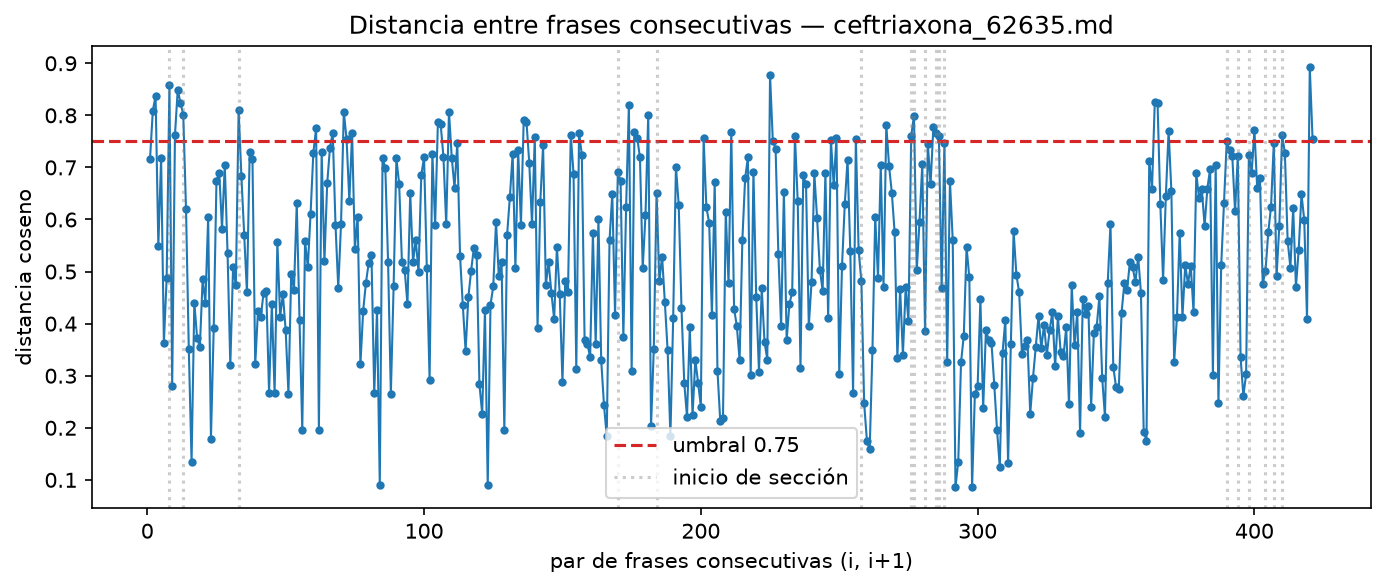
\includegraphics[keepaspectratio,alt={Distancia entre frases consecutivas de la ficha de ceftriaxona, con el umbral 0.75}]{exp_rag_chunking_distances.png}}
\end{center}

La gráfica no muestra picos aislados que separen temas: la distancia oscila entre 0.1 y 0.9
dentro de todas las secciones y los inicios de sección (líneas grises) no coinciden con los
picos. Las fichas técnicas cambian de tema de una frase a otra (listas de reacciones adversas,
tablas de dosis), así que el umbral no se puede elegir a ojo y lo elegimos con el barrido:

{\def\LTcaptype{none} % do not increment counter
\scriptsize\setlength{\tabcolsep}{1.5pt}
\begin{longtable}[]{@{}
  >{\raggedright\arraybackslash}p{(\linewidth - 14\tabcolsep) * \real{0.1250}}
  >{\raggedright\arraybackslash}p{(\linewidth - 14\tabcolsep) * \real{0.1250}}
  >{\raggedright\arraybackslash}p{(\linewidth - 14\tabcolsep) * \real{0.1250}}
  >{\raggedright\arraybackslash}p{(\linewidth - 14\tabcolsep) * \real{0.1250}}
  >{\raggedright\arraybackslash}p{(\linewidth - 14\tabcolsep) * \real{0.1250}}
  >{\raggedright\arraybackslash}p{(\linewidth - 14\tabcolsep) * \real{0.1250}}
  >{\raggedright\arraybackslash}p{(\linewidth - 14\tabcolsep) * \real{0.1250}}
  >{\raggedright\arraybackslash}p{(\linewidth - 14\tabcolsep) * \real{0.1250}}@{}}
\toprule\noalign{}
\begin{minipage}[b]{\linewidth}\raggedright
Umbral
\end{minipage} & \begin{minipage}[b]{\linewidth}\raggedright
Chunks
\end{minipage} & \begin{minipage}[b]{\linewidth}\raggedright
Media (car.)
\end{minipage} & \begin{minipage}[b]{\linewidth}\raggedright
Sin resolver
\end{minipage} & \begin{minipage}[b]{\linewidth}\raggedright
Cortes semánticos
\end{minipage} & \begin{minipage}[b]{\linewidth}\raggedright
Cortes por tamaño
\end{minipage} & \begin{minipage}[b]{\linewidth}\raggedright
Dense Recall@5 / MRR
\end{minipage} & \begin{minipage}[b]{\linewidth}\raggedright
Hybrid Recall@5 / MRR
\end{minipage} \\
\midrule\noalign{}
\endhead
\bottomrule\noalign{}
\endlastfoot
0.50 & 8272 & 198 & 16 & 7414 & 12 & 0.350 / 0.311 & 0.370 / 0.343 \\
0.60 & 5630 & 272 & 12 & 4731 & 53 & 0.433 / 0.428 & 0.447 / 0.458 \\
0.65 & 4388 & 338 & 10 & 3434 & 108 & 0.473 / 0.457 & 0.458 / 0.442 \\
0.70 & 3334 & 433 & 5 & 2258 & 230 & 0.548 / 0.535 & 0.548 / 0.513 \\
\textbf{0.75} & \textbf{2406} & \textbf{585} & \textbf{3} & \textbf{1171} & \textbf{389} & \textbf{0.543 / 0.567} & \textbf{0.568 / 0.592} \\
0.80 & 1825 & 758 & 2 & 444 & 535 & 0.578 / 0.569 & 0.588 / 0.591 \\
0.85 & 1563 & 879 & 1 & 102 & 615 & 0.643 / 0.617 & 0.653 / 0.632 \\
0.90 & 1496 & 916 & 1 & 12 & 638 & 0.653 / 0.607 & 0.653 / 0.628 \\
\end{longtable}
}

"Sin resolver" son las preguntas del gold cuya evidencia no está entera en ningún chunk. Como
referencia, el chunking recursivo (\texttt{chunk\_\allowbreak{}size=\allowbreak{}800}) da 2626 chunks de 556 caracteres de media:
800 es el tamaño máximo, y las secciones cortas y los finales de sección dan chunks menores.

\textbf{Qué concluimos.} Elegimos \textbf{0.75}, sabiendo que no es el umbral con mejores números: 0.85 y
0.9 tienen unos 0.06--0.09 más de Recall@5 (3--4 preguntas de 50) y algo más de MRR. No los
elegimos porque en ellos el criterio semántico casi no actúa: a partir de 0.8 los cortes por
tamaño superan a los semánticos, y en 0.85 y 0.9 quedan 102 y 12 cortes semánticos frente a más
de 600 por tamaño. Es decir, eso ya no es chunking semántico sino trocear cada sección cada 1500
caracteres, y la mejora se explica porque los chunks son más grandes: es más fácil que contengan
la evidencia entera (hay menos preguntas sin resolver) y hay menos chunks entre los que elegir.
Además, chunks de 900 caracteres meten más texto irrelevante en el prompt de generación. 0.75 es
el umbral más alto en el que el criterio semántico sigue haciendo la mayor parte de los cortes,
empata en MRR del híbrido con 0.8 y tiene una longitud media (585) parecida a la del recursivo
(556), lo que hace justa la comparación entre los dos chunkings. Con 50 preguntas, la diferencia
entre 0.75 y 0.8 (unas 2 preguntas) no es significativa.

\begin{center}\rule{0.5\linewidth}{0.5pt}\end{center}

\subsubsection{2026-10-29 · Fase 3 · Chunking recursivo frente a semántico, tres retrievers y barrido de λ}

\textbf{Qué queríamos saber.} Qué chunking y qué retriever recuperan mejor sobre el conjunto dorado,
y qué λ usar en el híbrido.

\textbf{Qué hicimos.} \texttt{rag/\allowbreak{}evaluate.py} trocea el corpus con las dos estrategias: recursivo
(\texttt{chunk\_\allowbreak{}size=\allowbreak{}800}, \texttt{overlap=\allowbreak{}100}) y semántico (umbral 0.75), ambos por secciones y con el
encabezado de la sección delante de cada chunk. Para cada una construye BM25, denso
(Qwen3-Embedding-0.6B con la instrucción por defecto) e híbrido. Como los ids de los chunks
cambian con la estrategia, los fragmentos relevantes de cada pregunta se calculan buscando la
evidencia del gold dentro del texto de los chunks. Con eso calcula Recall@5 y MRR de cada
retriever y repite el híbrido con λ de 0 a 1 en pasos de 0.1:

\begin{lstlisting}
uv run python -m rag.evaluate --gold rag/gold/gold.jsonl --k 5 --out reports/phase3_eval.json
\end{lstlisting}

\textbf{Qué pasó.} Todas las métricas son sobre las preguntas resueltas, las que tienen algún chunk
que contiene su evidencia: 48 en recursivo y 47 en semántico. Barrido de λ del híbrido (peso de BM25; λ = 0 es el denso solo y λ = 1 es BM25
solo), con el mejor λ de cada chunking en negrita:

{\def\LTcaptype{none} % do not increment counter
\scriptsize\setlength{\tabcolsep}{1pt}
\begin{longtable}[]{@{}
  >{\raggedright\arraybackslash}p{(\linewidth - 22\tabcolsep) * \real{0.2000}}
  >{\raggedright\arraybackslash}p{(\linewidth - 22\tabcolsep) * \real{0.0727}}
  >{\raggedright\arraybackslash}p{(\linewidth - 22\tabcolsep) * \real{0.0727}}
  >{\raggedright\arraybackslash}p{(\linewidth - 22\tabcolsep) * \real{0.0727}}
  >{\raggedright\arraybackslash}p{(\linewidth - 22\tabcolsep) * \real{0.0727}}
  >{\raggedright\arraybackslash}p{(\linewidth - 22\tabcolsep) * \real{0.0727}}
  >{\raggedright\arraybackslash}p{(\linewidth - 22\tabcolsep) * \real{0.0727}}
  >{\raggedright\arraybackslash}p{(\linewidth - 22\tabcolsep) * \real{0.0727}}
  >{\raggedright\arraybackslash}p{(\linewidth - 22\tabcolsep) * \real{0.0727}}
  >{\raggedright\arraybackslash}p{(\linewidth - 22\tabcolsep) * \real{0.0727}}
  >{\raggedright\arraybackslash}p{(\linewidth - 22\tabcolsep) * \real{0.0727}}
  >{\raggedright\arraybackslash}p{(\linewidth - 22\tabcolsep) * \real{0.0727}}@{}}
\toprule\noalign{}
\begin{minipage}[b]{\linewidth}\raggedright
λ
\end{minipage} & \begin{minipage}[b]{\linewidth}\raggedright
0.0
\end{minipage} & \begin{minipage}[b]{\linewidth}\raggedright
0.1
\end{minipage} & \begin{minipage}[b]{\linewidth}\raggedright
0.2
\end{minipage} & \begin{minipage}[b]{\linewidth}\raggedright
0.3
\end{minipage} & \begin{minipage}[b]{\linewidth}\raggedright
0.4
\end{minipage} & \begin{minipage}[b]{\linewidth}\raggedright
0.5
\end{minipage} & \begin{minipage}[b]{\linewidth}\raggedright
0.6
\end{minipage} & \begin{minipage}[b]{\linewidth}\raggedright
0.7
\end{minipage} & \begin{minipage}[b]{\linewidth}\raggedright
0.8
\end{minipage} & \begin{minipage}[b]{\linewidth}\raggedright
0.9
\end{minipage} & \begin{minipage}[b]{\linewidth}\raggedright
1.0
\end{minipage} \\
\midrule\noalign{}
\endhead
\bottomrule\noalign{}
\endlastfoot
Recursivo Recall@5 & 0.642 & 0.642 & 0.642 & 0.642 & \textbf{0.642} & 0.611 & 0.569 & 0.503 & 0.465 & 0.444 & 0.424 \\
Recursivo MRR & 0.568 & 0.577 & 0.593 & 0.612 & \textbf{0.632} & 0.616 & 0.502 & 0.481 & 0.445 & 0.413 & 0.394 \\
Semántico Recall@5 & 0.578 & 0.578 & 0.578 & \textbf{0.583} & 0.583 & 0.605 & 0.594 & 0.514 & 0.486 & 0.454 & 0.475 \\
Semántico MRR & 0.603 & 0.616 & 0.627 & \textbf{0.647} & 0.637 & 0.630 & 0.539 & 0.497 & 0.447 & 0.425 & 0.417 \\
\end{longtable}
}

Resultados de cada retriever, con el híbrido en λ = 0.5 y en el mejor λ:

{\def\LTcaptype{none} % do not increment counter
\scriptsize\setlength{\tabcolsep}{1.5pt}
\begin{longtable}[]{@{}
  >{\raggedright\arraybackslash}p{(\linewidth - 16\tabcolsep) * \real{0.1111}}
  >{\raggedright\arraybackslash}p{(\linewidth - 16\tabcolsep) * \real{0.1111}}
  >{\raggedright\arraybackslash}p{(\linewidth - 16\tabcolsep) * \real{0.1111}}
  >{\raggedright\arraybackslash}p{(\linewidth - 16\tabcolsep) * \real{0.1111}}
  >{\raggedright\arraybackslash}p{(\linewidth - 16\tabcolsep) * \real{0.1111}}
  >{\raggedright\arraybackslash}p{(\linewidth - 16\tabcolsep) * \real{0.1111}}
  >{\raggedright\arraybackslash}p{(\linewidth - 16\tabcolsep) * \real{0.1111}}
  >{\raggedright\arraybackslash}p{(\linewidth - 16\tabcolsep) * \real{0.1111}}
  >{\raggedright\arraybackslash}p{(\linewidth - 16\tabcolsep) * \real{0.1111}}@{}}
\toprule\noalign{}
\begin{minipage}[b]{\linewidth}\raggedright
Chunking
\end{minipage} & \begin{minipage}[b]{\linewidth}\raggedright
Chunks
\end{minipage} & \begin{minipage}[b]{\linewidth}\raggedright
Media
\end{minipage} & \begin{minipage}[b]{\linewidth}\raggedright
Sin resolver
\end{minipage} & \begin{minipage}[b]{\linewidth}\raggedright
BM25 Recall@5 / MRR
\end{minipage} & \begin{minipage}[b]{\linewidth}\raggedright
Dense Recall@5 / MRR
\end{minipage} & \begin{minipage}[b]{\linewidth}\raggedright
Hybrid λ=0.5 Recall@5 / MRR
\end{minipage} & \begin{minipage}[b]{\linewidth}\raggedright
Mejor λ
\end{minipage} & \begin{minipage}[b]{\linewidth}\raggedright
Hybrid mejor λ Recall@5 / MRR
\end{minipage} \\
\midrule\noalign{}
\endhead
\bottomrule\noalign{}
\endlastfoot
Recursivo & 2626 & 556 & 2 (14, 44) & 0.424 / 0.394 & 0.642 / 0.568 & 0.611 / 0.616 & 0.4 & \textbf{0.642 / 0.632} \\
Semántico 0.75 & 2406 & 585 & 3 (5, 7, 10) & 0.475 / 0.417 & 0.578 / 0.603 & 0.605 / 0.630 & 0.3 & 0.583 / \textbf{0.647} \\
\end{longtable}
}

En el barrido de λ se ven tres cosas:

\begin{itemize}
\tightlist
\item
  Entre λ = 0 y el mejor λ el Recall@5 apenas cambia (0.642 en recursivo, 0.578--0.583 en
  semántico), pero el MRR sube de 0.568 a 0.632 en recursivo (λ = 0.4) y de 0.603 a 0.647 en
  semántico (λ = 0.3). Es decir, añadir un poco de BM25 no mete chunks relevantes nuevos en el
  top 5, sino que sube de posición los que el denso ya encontraba.
\item
  A partir de λ = 0.6 las dos métricas caen rápido (en recursivo, el MRR baja a 0.502 con
  λ = 0.6): el ranking pasa a estar dominado por BM25.
\item
  BM25 solo (λ = 1) es la peor configuración en los dos chunkings: coincide con la columna de
  BM25 de la segunda tabla.
\end{itemize}

Las preguntas sin resolver no se pueden puntuar porque ningún chunk contiene entero ninguno de
sus fragmentos de evidencia. La salida de \texttt{rag/\allowbreak{}evaluate.py} las lista con la longitud de cada
fragmento:

{\def\LTcaptype{none} % do not increment counter
\small\setlength{\tabcolsep}{3pt}
\begin{longtable}[]{@{}lll@{}}
\toprule\noalign{}
Chunking & Pregunta & Fragmentos de evidencia (caracteres) \\
\midrule\noalign{}
\endhead
\bottomrule\noalign{}
\endlastfoot
Recursivo & 14 (tendinitis con levofloxacino) & 685 \\
Recursivo & 44 (sobredosis de morfina) & 683 y 161 \\
Semántico & 5 (contenido del vial de ceftriaxona) & 421 \\
Semántico & 7 (reconstitución de la amoxicilina) & 389 \\
Semántico & 10 (envases de enoxaparina) & 707 y 276 \\
\end{longtable}
}

Todos los fragmentos caben en el tamaño máximo de su chunking (800 y 1500 caracteres), así que
no quedan sin resolver por ser largos: un corte cae en mitad de la evidencia y la reparte entre
dos chunks. En recursivo es el divisor, que corta donde se le acaba el espacio. En semántico es
un corte semántico o por tamaño.

\textbf{Qué concluimos.} El denso gana a BM25 con diferencia. Creemos que se debe a las preguntas
coloquiales e inversas (de síntoma a fármaco) del gold (ver la entrada del conjunto dorado), que
no comparten palabras con la ficha. BM25 sirve como complemento con un
peso pequeño: nuestra hipótesis es que sube el chunk bueno por coincidencia exacta con el nombre
del fármaco o con cifras, en fichas de la misma familia que el denso confunde (cefalosporinas,
carbapenems) aunque no lo hemos verificado pregunta a pregunta. Los dos chunkings quedan prácticamente
empatados en MRR. Sin embargo, el recursivo tiene mejor recall y una pregunta menos sin resolver, así que
\textbf{\texttt{/\allowbreak{}rag} usa chunking recursivo e híbrido con λ = 0.4}. Elegimos λ por MRR porque el endpoint
devuelve pocos fragmentos y lo que importa es que el bueno salga primero. El análisis de las preguntas que
fallan, por categoría del gold, está en la entrada siguiente. La comparación de instrucciones
de embedding está en la entrada del 2026-11-01 (Instrucción de la consulta en los embeddings).

\begin{center}\rule{0.5\linewidth}{0.5pt}\end{center}

\subsubsection{2026-10-30 · Fase 3 · Preguntas que fallan, por categoría del gold}

\textbf{Qué queríamos saber.} En qué tipos de pregunta falla la recuperación y si se cumple la
hipótesis de la entrada anterior (que el denso gana por las preguntas coloquiales e inversas).

\textbf{Qué hicimos.} Añadimos a \texttt{rag/\allowbreak{}evaluate.py} las métricas por categoría del gold y la lista de
preguntas que fallan con el híbrido (con la ficha de la evidencia y la de cada fragmento
recuperado). Las categorías se asignan por el número de pregunta, en el orden del gold. Mismo
comando que en la entrada anterior.

\textbf{Qué pasó.} Híbrido con chunking recursivo y λ = 0.4 (Recall@5 / MRR y número de fallos):

{\def\LTcaptype{none} % do not increment counter
\small\setlength{\tabcolsep}{3pt}
\begin{longtable}[]{@{}llll@{}}
\toprule\noalign{}
Categoría & Preguntas & Recall@5 / MRR & Fallos \\
\midrule\noalign{}
\endhead
\bottomrule\noalign{}
\endlastfoot
Un medicamento, una sección & 15 & 0.571 / 0.524 & 6 \\
Un medicamento, varias secciones & 8 & 0.521 / 0.812 & 1 \\
Varios medicamentos & 8 & 0.583 / 0.463 & 2 \\
Inversas & 8 & 1.000 / 1.000 & 0 \\
Lenguaje coloquial & 5 & 0.250 / 0.250 & 3 \\
Premisa dudosa & 3 & 0.667 / 0.700 & 1 \\
Cálculo & 3 & 1.000 / 0.567 & 0 \\
\end{longtable}
}

En los 13 fallos, la ficha correcta está entre los cinco fragmentos recuperados: lo que falla
es la sección, no el fármaco.

\textbf{Qué concluimos.} Las inversas, que nos preocupaban, salen perfectas. Las peores son las
coloquiales: "¿cuánto me dura la vancomicina ya preparada?" lleva a la ficha de la vancomicina,
pero no a la sección de periodo de validez. La hipótesis se cumple solo en parte, porque en
recursivo el denso gana a BM25 en todas las categorías, no solo en esas dos. También vimos que
las preguntas 6 y 41 tienen evidencias tan genéricas que aparecen en varias fichas (3 y 7), y
habría que alargarlas. Con tan pocas preguntas por categoría, estos resultados son orientativos.

\begin{center}\rule{0.5\linewidth}{0.5pt}\end{center}

\subsubsection{\texorpdfstring{2026-10-29 · Fase 3 · Generación con citas: primera prueba de \texttt{/\allowbreak{}rag}}{2026-10-29 · Fase 3 · Generación con citas: primera prueba de /rag}}

\textbf{Qué queríamos saber.} Si \texttt{POST /\allowbreak{}rag} funciona de principio a fin con nuestro modelo de
razonamiento de la fase 1 como generador: si recupera, si cita fragmentos que existen y si dice
que no sabe cuando el corpus no tiene la respuesta.

\textbf{Qué hicimos.} \texttt{rag/\allowbreak{}generate.py} es lo que hay detrás de \texttt{POST /\allowbreak{}rag}. Al arrancar lee el corpus,
lo trocea con chunking recursivo, construye los tres retrievers (híbrido con λ = 0.4, según el
barrido de la entrada anterior) y carga el generador. El índice denso se guarda en \texttt{rag/\allowbreak{}index/\allowbreak{}}
para no reembeber el corpus en cada arranque. Para cada pregunta recupera los \texttt{top\_\allowbreak{}k} mejores
fragmentos y los mete en el prompt aumentado con su identificador. Después genera la respuesta y
extrae las citas, quedándose solo con las que existen entre los fragmentos devueltos.

El generador se toma de las mismas variables que \texttt{/\allowbreak{}reasoning}, \texttt{ARCA\_\allowbreak{}RLM\_\allowbreak{}BASE\_\allowbreak{}MODEL} y
\texttt{ARCA\_\allowbreak{}RLM\_\allowbreak{}ADAPTER} del \texttt{.env}: nuestro modelo de la fase 1, Qwen3-0.6B con el adaptador LoRA
\texttt{rlm/\allowbreak{}weights/\allowbreak{}final\_\allowbreak{}rlm\_\allowbreak{}lora\_\allowbreak{}sin\_\allowbreak{}kl}. Como se entrenó con el prompt de sistema de R1-Zero, el
prompt aumentado se mete en ese prompt de sistema; el modelo razona en \texttt{\textless{}think\textgreater{}} y la respuesta
es el bloque \texttt{\textless{}answer\textgreater{}}, igual que en \texttt{/\allowbreak{}reasoning}. La decodificación es voraz.

Levantamos la API desde la raíz del repositorio y comprobamos que la fase \texttt{rag} aparece como
\texttt{ready}:

\begin{lstlisting}
uv run uvicorn api.app:app --port 8001
curl localhost:8001/health
\end{lstlisting}

Hicimos tres peticiones, una con cada retriever. Las peticiones
aparecen con curl pero también las hicimos exponiendo la api con ngrok usando Postman
confirmando que funciona.

\textbf{Qué pasó.}

\textbf{Caso 1.} Una pregunta del gold, con el híbrido:

\begin{lstlisting}
curl -s -X POST localhost:8001/rag -H 'Content-Type: application/json' \
  -d '{"question": "¿Cómo debe ajustarse la dosis de cefotaxima en pacientes con insuficiencia renal grave?", "top_k": 5, "retriever": "hybrid"}'
\end{lstlisting}

Fragmentos recuperados: ceftriaxona 4.2 (0.91), cefotaxima 4.4 (0.84, \texttt{7f4d67e570-0026}),
ceftazidima 4.2 (0.49, \texttt{910ed8f16d-0011}), cefuroxima 4.2.1 (0.45) y cefazolina 4.2 (0.44).
Citas: ninguna. Respuesta:

\begin{quote}
La dosis de cefotaxima debe ajustarse según el cálculo del aclaramiento de creatinina, que se
basa en el valor de la creatinina sérica. La dosis de carga inicial es de 1 g y las dosis de
mantenimiento se basan en el aclaramiento de creatinina. La vigilancia clínica de la seguridad
y la eficacia debe incluir la monitorización de la función renal.
\end{quote}

El único fragmento de cefotaxima es el de la sección 4.4, no el de la 4.2 que tiene la respuesta
(\texttt{7f4d67e570-0011}), así que no da la regla concreta de la ficha (reducir a la mitad la dosis de
mantenimiento si el aclaramiento es \textless{} 10 ml/min). Además, "la dosis de carga inicial es de 1 g"
es la dosis de la \textbf{ceftazidima} (\texttt{910ed8f16d-0011}), atribuida a la cefotaxima.

\textbf{Caso 2.} Una pregunta coloquial, con el denso:

\begin{lstlisting}
curl -s -X POST localhost:8001/rag -H 'Content-Type: application/json' \
  -d '{"question": "¿Se puede dar meropenem con probenecid?", "top_k": 5, "retriever": "dense"}'
\end{lstlisting}

Fragmentos recuperados: meropenem 4.5 (0.86, \texttt{de9b07db3c-0021}), meropenem 4.4 (0.76),
amoxicilina 4.5 (0.71), meropenem 4.4 (0.68) y meropenem 4.4 (0.68). Citas: ninguna. Respuesta:

\begin{quote}
Se puede administrar meropenem con probenecid, pero se debe considerar la inhibición de la
excreción renal de meropenem por probenecid. La combinación puede afectar la dosis y la
eficacia, por lo que se recomienda consultar a un médico antes de administrar ambas medicamentos.
\end{quote}

El primer fragmento tiene la respuesta: el probenecid inhibe la excreción renal del meropenem y
"se requiere precaución". El modelo recoge la interacción, pero la conclusión ("ajustar la dosis
de probenecid") no está en ningún fragmento.

\textbf{Caso 3.} Una pregunta que el corpus no puede responder (el omeprazol no está en el corpus),
con BM25:

\begin{lstlisting}
curl -s -X POST localhost:8001/rag -H 'Content-Type: application/json' \
  -d '{"question": "¿Cuál es la dosis de omeprazol intravenoso en una hemorragia digestiva?", "top_k": 5, "retriever": "bm25"}'
\end{lstlisting}

Fragmentos recuperados: enoxaparina 4.4 (17.9), heparina 4.9 (17.0), furosemida 4.2 (16.9),
furosemida 4.2 (16.3) y azitromicina 4.2.2 (15.9). Citas: ninguna. Respuesta:

\begin{quote}
La información proporcionada no incluye datos sobre la dosis de omeprazol intravenosa en casos
de hemorragia digestiva. No hay referencias o datos sobre este medicamento en la información disponible.
\end{quote}

BM25 empareja palabras como "dosis", "intravenoso" o "hemorragia" y trae fragmentos sin relación,
pero el modelo reconoce que no tiene la información. Es el comportamiento esperado.

\textbf{Qué concluimos.} La API funciona con los tres retrievers, y la recuperación y el prompt
aumentado son los esperados. Con nuestro modelo como generador, en cambio, las respuestas no
cumplen lo que se pide en \texttt{/\allowbreak{}rag}. No cita ningún fragmento, aunque el prompt lo pide. Mezcla
datos de fármacos distintos (la dosis de la ceftazidima) y añade conclusiones que no están en
los fragmentos (ajustar la dosis de probenecid). Lo único que hace bien es reconocer que el
omeprazol no está. Creemos que se debe al modelo y no al pipeline. El adaptador se entrenó para
calcular dosis a partir de un enunciado corto y responder con un número en \texttt{\textless{}answer\textgreater{}}, no para
leer varios fragmentos largos y citar su origen, y un modelo de 0.6B tiene poca capacidad para
separar cinco fichas parecidas en el mismo contexto. Habría que entrenar al modelo para que
aprendiera a citar.

\begin{center}\rule{0.5\linewidth}{0.5pt}\end{center}

\subsubsection{2026-11-01 · Fase 3 · ¿Sabe citar el generador? Comparación de cuatro modelos}

\textbf{Qué queríamos saber.} En la primera prueba de \texttt{/\allowbreak{}rag} nuestro modelo (Qwen3-0.6B con el adaptador
de la fase 1) no citaba ningún fragmento. Queremos saber si es culpa del entrenamiento (SFT y GRPO
nos habrían quitado la capacidad de citar) o del tamaño: ¿cita el 0.6B base sin adaptador?, ¿y
uno mayor? Si el base cita y el nuestro no, hay que arreglar el entrenamiento; si no cita ni el
base, habría que enseñarle a citar o cambiar de modelo.

\textbf{Qué hicimos.} Misma recuperación y mismo prompt para los cuatro: chunking recursivo, híbrido
con λ = 0.4, \texttt{top\_\allowbreak{}k =\allowbreak{} 5}. Solo cambia el generador, que se elige con las variables de \texttt{/\allowbreak{}rag}.
\texttt{rag/\allowbreak{}compare\_\allowbreak{}generators.py} genera la respuesta de cada pregunta del gold que tiene fragmento
relevante (48 de 50; dos no se resuelven con el chunking recursivo) y de 8 preguntas que el
corpus no puede responder (omeprazol, metformina, atorvastatina, warfarina, diazepam rectal,
precio de la vancomicina, descubridor de la penicilina, insulina glargina). Decodificación
greedy, 1024 tokens máximo; los modelos base van sin razonamiento (\texttt{enable\_\allowbreak{}thinking=\allowbreak{}False}) y el
adaptador con el prompt de sistema R1-Zero de la fase 1.

\begin{lstlisting}
ARCA_RLM_BASE_MODEL=Qwen/Qwen3-0.6B uv run python -m rag.compare_generators --tag qwen3-0.6b-base
ARCA_RLM_BASE_MODEL=Qwen/Qwen3-0.6B ARCA_RLM_ADAPTER=rlm/weights/final_rlm_lora_sin_kl \
  uv run python -m rag.compare_generators --tag qwen3-0.6b-rlm
ARCA_RLM_BASE_MODEL=Qwen/Qwen3-1.7B uv run python -m rag.compare_generators --tag qwen3-1.7b
ARCA_RLM_BASE_MODEL=Qwen/Qwen3-4B   uv run python -m rag.compare_generators --tag qwen3-4b
\end{lstlisting}

Las respuestas completas están en \texttt{reports/\allowbreak{}rag/\allowbreak{}generators/\allowbreak{}\textless{}tag\textgreater{}.json}. El script no carga el
\texttt{.env}, así que el adaptador solo se aplica donde se indica (el campo \texttt{model} de cada JSON lo
confirma). Una respuesta "cita" si contiene algún id entre corchetes que existe entre los cinco
fragmentos devueltos. El reparto de las respuestas sin cita usa un detector de abstención por
expresiones regulares, que es orientativo.

\textbf{Qué pasó.} En 35 de las 48 preguntas el fragmento correcto estaba entre los cinco recuperados,
igual para los cuatro modelos.

{\def\LTcaptype{none} % do not increment counter
\scriptsize\setlength{\tabcolsep}{1.5pt}
\begin{longtable}[]{@{}
  >{\raggedright\arraybackslash}p{(\linewidth - 14\tabcolsep) * \real{0.1250}}
  >{\raggedright\arraybackslash}p{(\linewidth - 14\tabcolsep) * \real{0.1250}}
  >{\raggedright\arraybackslash}p{(\linewidth - 14\tabcolsep) * \real{0.1250}}
  >{\raggedright\arraybackslash}p{(\linewidth - 14\tabcolsep) * \real{0.1250}}
  >{\raggedright\arraybackslash}p{(\linewidth - 14\tabcolsep) * \real{0.1250}}
  >{\raggedright\arraybackslash}p{(\linewidth - 14\tabcolsep) * \real{0.1250}}
  >{\raggedright\arraybackslash}p{(\linewidth - 14\tabcolsep) * \real{0.1250}}
  >{\raggedright\arraybackslash}p{(\linewidth - 14\tabcolsep) * \real{0.1250}}@{}}
\toprule\noalign{}
\begin{minipage}[b]{\linewidth}\raggedright
Modelo
\end{minipage} & \begin{minipage}[b]{\linewidth}\raggedright
Cita algo
\end{minipage} & \begin{minipage}[b]{\linewidth}\raggedright
Cita el fragmento correcto
\end{minipage} & \begin{minipage}[b]{\linewidth}\raggedright
Sin cita: abstención
\end{minipage} & \begin{minipage}[b]{\linewidth}\raggedright
Sin cita: fragmento correcto no recuperado
\end{minipage} & \begin{minipage}[b]{\linewidth}\raggedright
Sin cita: fragmento correcto recuperado
\end{minipage} & \begin{minipage}[b]{\linewidth}\raggedright
Ids inventados
\end{minipage} & \begin{minipage}[b]{\linewidth}\raggedright
Preguntas sin respuesta que citan
\end{minipage} \\
\midrule\noalign{}
\endhead
\bottomrule\noalign{}
\endlastfoot
Qwen3-0.6B base & 17/48 (35 \%) & 14 & 12 & 4 & 15 & 0 & 0/8 \\
Qwen3-0.6B + adaptador (el nuestro), 1024 tokens & 6/48 (12,5 \%) & 5 & 9 & 6 & 18 & 0 & 0/6 \\
Qwen3-0.6B + adaptador (el nuestro), 1536 tokens & 5/48 (10,4 \%) & 3 & 8 & 8 & 22 & 0 & 0/8 \\
Qwen3-1.7B base & 38/48 (79 \%) & 26 & 6 & 1 & 3 & 0 & 3/8 \\
Qwen3-4B base & 45/48 (94 \%) & 33 & 3 & 0 & 0 & 0 & 2/8 \\
\end{longtable}
}

\emph{Fila del adaptador corregida (ver la entrada "Las citas eran ids del razonamiento"): 9 de las 48
respuestas con fragmento y 2 de las 8 sin respuesta se truncaron dentro del razonamiento (1024
tokens) y no cuentan como respuesta, por eso las 33 sin cita no suman 42 y las preguntas sin
respuesta son 6. Antes de corregirlo la tabla decía 14/48 (29 \%), 10, 9, 6, 19 y 1/8.}

Cuando el fragmento correcto está entre los recuperados, el modelo lo cita en 14 de 35 casos
(0.6B base), 5 y 3 (0.6B con adaptador, con 1024 y 1536 tokens), 26 (1.7B) y 33 (4B).

Lo que se ve al leer las respuestas:

\begin{itemize}
\tightlist
\item
  \textbf{0.6B base.} Cita poco y mal. Cuando cita, a veces copia la cabecera del contexto
  (\texttt{{[}id{]} (from fichero.md)}) en vez de citar al final de la afirmación. Mezcla fármacos (habla de
  abrocitinib y fluconazol en una pregunta de meropenem), inventa cifras (dexketoprofeno a
  "1,4 microgramos/kg/h") y se abstiene en inglés.
\item
  \textbf{0.6B con adaptador.} Peor que el base. En 9 de 48 respuestas el razonamiento se corta a los
  1024 tokens sin llegar a la respuesta, y esas respuestas devolvían el razonamiento como si fuera
  la respuesta, con sus ids contados como citas (ver la entrada siguiente a esta). Dice que la información no incluye "quién descubrió la penicilina" y a continuación
  responde "Alexander Fleming en 1928" con conocimiento propio.
\item
  \textbf{1.7B.} Cita en cuatro de cada cinco respuestas. Las sin cita son abstenciones o preguntas donde
  el fragmento correcto no se recuperó; solo 3 no citan teniendo el fragmento. En atorvastatina y
  warfarina, que el corpus no responde, cita un fragmento lateral y contesta con conocimiento propio.
\item
  \textbf{4B.} Cita en 45 de 48 y casi siempre el fragmento correcto cuando lo tiene. Las tres sin cita
  son abstenciones. En 6 de las 8 preguntas sin respuesta no cita nada y dice que la información no
  está. En warfarina cita fragmentos y explica el INR, y en
  diazepam rectal dice que no hay dosis pediátrica pero cita un fragmento relacionado.
\end{itemize}

Ningún modelo inventa ids. La comprobación de que los ids existen siempre se cumple, pero
\textbf{no garantiza que la afirmación esté en el fragmento citado}: el 1.7B y el 4B citan en preguntas
que el corpus no responde y el 0.6B con adaptador responde fuera del corpus. Citar es necesario y
no basta.

\textbf{Qué concluimos.}

\begin{enumerate}
\tightlist
\item
  \textbf{El 0.6B base ya citaba poco (35 \%), y con el adaptador cita bastante menos (10-12 \%).}
  Nuestra primera lectura, que el SFT y el GRPO no habían empeorado la capacidad de citar, se
  apoyaba en una cifra inflada: el 29 \% incluía ids mencionados mientras razonaba. Con la cifra
  corregida el adaptador queda por debajo del base, y la caída no se explica solo porque el
  razonamiento se trunque: con 1536 tokens terminan 43 de 48 respuestas y solo 5 citan (12 \%)
  frente al 35 \% del base (ver la entrada siguiente). Es una diferencia sobre 48 preguntas y
  una ejecución, así que la damos como indicio y no como medida.
\item
  \textbf{El factor determinante es el tamaño.} Con el mismo prompt, citar pasa de 35 \% (0.6B) a 79 \%
  (1.7B) y 94 \% (4B). El 0.6B no es capaz de seguir "cita los pasajes que uses" aunque el
  fragmento esté delante (15 casos sin cita con el fragmento recuperado), mientras que el 4B
  falla en 0.
\item
  \textbf{Hay que cambiar el generador de \texttt{/\allowbreak{}rag}, no entrenar al 0.6B.} Qwen3-4B es el que cumple lo
  que pide el README: cita, las citas existen y casi siempre apoyan la respuesta. Por lo tanto, para que el modelo cite correctamente deberíamos hacer SFT sobre un modelo que ya sepa citar, uno más grande que el de 0.6B. Para ello, habría que volver a hacer la fase 1 con un modelo más grande como el 4B. Para cambiarlo en las pruebas solo hay que poner
  \texttt{ARCA\_\allowbreak{}RLM\_\allowbreak{}BASE\_\allowbreak{}MODEL=\allowbreak{}Qwen/\allowbreak{}Qwen3-4B} y dejar \texttt{ARCA\_\allowbreak{}RLM\_\allowbreak{}ADAPTER} vacío.
\item
  \textbf{Parte de las respuestas sin cita no son culpa del generador.} Con los modelos grandes lo que
  queda sin citar es sobre todo abstención o fragmento no recuperado. Los fallos de recuperación
  se concentran en conservación, periodo de validez y envases, donde el texto del fragmento no
  contiene el nombre del fármaco (\texttt{6.3 Periodo de validez \textbar{} Antes de la apertura: 3 años…} es
  casi igual en las 47 fichas). Habría que ver si poniendo el
  nombre del fármaco en la cabecera del chunk, reembebiendo y repitiendo \texttt{rag.evaluate} los resultados mejoran.
\end{enumerate}

\begin{center}\rule{0.5\linewidth}{0.5pt}\end{center}

\subsubsection{2026-11-01 · Fase 3 · Instrucción de la consulta en los embeddings}

\textbf{Qué queríamos saber.} Qwen3-Embedding se entrena con una instrucción de tarea delante de la
consulta (\texttt{Instruct: ...\textbackslash{}nQuery: ...}) y los pasajes se embeben sin ella. Hasta ahora usábamos la
instrucción por defecto de \texttt{rag/\allowbreak{}embed.py}. Queremos saber cuánto cambia la recuperación si la
cambiamos, si una instrucción adaptada a nuestro dominio (fichas técnicas, enfermería) la mejora
y qué pasa sin instrucción o con una que no tiene que ver con la tarea.

\textbf{Qué hicimos.} \texttt{instruction\_\allowbreak{}sweep} en \texttt{rag/\allowbreak{}evaluate.py}. Los vectores de los pasajes no dependen
de la instrucción, así que se carga el índice denso persistido y solo cambia \texttt{query\_\allowbreak{}instruction}
(sin reembeber el corpus). Chunking recursivo, λ = 0.4 para el híbrido, k = 5 y las 48 preguntas
del gold con fragmento resuelto. Se compararon seis instrucciones (\texttt{QUERY\_\allowbreak{}INSTRUCTIONS}):
\texttt{default}; \texttt{none} (la consulta sin el prefijo \texttt{Instruct:}); \texttt{domain\_\allowbreak{}en} y \texttt{domain\_\allowbreak{}es}
(fragmento de la ficha técnica que responde a una pregunta de enfermería, en inglés y en español);
\texttt{drug\_\allowbreak{}first} (identificar primero el fármaco y recuperar la sección de su ficha) y \texttt{unrelated}
("Classify the sentiment of the following text."), un control que no tiene que ver con recuperar.

\begin{lstlisting}
uv run python -m rag.evaluate --gold rag/gold/gold.jsonl --k 5 --lam 0.4 --instruction-sweep
\end{lstlisting}

Resultados completos en \texttt{reports/\allowbreak{}phase3\_\allowbreak{}instruction\_\allowbreak{}sweep.json}. "Gana/pierde" son los números de
pregunta (desde 1) que el denso acierta/falla respecto a \texttt{default}.

\textbf{Qué pasó.}

{\def\LTcaptype{none} % do not increment counter
\scriptsize\setlength{\tabcolsep}{1.5pt}
\begin{longtable}[]{@{}
  >{\raggedright\arraybackslash}p{(\linewidth - 14\tabcolsep) * \real{0.1250}}
  >{\raggedright\arraybackslash}p{(\linewidth - 14\tabcolsep) * \real{0.1250}}
  >{\raggedright\arraybackslash}p{(\linewidth - 14\tabcolsep) * \real{0.1250}}
  >{\raggedright\arraybackslash}p{(\linewidth - 14\tabcolsep) * \real{0.1250}}
  >{\raggedright\arraybackslash}p{(\linewidth - 14\tabcolsep) * \real{0.1250}}
  >{\raggedright\arraybackslash}p{(\linewidth - 14\tabcolsep) * \real{0.1250}}
  >{\raggedright\arraybackslash}p{(\linewidth - 14\tabcolsep) * \real{0.1250}}
  >{\raggedright\arraybackslash}p{(\linewidth - 14\tabcolsep) * \real{0.1250}}@{}}
\toprule\noalign{}
\begin{minipage}[b]{\linewidth}\raggedright
Instrucción
\end{minipage} & \begin{minipage}[b]{\linewidth}\raggedright
Denso Recall@5
\end{minipage} & \begin{minipage}[b]{\linewidth}\raggedright
Denso MRR
\end{minipage} & \begin{minipage}[b]{\linewidth}\raggedright
Fallos (denso)
\end{minipage} & \begin{minipage}[b]{\linewidth}\raggedright
Híbrido Recall@5
\end{minipage} & \begin{minipage}[b]{\linewidth}\raggedright
Híbrido MRR
\end{minipage} & \begin{minipage}[b]{\linewidth}\raggedright
Gana
\end{minipage} & \begin{minipage}[b]{\linewidth}\raggedright
Pierde
\end{minipage} \\
\midrule\noalign{}
\endhead
\bottomrule\noalign{}
\endlastfoot
default & 0.642 & 0.568 & 13 & 0.642 & 0.632 & & \\
none & 0.653 & 0.605 & 12 & 0.663 & 0.652 & 3, 30 & 46 \\
domain\_\allowbreak{}en & 0.580 & 0.523 & 16 & 0.611 & 0.593 & 30 & 24, 31, 46, 49 \\
domain\_\allowbreak{}es & 0.590 & 0.553 & 16 & 0.622 & 0.622 & 30 & 21, 31, 46, 49 \\
drug\_\allowbreak{}first & 0.569 & 0.551 & 17 & 0.622 & 0.601 & & 24, 31, 46, 49 \\
unrelated & 0.000 & 0.000 & 48 & 0.000 & 0.000 & & 35 preguntas \\
\end{longtable}
}

\begin{itemize}
\tightlist
\item
  \textbf{Quitar la instrucción cambia poco.} \texttt{default} y \texttt{none} quedan dentro de un punto de Recall@5
  (0.642 y 0.653 en denso): una pregunta de diferencia sobre 48.
\item
  \textbf{Las instrucciones de dominio empeoran, no mejoran.} \texttt{domain\_\allowbreak{}en}, \texttt{domain\_\allowbreak{}es} y \texttt{drug\_\allowbreak{}first}
  bajan el denso 5-7 puntos (de 13 a 16-17 fallos) y las tres pierden las preguntas 31, 46 y 49
  (más la 24, o la 21 en \texttt{domain\_\allowbreak{}es}); en el híbrido bajan 2-3 puntos. Esperábamos lo contrario.
\item
  \textbf{El control hunde la recuperación.} Con la instrucción de sentimiento, los fragmentos mejor
  puntuados de una consulta tienen todos la misma similitud (0.547 en el caso que miramos), es
  decir, el vector de la consulta deja de depender de la pregunta y el ranking es casi constante.
  El híbrido también cae a 0. Creemos que es porque, con las puntuaciones del denso empatadas, el
  reescalado a {[}0, 1{]} da 1 a los 20 fragmentos del denso y BM25 no consigue sacar a ninguno de los
  suyos por encima; no lo hemos comprobado.
\end{itemize}

\textbf{Qué concluimos.}

\begin{enumerate}
\tightlist
\item
  \textbf{La instrucción importa, pero quitarla apenas cambia el resultado.} La diferencia entre
  \texttt{default} y \texttt{none} es de una pregunta y no la interpretamos con 48 preguntas y una sola
  ejecución. Lo que sí es claro es el efecto del control, que confirma que la instrucción
  participa de verdad en el vector de la consulta.
\item
  \textbf{Nuestra hipótesis de que una instrucción de dominio ayudaría no se cumple.} Las tres que
  mencionan fichas técnicas o el fármaco pierden las preguntas 31, 46 y 49. La 31 (y la 24 y la
  21 en alguna de ellas) son de "varios medicamentos", con dos fármacos en la consulta; la 46 es
  de premisa dudosa (amikacina y embarazo) y la 49 de cálculo. Nuestra explicación tentativa es que una instrucción que pide "el fragmento de
  la ficha" o "identificar el fármaco" empuja la consulta hacia un solo fármaco o hacia el estilo de
  ficha y se pierde el segundo. No lo hemos comprobado mirando los fragmentos recuperados.
\item
  \textbf{No cambiamos la instrucción de \texttt{/\allowbreak{}rag}.} \texttt{none} sale unas décimas por encima, pero la mejora
  no se distingue de una pregunta más. Dejamos la de por defecto, la que viene en \texttt{rag/\allowbreak{}embed.py}.
\end{enumerate}

\begin{center}\rule{0.5\linewidth}{0.5pt}\end{center}

\subsubsection{2026-11-02 · Fase 3 · Las citas del RLM eran ids que mencionaba mientras razonaba}

\textbf{Qué queríamos saber.} La tabla de la entrada anterior daba al RLM un 29 \% de respuestas con
cita, pero al leer sus respuestas varias empezaban por \texttt{\textless{}think\textgreater{} Vale, voy a resolverlo paso a paso…}. Queríamos saber de dónde salían esas citas y si eran citas de la respuesta o no.

\textbf{Qué vimos.} Las respuestas del RLM con \texttt{\textless{}think\textgreater{}} en el texto son 11 de las 56 generadas (9 de
las 48 con fragmento y 2 de las 8 sin respuesta). Todas miden entre 1021 y 1024 tokens, mientras que
el resto no pasa de 328. \texttt{MAX\_\allowbreak{}NEW\_\allowbreak{}TOKENS} era 1024: el modelo se quedaba sin tokens \textbf{antes de cerrar
el razonamiento}, sin \texttt{\textless{}/\allowbreak{}think\textgreater{}} ni \texttt{\textless{}answer\textgreater{}}. Entonces \texttt{split\_\allowbreak{}thinking} (\texttt{rlm/\allowbreak{}inference.py}) no
encuentra un bloque de razonamiento completo y, por diseño, devuelve todo el texto como respuesta. El
razonamiento truncado acababa siendo la respuesta de \texttt{/\allowbreak{}rag}, y \texttt{extract\_\allowbreak{}citations} contaba como
citas los ids que el modelo mencionaba al razonar ("\ldots el parágrafo {[}dd4c9e923a-0010{]}, que dice\ldots"). De
esas 11, 9 tenían citas. No era un fallo de \texttt{split\_\allowbreak{}thinking}: es un caso que el código no
distinguía de una respuesta normal.

Una cita tiene que salir de la respuesta, no del razonamiento. Con las respuestas truncadas tratadas
como "sin respuesta", el RLM cita en 6 de 48 preguntas (12,5 \%) y no en 14 (29 \%), y cita el
fragmento correcto en 5 y no en 10. Lo recalculamos sobre las respuestas ya guardadas, sin generar de
nuevo, y corregimos la fila del RLM en la entrada anterior.

\textbf{Qué hicimos.} Cuatro cambios, los tres primeros en \texttt{rag/\allowbreak{}generate.py}:

\begin{enumerate}
\tightlist
\item
  \texttt{final\_\allowbreak{}answer(raw)}: si la generación tiene \texttt{\textless{}think\textgreater{}} pero no \texttt{\textless{}/\allowbreak{}think\textgreater{}}, se cortó razonando y no
  hay respuesta; devuelve \texttt{TRUNCATED\_\allowbreak{}ANSWER} ("No se pudo completar la respuesta: el razonamiento
  del modelo se truncó.") en vez de una cadena vacía, para que se vea que falló. En el resto de
  casos usa \texttt{split\_\allowbreak{}thinking} como antes. Solo se aplica con adaptador.
\item
  \texttt{MAX\_\allowbreak{}NEW\_\allowbreak{}TOKENS} de 1024 a 1536 (un 50 \% más), para que al RLM le dé tiempo a cerrar el
  razonamiento.
\item
  \texttt{check\_\allowbreak{}citations(answer, valid\_\allowbreak{}ids)} separa los ids entre corchetes en válidos e inválidos
  (los que no están entre los fragmentos devueltos, ya sean ids inventados u otro texto entre
  corchetes como \texttt{{[}1{]}}). \texttt{extract\_\allowbreak{}citations} pasa a usarla, con la misma firma y resultado.
\item
  \texttt{RagResponse} en \texttt{api/\allowbreak{}schemas.py} gana el campo opcional \texttt{invalid\_\allowbreak{}citations: list{[}str{]}}
  (vacío por defecto, no cambia lo que la API devolvía) y \texttt{to\_\allowbreak{}response} lo rellena, además de
  escribir un aviso en el log cuando hay inválidos. Hasta ahora un id inventado se descartaba sin
  dejar rastro.
\end{enumerate}

\textbf{Qué pasó con 1536 tokens.} Repetimos solo el RLM con el cambio
(\texttt{reports/\allowbreak{}rag/\allowbreak{}generators/\allowbreak{}qwen3-0.6b-rlm-1536.json}):

{\def\LTcaptype{none} % do not increment counter
\footnotesize\setlength{\tabcolsep}{3pt}
\begin{longtable}[]{@{}
  >{\raggedright\arraybackslash}p{(\linewidth - 8\tabcolsep) * \real{0.2000}}
  >{\raggedright\arraybackslash}p{(\linewidth - 8\tabcolsep) * \real{0.2000}}
  >{\raggedright\arraybackslash}p{(\linewidth - 8\tabcolsep) * \real{0.2000}}
  >{\raggedright\arraybackslash}p{(\linewidth - 8\tabcolsep) * \real{0.2000}}
  >{\raggedright\arraybackslash}p{(\linewidth - 8\tabcolsep) * \real{0.2000}}@{}}
\toprule\noalign{}
\begin{minipage}[b]{\linewidth}\raggedright
RLM
\end{minipage} & \begin{minipage}[b]{\linewidth}\raggedright
Truncadas
\end{minipage} & \begin{minipage}[b]{\linewidth}\raggedright
Cita algo
\end{minipage} & \begin{minipage}[b]{\linewidth}\raggedright
Cita el fragmento correcto
\end{minipage} & \begin{minipage}[b]{\linewidth}\raggedright
Sin cita entre las que terminan
\end{minipage} \\
\midrule\noalign{}
\endhead
\bottomrule\noalign{}
\endlastfoot
1024 tokens (recalculado) & 9 de 48 (y 2 de 8 sin respuesta) & 6/48 (12,5 \%) & 5 & 33 de 39 \\
1536 tokens & 5 de 48 (y 0 de 8 sin respuesta) & 5/48 (10,4 \%) & 3 & 38 de 43 \\
\end{longtable}
}

Seis de las nueve respuestas truncadas con 1024 tokens terminan ahora (tres de ellas citan), pero
dos de las que terminaban pasan a truncarse, de ahí 9 → 5. Y el total de citas, que parece estable
(6 frente a 5), esconde mucho cambio: de las 6 preguntas que citaban con 1024 tokens, solo 2
vuelven a citar. De las 39 respuestas que ya terminaban con 1024 tokens, 33 tienen un texto
distinto al repetir, aunque la decodificación sea greedy (6 salen idénticas). La generación del RLM
no es reproducible entre ejecuciones, algo que ya vimos al llamar dos veces a la API con la misma
pregunta, y no hemos investigado la causa. Ya no queda ningún \texttt{\textless{}think\textgreater{}} suelto en las respuestas.
Los ids inventados siguen siendo 0 y ninguna de las 8 preguntas sin respuesta cita.

Comprobamos que la API sigue funcionando: los tests pasan, los tres retrievers de
\texttt{POST /\allowbreak{}rag} responden con el campo nuevo y un retriever inválido sigue dando 422. Los resultados de
recuperación no cambian (\texttt{reports/\allowbreak{}phase3\_\allowbreak{}eval.json}, el barrido del umbral y el de instrucciones
salen idénticos) y los tres modelos sin adaptador no se ven afectados: sus respuestas más largas son
de 296, 686 y 750 tokens, por debajo del límite antiguo.

\textbf{Qué concluimos.}

\begin{enumerate}
\tightlist
\item
  \textbf{La cifra de citas del RLM estaba inflada.} Más de la mitad de las citas que contaba (8 de las 14
  respuestas con cita eran de respuestas truncadas) venían del razonamiento. Con el límite de 1024
  tokens el RLM cita en el 12,5 \% de las preguntas, frente al 35 \% del 0.6B base.
\item
  \textbf{Cambia una conclusión de la entrada anterior.} Allí decíamos que el SFT y el GRPO no nos habían
  quitado la capacidad de citar. Con la cifra corregida el adaptador cita menos que el base, y la
  ejecución con 1536 tokens indica que no es solo el truncamiento: con casi todas las respuestas
  terminadas (43 de 48) cita el 12 \%, frente al 35 \% del base. Lo más probable es que el adaptador,
  entrenado para devolver un número en \texttt{\textless{}answer\textgreater{}}, haya perdido parte de la tendencia a citar; no
  lo hemos aislado (haría falta el mismo prompt con el adaptador desactivado y la misma plantilla
  de razonamiento, y más preguntas).
\item
  \textbf{Un id entre corchetes no es una cita.} La comprobación automática que ya había (el id existe
  entre los fragmentos devueltos) no distingue dónde lo escribió el modelo. Ahora solo se mira el
  texto de la respuesta, pero seguimos sin comprobar que la afirmación esté en el fragmento
  citado; para eso haría falta un modelo juez.
\end{enumerate}

\textbf{Limitaciones.} Como la generación no es reproducible, las cifras de citas de cualquiera de los
cuatro modelos (no solo el RLM) llevan un ruido que no hemos medido; no hemos repetido ninguna
ejecución varias veces. El recálculo con 1024 tokens usa las respuestas ya guardadas y trata las truncadas
como "sin respuesta", sin volver a generar. El detector de abstención sigue siendo una expresión
regular. 48 preguntas y una sola ejecución.

\begin{center}\rule{0.5\linewidth}{0.5pt}\end{center}

\subsubsection{2026-11-03 · Fase 4 · Timeout por herramienta del agente}

\textbf{Qué queríamos saber.} El README de la fase 4 pide un "límite de tiempo por herramienta" en el
bucle ReAct. Lo implementamos primero con 60 s, una estimación sin datos. Queríamos un valor
elegido con lo que tardan de verdad las herramientas del agente.

\textbf{Qué hicimos.} \texttt{uv run python -m agent.measure\_\allowbreak{}latency} (escribe \texttt{reports/\allowbreak{}agent\_\allowbreak{}tool\_\allowbreak{}latency.json}).
Llama a \texttt{registry.call} directamente, sin el tope del agente, para que las llamadas lentas no se
corten. Mide segundos de reloj:

\begin{itemize}
\tightlist
\item
  \texttt{dose\_\allowbreak{}calculator} y \texttt{convert\_\allowbreak{}units}: 200 llamadas cada una.
\item
  \texttt{search\_\allowbreak{}medication\_\allowbreak{}cima}: 18 llamadas reales a la API de CIMA, con 17 principios activos
  distintos y uno que no existe (\texttt{zorbaxil}, que devuelve error rápido).
\item
  \texttt{search\_\allowbreak{}knowledge\_\allowbreak{}base} en caliente (retriever ya construido): una llamada por pregunta del
  gold, 50 en total, \texttt{top\_\allowbreak{}k =\allowbreak{} 5}, retriever híbrido con λ = 0.4 y chunking recursivo.
\item
  \texttt{search\_\allowbreak{}knowledge\_\allowbreak{}base} en frío: la primera llamada de un proceso nuevo, que construye el
  retriever (carga el modelo de embeddings y el índice denso guardado en \texttt{rag/\allowbreak{}index/\allowbreak{}recursive}).
  3 procesos distintos.
\item
  \texttt{search\_\allowbreak{}knowledge\_\allowbreak{}base} en frío y sin índice guardado: lo mismo con una carpeta temporal, de modo
  que hay que calcular los embeddings de todo el corpus. 1 proceso; el índice real no se toca.
\end{itemize}

\textbf{Qué pasó.}

{\def\LTcaptype{none} % do not increment counter
\footnotesize\setlength{\tabcolsep}{3pt}
\begin{longtable}[]{@{}
  >{\raggedright\arraybackslash}p{(\linewidth - 8\tabcolsep) * \real{0.2000}}
  >{\raggedright\arraybackslash}p{(\linewidth - 8\tabcolsep) * \real{0.2000}}
  >{\raggedright\arraybackslash}p{(\linewidth - 8\tabcolsep) * \real{0.2000}}
  >{\raggedright\arraybackslash}p{(\linewidth - 8\tabcolsep) * \real{0.2000}}
  >{\raggedright\arraybackslash}p{(\linewidth - 8\tabcolsep) * \real{0.2000}}@{}}
\toprule\noalign{}
\begin{minipage}[b]{\linewidth}\raggedright
Herramienta
\end{minipage} & \begin{minipage}[b]{\linewidth}\raggedright
n
\end{minipage} & \begin{minipage}[b]{\linewidth}\raggedright
Mediana
\end{minipage} & \begin{minipage}[b]{\linewidth}\raggedright
p95
\end{minipage} & \begin{minipage}[b]{\linewidth}\raggedright
Máximo
\end{minipage} \\
\midrule\noalign{}
\endhead
\bottomrule\noalign{}
\endlastfoot
\texttt{dose\_\allowbreak{}calculator} & 200 & 0.03 ms & 0.04 ms & 3 ms \\
\texttt{convert\_\allowbreak{}units} & 200 & 0.10 ms & 0.12 ms & 268 ms \\
\texttt{search\_\allowbreak{}medication\_\allowbreak{}cima} & 18 & 0.40 s & 1.10 s & 1.10 s \\
\texttt{search\_\allowbreak{}knowledge\_\allowbreak{}base} (en caliente) & 50 & 0.29 s & 0.78 s & 0.80 s \\
\texttt{search\_\allowbreak{}knowledge\_\allowbreak{}base} (en frío, con índice) & 3 & 11.9 s & 11.9 s & 11.9 s \\
\texttt{search\_\allowbreak{}knowledge\_\allowbreak{}base} (en frío, sin índice) & 1 & 104 s & 104 s & 104 s \\
\end{longtable}
}

Las herramientas locales son prácticamente instantáneas (el máximo de \texttt{convert\_\allowbreak{}units} es,
probablemente, la primera llamada, que construye el registro de unidades de \texttt{pint}). CIMA es una
llamada de red: la mediana es 0.4 s y la peor fue 1.1 s; además \texttt{search\_\allowbreak{}medication\_\allowbreak{}cima} ya se rinde
sola a los 15 s (\texttt{timeout=\allowbreak{}15} en \texttt{tool\_\allowbreak{}use/\allowbreak{}tools.py}). La búsqueda en caliente no pasa de 0.8 s. Lo
lento es construir el retriever la primera vez: 11.7 a 11.9 s en las tres repeticiones con el índice
ya guardado, y 104 s cuando hay que calcular los embeddings del corpus (83 lotes).

Con el valor anterior, 60 s, la prueba en frío y sin índice se cortó antes de terminar. Además, el
hilo abandonado seguía usando la GPU cuando terminó el programa y el proceso abortó con \texttt{terminate called without an active exception}: un hilo de Python no se puede matar, solo abandonarlo.

\textbf{Qué concluimos.} \texttt{TOOL\_\allowbreak{}TIMEOUT\_\allowbreak{}S =\allowbreak{} 30} s, igual para todas las herramientas. Es unas 27 veces la
peor llamada normal (1.1 s), unas 2.5 veces la primera búsqueda con el índice guardado (11.9 s) y el
doble del límite propio de CIMA (15 s), así que ninguna llamada sana debería cortarse y una colgada
se detecta en medio minuto. Con 30 s, una tarea de \texttt{max\_\allowbreak{}steps} pasos pierde como mucho
\texttt{30 · max\_\allowbreak{}steps} s por culpa de herramientas colgadas. Un único valor sirve porque ninguna
herramienta normal necesita más de 12 s; si añadimos una que tarde más, tendría que llevar el suyo.

Lo que 30 s \textbf{no} cubre es construir el índice desde cero (104 s). Es un evento de despliegue, no de
funcionamiento normal: \texttt{/\allowbreak{}rag} y el agente comparten \texttt{rag/\allowbreak{}index/\allowbreak{}recursive}, así que basta con que
exista (lo crea la primera llamada a \texttt{/\allowbreak{}rag} o al retriever). Si no existe, la primera búsqueda del
agente agota el tiempo, el modelo recibe el error y el retriever termina de construirse en segundo
plano, de modo que la llamada siguiente ya funciona. Si queremos evitarlo, lo razonable es construir
el retriever en \texttt{ReActAgent.load()}, pero lo dejamos sin hacer: encarece el arranque de la API.

Hay que leer estos números con cautela: mientras corría la medición se estaba ejecutando en paralelo otra prueba del
agente en la misma GPU, así que los tiempos que dependen de ella (búsqueda en caliente, en frío y
sin índice) pueden estar algo inflados. La repetición en frío, que dio 11.7 a 11.9 s, sugiere que el
efecto fue pequeño, pero el caso sin índice es una sola ejecución y su 104 s es una cota alta, no una
medida limpia. Los 18 tiempos de CIMA son de un solo momento y dependen de la red. El timeout abandona
el hilo, no lo detiene: una herramienta colgada sigue consumiendo recursos hasta que termina por su cuenta.
Mide la herramienta aislada; no incluye la generación del modelo, que es lo que más tarda en cada paso del agente.

\begin{center}\rule{0.5\linewidth}{0.5pt}\end{center}

\subsubsection{2026-11-03 · Fase 4 · Evitar el bucle de llamadas idénticas}

\textbf{Qué queríamos saber.} El README de la fase 4 pide guardarraíles contra bucles ("la misma llamada
repetida") y el docstring de \texttt{ReActAgent.run} pide decidir qué se hace en ese caso. Nos lo
encontramos en una prueba con el cerebro \texttt{thinking} (la pregunta de la cefotaxima en insuficiencia
renal): en el paso 2 el modelo repitió exactamente la llamada del paso 1,
\texttt{search\_\allowbreak{}medication\_\allowbreak{}cima(active\_\allowbreak{}ingredient=\allowbreak{}"cefotaxima", max\_\allowbreak{}results=\allowbreak{}5)}, y no avanzó.

\textbf{Qué hicimos.} En \texttt{agent/\allowbreak{}react\_\allowbreak{}agent.py}, cada ejecución de \texttt{run} cuenta cuántas veces se ha hecho
cada llamada. La clave es el nombre de la herramienta más sus argumentos con las claves ordenadas
(\texttt{json.dumps(..., sort\_\allowbreak{}keys=\allowbreak{}True)}), así que \texttt{\{"a": 1, "b": 2\}} y \texttt{\{"b": 2, "a": 1\}} cuentan como la
misma. El contador es de la ejecución y no pasa de una petición a otra. Con
\texttt{MAX\_\allowbreak{}REPEATED\_\allowbreak{}CALLS =\allowbreak{} 3}:

\begin{itemize}
\tightlist
\item
  La primera vez se ejecuta sin más.
\item
  La segunda vez idéntica también se ejecuta, pero se añade a la observación un aviso: ya hiciste
  esta llamada y el resultado no va a cambiar, prueba otros argumentos u otra herramienta, o llama a
  \texttt{final\_\allowbreak{}answer}.
\item
  La tercera vez idéntica no se ejecuta. Se añade a la traza un paso con la observación
  \texttt{Loop detected} y la ejecución termina con \texttt{succeeded=\allowbreak{}False} y \texttt{final\_\allowbreak{}answer=\allowbreak{}""}, en lugar de
  gastar los pasos que queden.
\item
  \texttt{final\_\allowbreak{}answer} no cuenta: la función termina antes de llegar a este código.
\end{itemize}

Para probarlo sin cargar ningún modelo, \texttt{tests/\allowbreak{}test\_\allowbreak{}react\_\allowbreak{}agent.py} cambia \texttt{generate} por una función
que devuelve respuestas fijadas de antemano (\texttt{uv run pytest tests/\allowbreak{}test\_\allowbreak{}react\_\allowbreak{}agent.py}).

\textbf{Qué pasó.} Con esas respuestas fijas: tres llamadas idénticas seguidas, con \texttt{max\_\allowbreak{}steps=\allowbreak{}10},
terminan en 3 pasos con \texttt{succeeded=\allowbreak{}False}. El paso 2 lleva el aviso, el paso 3 empieza por
\texttt{Loop detected} y el paso 1 no lleva aviso. Cuatro llamadas a la misma herramienta con argumentos
distintos no producen ningún aviso y acaban bien. En la ejecución real con \texttt{thinking} la repetición
ocurrió en el paso 2; no comprobamos si la observación llevaba el aviso, y en el paso 3 el modelo
dio ya su respuesta final, sin haber consultado la base de conocimiento.

\textbf{Qué concluimos.} Comprobamos que el mecanismo funciona como lo hemos descrito, pero no que ayude a
un modelo real. Con un solo caso no podemos atribuir al aviso lo que hizo el modelo en el paso 3.
Avisar a la segunda y cortar a la tercera es una decisión nuestra y no está medida. Cuando haya banco
de tareas compararemos, con y sin detección, la tasa de éxito y el número de pasos.

El mecanismo tiene límites. Solo detecta repeticiones exactas: no ve un modelo que alterne A, B, A, B, ni uno
que cambie un argumento sin importancia (\texttt{"cefotaxima"} por \texttt{"Cefotaxima"}). El contador suma las
repeticiones de toda la ejecución, no solo las seguidas. Al cortar se devuelve \texttt{final\_\allowbreak{}answer=\allowbreak{}""}, de
modo que el usuario no recibe nada aunque el agente ya tuviera información útil; otra opción sería
obligarle a cerrar con lo que haya reunido. El aviso está en inglés, como el resto del prompt.

\begin{center}\rule{0.5\linewidth}{0.5pt}\end{center}

\subsubsection{2026-11-03 · Fase 4 · Herramientas que piden confirmación}

\textbf{Qué queríamos saber.} Algunas herramientas llevan \texttt{requires\_\allowbreak{}confirmation=\allowbreak{}True} porque tienen
efectos secundarios. En el registro por defecto solo hay una, \texttt{create\_\allowbreak{}preparation\_\allowbreak{}sheet}, que escribe
un PDF en disco. En una llamada a \texttt{POST /\allowbreak{}agent} no hay nadie que pueda confirmar, y el docstring de
\texttt{ReActAgent.run} pide decidir qué hacer en ese caso.

\textbf{Qué hicimos.} Las bloqueamos siempre. En \texttt{ReActAgent.\_\allowbreak{}call\_\allowbreak{}tool}, antes de ejecutar nada, si la
herramienta tiene \texttt{requires\_\allowbreak{}confirmation} no se llama a \texttt{registry.call}. Se devuelve un
\texttt{ToolCallRecord} con \texttt{ok=\allowbreak{}False}, \texttt{requires\_\allowbreak{}confirmation=\allowbreak{}True} y un error que el modelo lee como
observación: la herramienta requiere confirmación del usuario y no puede ejecutarse aquí, que use otra
o explique en \texttt{final\_\allowbreak{}answer} lo que haría. El bucle continúa, así que el modelo puede buscar otra vía
o cerrar explicándolo. La comprobación mira el atributo de la herramienta, no su nombre, y se hace antes
de validar los argumentos. Descartamos ejecutarlas sin más (no hay quien confirme) y hacerlo
configurable (más superficie para equivocarse).

Lo probamos con las respuestas fijadas de antemano de \texttt{tests/\allowbreak{}test\_\allowbreak{}react\_\allowbreak{}agent.py}.

\textbf{Qué pasó.} Cuando el modelo pide \texttt{create\_\allowbreak{}preparation\_\allowbreak{}sheet}, recibe la observación de bloqueo y no
se crea ningún archivo en la carpeta de fichas (el test compara su contenido antes y después).
Después puede terminar con \texttt{final\_\allowbreak{}answer} y \texttt{succeeded=\allowbreak{}True}. Llamando directamente a \texttt{\_\allowbreak{}call\_\allowbreak{}tool}
sale \texttt{ok=\allowbreak{}False} con \texttt{requires\_\allowbreak{}confirmation=\allowbreak{}True}. En ninguna de nuestras ejecuciones con modelos
reales se ha intentado llamar a esa herramienta, así que no sabemos cómo reacciona uno al bloqueo.

\textbf{Qué concluimos.} Mientras no haya un canal de confirmación, bloquear es lo más seguro, y el README
menciona esta cuestión entre los guardarraíles. El coste lo asumimos: el agente no puede completar
una tarea cuyo resultado sea esa ficha, y como mucho dirá lo que haría. Si el banco incluye alguna que
la necesite, será una tarea que el agente no puede resolver por diseño y habrá que anotarlo, no
contarlo como fallo del modelo.

Conviene tener presente que esto es distinto de lo que hace la fase 2: \texttt{tool\_\allowbreak{}use/\allowbreak{}executor.py} permite los
efectos secundarios por defecto (\texttt{ARCA\_\allowbreak{}TOOLS\_\allowbreak{}ALLOW\_\allowbreak{}SIDE\_\allowbreak{}EFFECTS} vale \texttt{"1"}) y, cuando los desactiva,
su mensaje dice "Ask the user to confirm". El agente es más estricto y no tiene ninguna variable para
relajarlo. El mensaje de bloqueo está en inglés. Y no tenemos medido cuántas veces un modelo pediría
una herramienta bloqueada.

\begin{center}\rule{0.5\linewidth}{0.5pt}\end{center}

\subsubsection{2026-11-03 · Fase 4 · Política de memoria del agente}

\textbf{Qué queríamos saber.} \texttt{agent/\allowbreak{}memory.py} traía hecha la mecánica (guardar mensajes, contar tokens,
resumir lo viejo cuando se pasa el presupuesto) y dejaba nuestra la política: qué se resume, cuándo y
qué se conserva siempre. El docstring de \texttt{compress} pregunta, además, si las observaciones de las
herramientas deben recortarse antes de resumir y si el primer mensaje del usuario debe quedarse
literal. Antes de decidir quisimos saber cuánto ocupa lo que entra en la conversación.

\textbf{Qué hicimos.} Primero medimos: \texttt{uv run python -m agent.measure\_\allowbreak{}context\_\allowbreak{}size} (escribe
\texttt{reports/\allowbreak{}agent\_\allowbreak{}context\_\allowbreak{}size.json}) cuenta tokens con el tokenizador de Qwen3-0.6B sobre las 20
primeras preguntas de \texttt{rag/\allowbreak{}gold/\allowbreak{}gold.jsonl}. Mide el prompt de sistema con las herramientas
registradas y \texttt{max\_\allowbreak{}steps=\allowbreak{}10}, y las observaciones de \texttt{search\_\allowbreak{}knowledge\_\allowbreak{}base} (retriever híbrido,
λ = 0.4, chunking recursivo) con \texttt{top\_\allowbreak{}k} de 3 y de 5.

Con eso fijamos la política, que está también en el docstring de \texttt{ConversationMemory.compress}, y la
conectamos a \texttt{run} con un \texttt{summarize} que usa el propio cerebro. Las decisiones y su motivo:

{\def\LTcaptype{none} % do not increment counter
\small\setlength{\tabcolsep}{3pt}
\begin{longtable}[]{@{}
  >{\raggedright\arraybackslash}p{(\linewidth - 4\tabcolsep) * \real{0.3333}}
  >{\raggedright\arraybackslash}p{(\linewidth - 4\tabcolsep) * \real{0.3333}}
  >{\raggedright\arraybackslash}p{(\linewidth - 4\tabcolsep) * \real{0.3333}}@{}}
\toprule\noalign{}
\begin{minipage}[b]{\linewidth}\raggedright
Decisión
\end{minipage} & \begin{minipage}[b]{\linewidth}\raggedright
Valor
\end{minipage} & \begin{minipage}[b]{\linewidth}\raggedright
Motivo
\end{minipage} \\
\midrule\noalign{}
\endhead
\bottomrule\noalign{}
\endlastfoot
Cuándo comprimir & Solo si se pasa el presupuesto (6000 tokens, sin cambiar) y hay algo más antiguo que lo que se conserva & Es la mecánica dada. Cambiamos cómo se cuenta: antes por simplicidad asumíamos \texttt{len(texto) /\allowbreak{}/\allowbreak{} 4}, ahora el tokenizador del cerebro en uso, porque la aproximación subestima el español \\
Qué se conserva siempre & La tarea, que nunca se resume (\texttt{pin\_\allowbreak{}first}), y los últimos 6 mensajes (\texttt{keep\_\allowbreak{}last}, el valor por defecto) & La tarea es lo único que el agente no puede reconstruir si el resumen la deforma. Seis mensajes son los tres últimos pasos (cada paso añade el del modelo y el de la herramienta). No hemos ajustado el 6 \\
Dónde cortar & Lo que se conserva nunca empieza por un resultado de herramienta; si el corte cae ahí, se retrocede & Un resultado sin la llamada que lo pidió no se entiende. Es una precaución: no hemos comprobado qué hace la plantilla de Qwen con un mensaje \texttt{tool} suelto \\
Qué ve el resumidor & Los mensajes viejos, con cada resultado de herramienta recortado a 1500 caracteres & Los pasajes son lo que más ocupa y lo que menos hace falta literal en un resumen. Solo se recorta lo que se resume: los mensajes vivos no se tocan \\
Quién resume & El mismo cerebro, con \texttt{SUMMARY\_\allowbreak{}PROMPT} y sin bloque de razonamiento & No añade modelos. Un resumen no necesita razonar y gastaría tokens. Si el modelo no devuelve nada utilizable (por ejemplo un \texttt{\textless{}think\textgreater{}} cortado por el límite de tokens) se usan los primeros 1000 caracteres del historial, para no perderlo todo \\
Qué se hace con el resumen & Se añade al anterior y va en el mensaje de sistema & Mecánica dada \\
\end{longtable}
}

Para comprobar la mecánica sin cargar ningún modelo, \texttt{tests/\allowbreak{}test\_\allowbreak{}react\_\allowbreak{}agent.py} cambia \texttt{generate}
por una función que devuelve respuestas fijadas de antemano (\texttt{uv run pytest tests/\allowbreak{}test\_\allowbreak{}react\_\allowbreak{}agent.py}).

Después lo miramos con modelos reales: \texttt{uv run python -m agent.check\_\allowbreak{}summary base thinking} resume
una llamada a \texttt{search\_\allowbreak{}knowledge\_\allowbreak{}base} con su resultado real (la pregunta de la cefotaxima, \texttt{top\_\allowbreak{}k =\allowbreak{} 5})
con cada cerebro y mide el tiempo, y luego llena una memoria con ese mismo resultado tres veces para
ver que \texttt{compress} se dispara. Ese script crea su propia memoria, con \texttt{pin\_\allowbreak{}first=\allowbreak{}True} puesto a mano:
comprueba el mecanismo, no que el agente lo active (eso lo comprueba un test de \texttt{run}).

\textbf{Qué pasó.}

{\def\LTcaptype{none} % do not increment counter
\small\setlength{\tabcolsep}{3pt}
\begin{longtable}[]{@{}
  >{\raggedright\arraybackslash}p{(\linewidth - 4\tabcolsep) * \real{0.3333}}
  >{\raggedright\arraybackslash}p{(\linewidth - 4\tabcolsep) * \real{0.3333}}
  >{\raggedright\arraybackslash}p{(\linewidth - 4\tabcolsep) * \real{0.3333}}@{}}
\toprule\noalign{}
\begin{minipage}[b]{\linewidth}\raggedright
Qué
\end{minipage} & \begin{minipage}[b]{\linewidth}\raggedright
Tokens
\end{minipage} & \begin{minipage}[b]{\linewidth}\raggedright
Caracteres
\end{minipage} \\
\midrule\noalign{}
\endhead
\bottomrule\noalign{}
\endlastfoot
Prompt de sistema con las herramientas & 1699 & 6380 \\
Observación de \texttt{search\_\allowbreak{}knowledge\_\allowbreak{}base}, \texttt{top\_\allowbreak{}k =\allowbreak{} 5} (mediana, mín.--máx.) & 1097 (851--1361) & 3471 (2825--3978) \\
Observación de \texttt{search\_\allowbreak{}knowledge\_\allowbreak{}base}, \texttt{top\_\allowbreak{}k =\allowbreak{} 3} (mediana, mín.--máx.) & 676 (570--822) & 2140 (1877--2457) \\
Observación de \texttt{search\_\allowbreak{}medication\_\allowbreak{}cima} (cefotaxima, 5 resultados) & 454 & 1084 \\
\end{longtable}
}

Con el presupuesto de 6000 tokens que traía el proyecto, el prompt más cuatro búsquedas medianas
suman 1699 + 4 · 1097 = 6087, y eso sin contar lo que escribe el modelo en cada paso, que con
\texttt{thinking} incluye el bloque \texttt{\textless{}think\textgreater{}}. Lo que llena la memoria son los pasajes recuperados, no los
mensajes del modelo ni los resultados de las otras herramientas.

En las pruebas con respuestas fijas, la tarea sobrevive a la compresión, el resumidor recibe los
resultados recortados mientras los mensajes vivos quedan intactos, no queda un resultado suelto al
principio de lo conservado, y una ejecución con presupuesto pequeño llama al resumidor y termina bien.
Los dos tests de memoria que venían dados con el proyecto siguen pasando.

Con modelos reales, \texttt{compress} se dispara (4255 tokens pasan a 1609 y 7 mensajes a 3; la memoria de
prueba contiene tres veces el resultado más grande de las 20 preguntas, 1361 tokens y 3978
caracteres, y con la mediana habría unos 3460 tokens) y la tarea se conserva, pero los resúmenes tienen errores. El de \texttt{base} (45 s, 452 caracteres) habla de la dosis
de \textbf{ceftriaxona} como si fuera la respuesta a la pregunta, que era sobre cefotaxima. El de
\texttt{thinking} (132 s, 1633 caracteres) organiza la información por fármaco, pero atribuye a la cefotaxima
la frase de que solo en insuficiencia renal preterminal se limita a 2 g diarios, que el pasaje
recuperado dice de la ceftriaxona. Además añade secciones de cefuroxima y cefazolina; no hemos
comprobado si salen de los pasajes recuperados. Los tiempos son altos para un solo resumen, con el
modelo ya cargado y la GPU libre de nuestras pruebas, y no los entendemos: una tarea completa de tres
pasos con \texttt{base} tardó 9 s en otra prueba. Puede deberse a que la GPU es compartida, pero no lo hemos
comprobado.

\textbf{Qué concluimos.} La política tiene una justificación, pero ninguna decisión está medida: no sabemos
si comprimir mejora la tasa de éxito, y los resúmenes que revisamos a mano tienen errores (arriba), así que no podemos dar por buena la compresión sin medirla. La
compresión no puede dispararse antes del cuarto paso (hacen falta más de 6 mensajes anteriores a los
conservados, a razón de dos por paso) y, con búsquedas medianas y un presupuesto de 6000, tampoco se pasa
el presupuesto antes de la cuarta, así que en tareas cortas no se ve. Para evaluarla en el banco habrá que incluir tareas largas o bajar el presupuesto, y
comparar sin compresión, con compresión, y varios valores de \texttt{obs\_\allowbreak{}chars} y \texttt{keep\_\allowbreak{}last}.

La política tiene límites. Recortar a 1500 caracteres deja, para el resumidor, un 43 \% de una
observación mediana de \texttt{top\_\allowbreak{}k =\allowbreak{} 5} (unos dos pasajes de cinco). Como el retriever ordena por puntuación
esto conserva los mejores, pero su Recall@5 es de 0.64 en las medidas de la fase 3 y la evidencia puede
estar en el tercer pasaje o más abajo, que el resumen no verá. Los resúmenes consumen tokens y tiempo, y
cuentan en \texttt{tokens\_\allowbreak{}used}. El resumen acumulado crece con cada compresión y no tiene tope. Un modelo
pequeño puede perder cifras al resumir. Y las medidas de tamaño son de 20 preguntas con un solo
tokenizador.

\begin{center}\rule{0.5\linewidth}{0.5pt}\end{center}

\subsubsection{2026-11-03 · Fase 4 · Formato de las llamadas: reparar, reintentar y parar}

\textbf{Qué queríamos saber.} El prompt pide que el modelo escriba una llamada a herramienta entre
\texttt{\textless{}tool\_\allowbreak{}call\textgreater{}} y \texttt{\textless{}/\allowbreak{}tool\_\allowbreak{}call\textgreater{}}. Queríamos saber si los modelos lo hacen bien y qué debe hacer el bucle
cuando no.

\textbf{Qué hicimos.} Fuimos añadiendo reglas en \texttt{ReActAgent} a medida que veíamos fallos en ejecuciones
reales:

\begin{itemize}
\tightlist
\item
  \textbf{Reparar la etiqueta.} Si hay más \texttt{\textless{}tool\_\allowbreak{}call\textgreater{}} que \texttt{\textless{}/\allowbreak{}tool\_\allowbreak{}call\textgreater{}}, se añade el cierre antes de
  leer la salida y antes de guardarla en memoria.
\item
  \textbf{Reintentar una vez.} Si no hay ninguna llamada válida, se añade a la traza un paso con el motivo
  (el error del parser o "no tool call found") y se le dice al modelo, como mensaje de usuario, que
  responda con un bloque \texttt{\textless{}tool\_\allowbreak{}call\textgreater{}} o llame a \texttt{final\_\allowbreak{}answer}. El aviso gasta un paso de
  \texttt{max\_\allowbreak{}steps}. Si falla otra vez seguida, se acepta lo que escribió, se marca \texttt{succeeded=\allowbreak{}False} y como
  \texttt{final\_\allowbreak{}answer} se usa el texto fuera de \texttt{\textless{}think\textgreater{}} y de los bloques (o, si no hay, el razonamiento).
\item
  \textbf{Parar al cerrar la llamada.} \texttt{generate} pasa \texttt{stop\_\allowbreak{}strings=\allowbreak{}{[}"\textless{}/\allowbreak{}tool\_\allowbreak{}call\textgreater{}"{]}} a
  \texttt{model.generate}.
\item
  \textbf{Ejecutar solo la primera llamada} de cada turno, como pide el prompt ("exactly one tool").
\end{itemize}

\textbf{Qué pasó.} Con \texttt{base}, en tres tareas de prueba, dos murieron en el primer intento: una por escribir
\texttt{Action: search\_\allowbreak{}medication\_\allowbreak{}cima} en texto plano, sin bloque, y otra porque el modelo cerró el JSON pero
paró antes de escribir \texttt{\textless{}/\allowbreak{}tool\_\allowbreak{}call\textgreater{}}, algo que vimos en el texto crudo y que no es un truncamiento
(la salida era corta, y en el paso anterior la etiqueta sí estaba). La reparación resuelve el segundo
caso. El reintento no resolvió el primero: en la pregunta de la cefotaxima, \texttt{base} volvió a escribir
\texttt{Action: ...} en texto plano, y además dijo que la herramienta "was called, but no results were
returned", cuando no se había llamado.

Con \texttt{thinking} el formato era correcto, pero el modelo seguía escribiendo después de su llamada un
\texttt{Observation:} inventado con resultados falsos, y a veces otra llamada o un \texttt{final\_\allowbreak{}answer} completo.
Todo eso quedaba en la memoria como si lo hubiera visto, y en un caso la generación llegó a los 1024
tokens inventando la observación. Con la parada en \texttt{\textless{}/\allowbreak{}tool\_\allowbreak{}call\textgreater{}}, las dos generaciones que pudimos
ver completas en la siguiente ejecución terminaron justo al cerrar la llamada, y la observación que veía el modelo era la
real de CIMA. Con \texttt{rlm}, que se entrenó para \texttt{\textless{}think\textgreater{}...\textless{}answer\textgreater{}}, el formato falló en la prueba
que hicimos ("12 por 7"): razonó bien y llegó a 84, pero escribió
\texttt{\textless{}tool\_\allowbreak{}call\textgreater{}\{"final\_\allowbreak{}answer": "84"\}\textless{}/\allowbreak{}tool\_\allowbreak{}call\textgreater{}}, sin \texttt{name} ni \texttt{arguments}.

\textbf{Qué concluimos.} La reparación y la parada son baratas y quitan fallos concretos. El reintento ayuda
poco con los modelos pequeños, porque no recibe ningún ejemplo de cómo es una llamada correcta. No
medimos la tasa de éxito con y sin cada regla: son casos sueltos que motivaron cada cambio. Dos
cosas que deben quedar claras para interpretar resultados: la reparación cambia la salida del modelo
antes de guardarla y la traza no lo refleja; y \texttt{succeeded=\allowbreak{}False} no significa que la respuesta sea
mala, solo que no cerró con \texttt{final\_\allowbreak{}answer}, como el 84 de \texttt{rlm}. Si en el futuro se quieren llamadas en
paralelo, la parada en el primer \texttt{\textless{}/\allowbreak{}tool\_\allowbreak{}call\textgreater{}} hay que cambiarla. El plan es medir en el banco el
efecto de la reparación y del reintento, y probar un ejemplo en el prompt.

\begin{center}\rule{0.5\linewidth}{0.5pt}\end{center}

\subsubsection{2026-11-03 · Fase 4 · Reglas del prompt, razonamiento por cerebro y tokens}

\textbf{Qué queríamos saber.} Qué instrucciones darle al agente (idioma, uso de la base de conocimiento,
citas), si cada cerebro debe razonar, y cómo contar los tokens que gasta una tarea.

\textbf{Qué hicimos.} Decisiones y valores:

\begin{itemize}
\tightlist
\item
  \textbf{\texttt{enable\_\allowbreak{}thinking}:} \texttt{False} para \texttt{base} y \texttt{True} para \texttt{rlm} y \texttt{thinking}. Con \texttt{False} la plantilla
  de Qwen3 pone un bloque de razonamiento vacío; es lo que usan \texttt{/\allowbreak{}rag} y el ejecutor de la fase 2 con
  el modelo sin entrenar, y \texttt{tool\_\allowbreak{}use/\allowbreak{}evaluate.py} lo fuerza a \texttt{True} con el adaptador porque se
  entrenó para abrir \texttt{\textless{}think\textgreater{}} él mismo. \texttt{base} y \texttt{rlm} siguen esa convención. \texttt{thinking} no: es un
  Qwen3-1.7B sin entrenar y le dejamos razonar porque ese cerebro existe para eso. Es decisión nuestra
  y no la hemos contrastado con \texttt{False}. Para los resúmenes se desactiva siempre (parámetro
  \texttt{thinking=\allowbreak{}False} de \texttt{generate}).
\item
  \textbf{\texttt{MAX\_\allowbreak{}NEW\_\allowbreak{}TOKENS =\allowbreak{} 1024}} por generación. Es un valor elegido a mano (en \texttt{/\allowbreak{}rag} es 1536); no lo
  hemos ajustado.
\item
  \textbf{Reglas del prompt} (\texttt{agent/\allowbreak{}prompts.py}), añadidas en tres pasos, cada uno después de ver una
  ejecución con \texttt{thinking}: (1) razonar y responder en español, y usar nombres de fármacos en español
  en los argumentos; (2) para preguntas clínicas consultar \texttt{search\_\allowbreak{}knowledge\_\allowbreak{}base} antes de responder,
  basarse solo en los pasajes, citar sus ids y, si no responden a la pregunta, decirlo en
  \texttt{final\_\allowbreak{}answer} en vez de contestar con conocimiento propio; (3) ampliar el español a todos los
  argumentos, incluidas las consultas de búsqueda.
\item
  \textbf{\texttt{tokens\_\allowbreak{}used}:} suma de los tokens de prompt y de los generados en todas las llamadas al modelo de
  la tarea, incluidos los resúmenes de la memoria, con el tokenizador del cerebro usado. Como el prompt
  se reenvía entero en cada paso, crece más que lineal con los pasos. No lo hemos contrastado con lo
  que espera \texttt{agent/\allowbreak{}evaluate.py}, que solo promedia el campo.
\end{itemize}

\textbf{Qué pasó.} Con \texttt{thinking} y la pregunta de la cefotaxima: sin reglas, llamó a CIMA con \texttt{cefotaxime}
(en inglés) y no encontró nada; con la regla del español, usó \texttt{cefotaxima} y CIMA devolvió las
presentaciones; con la regla de la base de conocimiento, buscó en ella primero y no repitió la llamada
a CIMA. El razonamiento interno (\texttt{\textless{}think\textgreater{}})
sigue en inglés en \texttt{thinking}. En las respuestas que vimos, ninguno citó un id. Todo eso son
casos con una sola pregunta, y cada cambio lo decidimos mirando la ejecución anterior.

\textbf{Qué concluimos.} Las reglas de idioma y de uso de la base de conocimiento cambiaron lo que vimos en esa
pregunta (el argumento de CIMA pasó a ser correcto y el modelo consultó primero la base de conocimiento), pero
la de las citas no ha hecho que ningún modelo cite un id. Hemos
ajustado el prompt a una sola pregunta, así que no sabemos cuánto de lo observado es mejora real:
siguiendo la indicación de \texttt{agent/\allowbreak{}prompts.py}, cada cambio debe medirse en el banco de tareas, con y
sin la regla. Los tokens de los distintos cerebros son comparables en la medida en que sus
tokenizadores lo sean; no lo hemos verificado.

\begin{center}\rule{0.5\linewidth}{0.5pt}\end{center}

\subsubsection{2026-11-10 · Fase 4 · Banco de tareas: diseño, comprobador y validación}

\textbf{Qué queríamos saber.} Cómo medir al agente con tareas que obliguen a usar al menos dos herramientas y
cuya respuesta final se pueda comprobar sin leerla a mano, y si el banco que escribíamos era fiable
antes de gastar GPU en él.

\textbf{Qué hicimos.} Escribimos 25 tareas en \texttt{agent/\allowbreak{}bench/\allowbreak{}tasks.jsonl}: 20 principales (cada una necesita al
menos dos herramientas distintas) y 5 de borde (\texttt{"core": false}), que se miden aparte y no entran en la
tasa de éxito. Las principales son de cinco tipos: cálculo a partir de una ficha (t01--t09), cálculo con
cambio de unidades o elección de un valor de un rango (t10--t13), concentración sacada de CIMA en vivo
(t14, t15), combinación de dos fichas (t16--t18) y tres o cuatro cálculos seguidos (t19, t20). Las de
borde son: medicamento que no está en el corpus (t21, t22), hoja PDF que el agente bloquea por pedir
confirmación (t23), conversión imposible sin la concentración (t24) y medicamento que no existe en
CIMA (t25). El dato clínico de cada tarea sale de una ficha del corpus (13 de las 47) y se guarda como
pasaje literal en \texttt{evidence}; los pesos, las concentraciones y la pregunta son inventados. La
aritmética que da cada número esperado está en \texttt{answer\_\allowbreak{}exprs}.

Corregimos el comprobador de \texttt{agent/\allowbreak{}evaluate.py}. El original quitaba las comas antes de buscar el
número, así que "7,5 mg/kg" se leía como 75 y "1.050" como 1,05. Ahora lee \texttt{7,5} como 7,5, \texttt{2.310} y
\texttt{2,310} como 2310, y \texttt{1.050} como 1,05 o 1050 (el texto no dice cuál de los dos es). Añadimos las
comprobaciones \texttt{all}, \texttt{any} y \texttt{negate} (para exigir que el agente no dé ninguna dosis en las tareas
imposibles) y separamos las tareas de borde en el resumen. También cambiamos el bucle para guardar el
JSON después de cada cerebro y mostrar una línea por tarea: la primera ejecución falló en \texttt{rlm} por no
tener \texttt{ARCA\_\allowbreak{}RLM\_\allowbreak{}ADAPTER} y se perdieron los resultados de \texttt{base}, que ya habían terminado.

\texttt{uv run python -m agent.validate\_\allowbreak{}bench} comprueba la estructura, que \texttt{answer\_\allowbreak{}exprs} dé el valor del
\texttt{check}, que las herramientas existan y que cada \texttt{evidence} siga literalmente en \texttt{rag/\allowbreak{}corpus/\allowbreak{}}; hay que
repetirlo cada vez que se vuelva a descargar el corpus, porque CIMA actualiza las fichas. Con
\texttt{-\/\allowbreak{}-retrieval} mira además cuántos pasajes de evidencia llegan al top-5 del retriever de la fase 3
(recursivo e híbrido, λ = 0,4). Tests en \texttt{tests/\allowbreak{}test\_\allowbreak{}agent\_\allowbreak{}bench.py}.

\textbf{Qué pasó.} El banco pasa la validación (25 tareas, 20 principales) y los tests. Con \texttt{-\/\allowbreak{}-retrieval}, solo
en 7 de las 20 principales llegan al top-5 todos los pasajes de evidencia (t01, t04, t05, t06, t07, t12,
t14). En t03, t08, t16, t18 y t19 llega una parte, y en t02, t09, t10, t11, t13, t15, t17 y t20 no llega
ninguno.

\textbf{Qué concluimos.} El banco es utilizable, con tres cautelas. Primera: el \texttt{check} numérico acepta
cualquier número de la respuesta que coincida, así que con valores pequeños (un 2 o un 4) un modelo
puede acertar por casualidad; por eso cada fila guarda \texttt{required\_\allowbreak{}tools\_\allowbreak{}used} y el análisis distingue el
éxito "fiel". Segunda: t14 y t15 dependen de la API de CIMA. Tercera: los 7/20 del retriever son un
suelo, porque el validador exige que el pasaje esté entero en un solo chunk, y uno partido justo por el
medio cuenta como no encontrado aunque se haya recuperado. Aun así, encaja con lo que vimos en la
fase 3: los fallos se concentran en secciones de posología, y desde que los encabezados del corpus no
llevan el nombre del fármaco los chunks tampoco lo llevan. Hipótesis que no hemos probado: anteponer el
título de la ficha a cada chunk en \texttt{rag/\allowbreak{}chunking.py} y repetir \texttt{rag.evaluate}.

\begin{center}\rule{0.5\linewidth}{0.5pt}\end{center}

\subsubsection{2026-11-10 · Fase 4 · Primera evaluación de los tres cerebros en el banco}

\textbf{Qué queríamos saber.} Cuántas de las 20 tareas principales resuelve cada cerebro (\texttt{base}, \texttt{rlm},
\texttt{thinking}) y, si son pocas, por qué.

\textbf{Qué hicimos.} Una ejecución por tarea y cerebro, sin repeticiones, con el agente tal como estaba en la
rama \texttt{main}:

\begin{lstlisting}
export ARCA_RLM_ADAPTER=rlm/weights/final_rlm_lora_sin_kl
export ARCA_RLM_ADAPTER_REPO=isamorell/dgm-arca-rlm-lora-sin-kl
uv run python -m agent.evaluate --bench agent/bench/tasks.jsonl --brains base rlm thinking
uv run python -m agent.analyze_eval --markdown reports/phase4_analysis.md
\end{lstlisting}

\texttt{base} es Qwen3-0.6B, \texttt{rlm} es ese modelo con el adaptador GRPO sin KL y \texttt{thinking} es Qwen3-1.7B.
\texttt{agent/\allowbreak{}analyze\_\allowbreak{}eval.py} lee \texttt{reports/\allowbreak{}phase4\_\allowbreak{}eval.json} y, además de la tasa de éxito, saca el éxito
"fiel" (correcto y con las herramientas requeridas), los pasos sin llamada válida, las respuestas vacías,
el uso de la base de conocimiento y una clasificación de cada fallo en una sola clase. Resultados
completos en \texttt{reports/\allowbreak{}phase4\_\allowbreak{}eval.json} y \texttt{reports/\allowbreak{}phase4\_\allowbreak{}analysis.md}.

\textbf{Qué pasó.}

{\def\LTcaptype{none} % do not increment counter
\small\setlength{\tabcolsep}{3pt}
\begin{longtable}[]{@{}llll@{}}
\toprule\noalign{}
& base & rlm & thinking \\
\midrule\noalign{}
\endhead
\bottomrule\noalign{}
\endlastfoot
Éxito, 20 tareas principales & 0/20 & 0/20 & 2/20 \\
Éxito fiel & 0/20 & 0/20 & 1/20 \\
Casos de borde acertados & 0/5 & 0/5 & 1/5 \\
Llegan a \texttt{final\_\allowbreak{}answer} & 3/20 & 10/20 & 15/20 \\
Respuestas vacías & 0/20 & 9/20 & 0/20 \\
Pasos sin llamada válida & 30/58 & 23/34 & 22/50 \\
Usa la base de conocimiento (si la necesita) & 0/18 & 1/18 & 4/18 \\
Pasos medios · tokens medios & 2,9 · 6103 & 1,7 · 4431 & 2,5 · 7728 \\
\end{longtable}
}

Por clase de fallo (de 20): \texttt{base} no llega a dar una respuesta en 17 y responde sin las herramientas
necesarias en 3. \texttt{rlm} no llega en 10, llama a \texttt{final\_\allowbreak{}answer} sin respuesta en 9 y responde sin
herramientas en 1. \texttt{thinking} no llega en 5, responde sin las herramientas necesarias en 12 y usa las
herramientas pero se equivoca en 1.

Los tres aciertos de \texttt{thinking} no valen lo mismo. t10 es el único hecho como se espera: buscó en la
base de conocimiento, calculó con \texttt{dose\_\allowbreak{}calculator}, convirtió con \texttt{convert\_\allowbreak{}units} y respondió 10,5 mg/h.
t13 (4 mL de furosemida) acertó sin ninguna herramienta, probablemente de memoria. t24 es un caso de
borde en el que basta con reconocer que falta la concentración. Las respuestas sin herramientas son en su
mayoría inventadas: 800 mg de gentamicina en vez de 480 (t01), 5200 mg de tobramicina en vez de 325
(t09), 49 000 mg de linezolid en vez de 8400 (t17). En t25 dijo que Zorbaxil lleva "25 mg por
comprimido", y en t23 dijo que la hoja de preparación se había generado cuando el agente la bloquea.
En t04 \texttt{thinking} llegó a 0,8 mL, que es correcto, pero dentro de un \texttt{Action: \{"name": "final\_\allowbreak{}answer", …\}}
escrito como texto y no como \texttt{\textless{}tool\_\allowbreak{}call\textgreater{}}; al no cerrar con \texttt{final\_\allowbreak{}answer} cuenta como fallo. Si se
ignorara \texttt{succeeded}, \texttt{thinking} subiría a 3/20 y los otros dos seguirían en 0. \texttt{rlm} repite algo parecido
a lo que vimos con el "12 por 7": llama a \texttt{final\_\allowbreak{}answer} con \texttt{\{\}} en 9 de las 20 tareas y el agente lo da por
bueno (\texttt{succeeded=\allowbreak{}True}, respuesta vacía).

\textbf{Qué concluimos.} Estamos en el suelo del banco, así que esta ejecución no permite decir si haber
entrenado \texttt{rlm} ayuda cuando el modelo actúa: con 20 tareas, 2 aciertos son un 10 \% y la diferencia con
0 es de dos tareas, en una sola ejecución. Lo que sí muestran los datos es que el cuello de botella no
es el razonamiento ni el retriever, sino el formato y el uso de herramientas: más de la mitad de los
pasos de \texttt{base} y \texttt{rlm} no contienen una llamada válida (en esa cifra entran los pasos de aviso que
añade el propio agente al reintentar), \texttt{rlm} deja la respuesta vacía en casi la mitad de las tareas, y
los tres casi no consultan la base de conocimiento (0, 1 y 4 de las 18 tareas que la necesitan). Cosas
a probar, ninguna probada todavía: aceptar o reforzar con un ejemplo el formato \texttt{Action:} que escriben
los modelos, tratar un \texttt{final\_\allowbreak{}answer} sin \texttt{answer} como llamada inválida para que el modelo reintente, y
repetir la evaluación con esos cambios para ver si sube la tasa. Los números no se pueden comparar con
los de la fase 2, que usaban otras tareas.

\begin{center}\rule{0.5\linewidth}{0.5pt}\end{center}

\subsubsection{\texorpdfstring{2026-11-11 · Fase 4 · Aceptar \texttt{Action:}, avisar al modelo y no dar por buena una respuesta vacía}{2026-11-11 · Fase 4 · Aceptar Action:, avisar al modelo y no dar por buena una respuesta vacía}}

\textbf{Qué queríamos saber.} Si arreglar los dos fallos de formato que vimos en la primera evaluación (los
modelos escriben \texttt{Action: nombre} en vez del bloque \texttt{\textless{}tool\_\allowbreak{}call\textgreater{}}, y \texttt{rlm} llama a \texttt{final\_\allowbreak{}answer} sin
respuesta y el agente lo da por bueno) sube la tasa de éxito en las 20 tareas principales.

\textbf{Qué hicimos.} Tres cambios en \texttt{agent/\allowbreak{}}, todos medidos juntos, sin probar cada uno por separado:

\begin{itemize}
\tightlist
\item
  \textbf{Aviso cuando no hay llamada.} Si la salida no trae ninguna llamada válida, el agente le manda al
  modelo un mensaje que dice que no escriba \texttt{Action: nombre} y le recuerda cómo es el bloque
  \texttt{\textless{}tool\_\allowbreak{}call\textgreater{}} correcto. Solo se avisa una vez seguida: si falla otra vez, el agente termina.
\item
  \textbf{\texttt{Action: nombre} como último recurso.} Antes de avisar, si no hay bloque
  \texttt{\textless{}tool\_\allowbreak{}call\textgreater{}} válido, el agente busca \texttt{Action: nombre} en el texto que queda fuera de \texttt{\textless{}think\textgreater{}}. Solo
  acepta nombres que estén en el registro de herramientas; si hay varios usa el último, y si detrás hay
  un objeto JSON lo toma como argumentos (si no, los argumentos van vacíos). Lo hemos puesto por si el
  modelo lo escribe así, pero creemos que no debería darse por válido: la forma correcta es solo el bloque
  \texttt{\textless{}tool\_\allowbreak{}call\textgreater{}}, y esto es una concesión a los modelos pequeños, no un formato que queramos fomentar.
\item
  \textbf{\texttt{final\_\allowbreak{}answer} vacío cuenta como fallo.} Si \texttt{answer} está vacío o en blanco, no se toma como
  respuesta: la primera vez se le avisa y reintenta, y si se repite el agente termina con
  \texttt{succeeded=\allowbreak{}False} y respuesta vacía.
\end{itemize}

Además hemos añadido una regla al principio de las reglas del prompt (\texttt{agent/\allowbreak{}prompts.py}): "The only valid
way to act is the \texttt{\textless{}tool\_\allowbreak{}call\textgreater{}} block above. Do not write "Action: tool\_\allowbreak{}name" on its own: it is not
executed", con el ejemplo de \texttt{final\_\allowbreak{}answer} y la indicación de no dejar \texttt{answer} vacío. Y \texttt{agent/\allowbreak{}evaluate.py}
ahora carga el \texttt{.env} con \texttt{load\_\allowbreak{}dotenv()}, porque antes \texttt{rlm} se saltaba con "needs ARCA\_\allowbreak{}RLM\_\allowbreak{}ADAPTER to be
set" aunque estuviera definido ahí. Misma evaluación que la entrada anterior, una ejecución por tarea y
cerebro:

\begin{lstlisting}
uv run python -m agent.evaluate --bench agent/bench/tasks.jsonl --brains base rlm thinking
uv run python -m agent.analyze_eval --markdown reports/phase4_analysis.md
\end{lstlisting}

\textbf{Qué pasó.} Entre paréntesis, el valor de la primera evaluación.

{\def\LTcaptype{none} % do not increment counter
\small\setlength{\tabcolsep}{3pt}
\begin{longtable}[]{@{}
  >{\raggedright\arraybackslash}p{(\linewidth - 6\tabcolsep) * \real{0.2500}}
  >{\raggedright\arraybackslash}p{(\linewidth - 6\tabcolsep) * \real{0.2500}}
  >{\raggedright\arraybackslash}p{(\linewidth - 6\tabcolsep) * \real{0.2500}}
  >{\raggedright\arraybackslash}p{(\linewidth - 6\tabcolsep) * \real{0.2500}}@{}}
\toprule\noalign{}
\begin{minipage}[b]{\linewidth}\raggedright
\end{minipage} & \begin{minipage}[b]{\linewidth}\raggedright
base
\end{minipage} & \begin{minipage}[b]{\linewidth}\raggedright
rlm
\end{minipage} & \begin{minipage}[b]{\linewidth}\raggedright
thinking
\end{minipage} \\
\midrule\noalign{}
\endhead
\bottomrule\noalign{}
\endlastfoot
Éxito, 20 tareas principales & 1/20 (0) & 1/20 (0) & 5/20 (2) \\
Éxito fiel & 0/20 (0) & 0/20 (0) & 1/20 (1) \\
Casos de borde acertados & 0/5 (0) & 0/5 (0) & 2/5 (1) \\
Llegan a \texttt{final\_\allowbreak{}answer} & 14/20 (3) & 19/20 (10) & 18/20 (15) \\
Respuestas vacías & 0/20 (0) & 0/20 (9) & 0/20 (0) \\
Pasos sin llamada válida & 3/63 (30/58) & 5/27 (23/34) & 11/60 (22/50) \\
Usa la base de conocimiento (si la necesita) & 3/18 (0) & 1/18 (1) & 10/18 (4) \\
Pasos medios · tokens medios & 3,1 · 6819 & 1,4 · 3715 & 3,0 · 9644 \\
\end{longtable}
}

Por clase de fallo, en las 20 tareas principales:

{\def\LTcaptype{none} % do not increment counter
\small\setlength{\tabcolsep}{3pt}
\begin{longtable}[]{@{}
  >{\raggedright\arraybackslash}p{(\linewidth - 6\tabcolsep) * \real{0.2500}}
  >{\raggedright\arraybackslash}p{(\linewidth - 6\tabcolsep) * \real{0.2500}}
  >{\raggedright\arraybackslash}p{(\linewidth - 6\tabcolsep) * \real{0.2500}}
  >{\raggedright\arraybackslash}p{(\linewidth - 6\tabcolsep) * \real{0.2500}}@{}}
\toprule\noalign{}
\begin{minipage}[b]{\linewidth}\raggedright
Clase de fallo
\end{minipage} & \begin{minipage}[b]{\linewidth}\raggedright
base
\end{minipage} & \begin{minipage}[b]{\linewidth}\raggedright
rlm
\end{minipage} & \begin{minipage}[b]{\linewidth}\raggedright
thinking
\end{minipage} \\
\midrule\noalign{}
\endhead
\bottomrule\noalign{}
\endlastfoot
No llega a dar una respuesta (se agotan los pasos o no hay llamada válida) & 6/20 & 1/20 & 2/20 \\
Llama a \texttt{final\_\allowbreak{}answer} pero sin respuesta & 0/20 & 0/20 & 0/20 \\
Responde sin usar las herramientas necesarias & 13/20 & 18/20 & 10/20 \\
Usa las herramientas necesarias pero el resultado es incorrecto & 0/20 & 0/20 & 3/20 \\
\end{longtable}
}

El único acierto de \texttt{rlm} (t14) no usó las herramientas requeridas, por eso su éxito fiel es 0. Los resultados completos están en \texttt{reports/\allowbreak{}phase4\_\allowbreak{}eval.json} y
\texttt{reports/\allowbreak{}phase4\_\allowbreak{}analysis.md}.

\textbf{Qué concluimos.} Los cambios arreglan lo que pretendían: las respuestas vacías de \texttt{rlm} pasan de 9 a
0, casi todas las ejecuciones terminan con una respuesta (de 3, 10 y 15 de 20 a 14, 19 y 18) y los pasos
sin llamada válida bajan mucho en \texttt{base} y \texttt{rlm}. Pero el éxito sube poco (de 0, 0 y 2 a 1, 1 y 5 de 20)
y los modelos siguen fallando la mayoría de las veces, ya no por el formato sino porque responden sin
usar las herramientas necesarias (13, 18 y 10 de 20). \texttt{rlm} casi siempre contesta en un solo paso sin
buscar nada, así que el adaptador no mejora aquí el uso de herramientas respecto a \texttt{base}. Límites: es una
sola ejecución por cerebro, con 20 tareas una diferencia de una o dos tareas no es una diferencia fiable
(\texttt{thinking} ya varió entre ejecuciones durante estas pruebas), no sabemos cuánto aporta cada uno de los
tres cambios, y que \texttt{Action: nombre} se acepte hace que el agente tolere una salida que consideramos
incorrecta. Falta probar un ejemplo completo en el prompt (buscar en la base de conocimiento, calcular y
\texttt{final\_\allowbreak{}answer}) y medir si los modelos empiezan a usar las herramientas.

\begin{center}\rule{0.5\linewidth}{0.5pt}\end{center}

\endgroup


\end{document}
